\documentclass[twoside]{book}

% Packages required by doxygen
\usepackage{fixltx2e}
\usepackage{calc}
\usepackage{doxygen}
\usepackage[export]{adjustbox} % also loads graphicx
\usepackage{graphicx}
\usepackage[utf8]{inputenc}
\usepackage{makeidx}
\usepackage{multicol}
\usepackage{multirow}
\PassOptionsToPackage{warn}{textcomp}
\usepackage{textcomp}
\usepackage[nointegrals]{wasysym}
\usepackage[table]{xcolor}

% NLS support packages
\usepackage[spanish]{babel}
% Font selection
\usepackage[T1]{fontenc}
\usepackage[scaled=.90]{helvet}
\usepackage{courier}
\usepackage{amssymb}
\usepackage{sectsty}
\renewcommand{\familydefault}{\sfdefault}
\allsectionsfont{%
  \fontseries{bc}\selectfont%
  \color{darkgray}%
}
\renewcommand{\DoxyLabelFont}{%
  \fontseries{bc}\selectfont%
  \color{darkgray}%
}
\newcommand{\+}{\discretionary{\mbox{\scriptsize$\hookleftarrow$}}{}{}}

% Page & text layout
\usepackage{geometry}
\geometry{%
  a4paper,%
  top=2.5cm,%
  bottom=2.5cm,%
  left=2.5cm,%
  right=2.5cm%
}
\tolerance=750
\hfuzz=15pt
\hbadness=750
\setlength{\emergencystretch}{15pt}
\setlength{\parindent}{0cm}
\setlength{\parskip}{0.2cm}
\makeatletter
\renewcommand{\paragraph}{%
  \@startsection{paragraph}{4}{0ex}{-1.0ex}{1.0ex}{%
    \normalfont\normalsize\bfseries\SS@parafont%
  }%
}
\renewcommand{\subparagraph}{%
  \@startsection{subparagraph}{5}{0ex}{-1.0ex}{1.0ex}{%
    \normalfont\normalsize\bfseries\SS@subparafont%
  }%
}
\makeatother

% Headers & footers
\usepackage{fancyhdr}
\pagestyle{fancyplain}
\fancyhead[LE]{\fancyplain{}{\bfseries\thepage}}
\fancyhead[CE]{\fancyplain{}{}}
\fancyhead[RE]{\fancyplain{}{\bfseries\leftmark}}
\fancyhead[LO]{\fancyplain{}{\bfseries\rightmark}}
\fancyhead[CO]{\fancyplain{}{}}
\fancyhead[RO]{\fancyplain{}{\bfseries\thepage}}
\fancyfoot[LE]{\fancyplain{}{}}
\fancyfoot[CE]{\fancyplain{}{}}
\fancyfoot[RE]{\fancyplain{}{\bfseries\scriptsize Generado el Domingo, 10 de Mayo de 2015 18\+:56\+:58 para Eric Framework por Doxygen }}
\fancyfoot[LO]{\fancyplain{}{\bfseries\scriptsize Generado el Domingo, 10 de Mayo de 2015 18\+:56\+:58 para Eric Framework por Doxygen }}
\fancyfoot[CO]{\fancyplain{}{}}
\fancyfoot[RO]{\fancyplain{}{}}
\renewcommand{\footrulewidth}{0.4pt}
\renewcommand{\chaptermark}[1]{%
  \markboth{#1}{}%
}
\renewcommand{\sectionmark}[1]{%
  \markright{\thesection\ #1}%
}

% Indices & bibliography
\usepackage{natbib}
\usepackage[titles]{tocloft}
\setcounter{tocdepth}{3}
\setcounter{secnumdepth}{5}
\makeindex

% Hyperlinks (required, but should be loaded last)
\usepackage{ifpdf}
\ifpdf
  \usepackage[pdftex,pagebackref=true]{hyperref}
\else
  \usepackage[ps2pdf,pagebackref=true]{hyperref}
\fi
\hypersetup{%
  colorlinks=true,%
  linkcolor=blue,%
  citecolor=blue,%
  unicode%
}

% Custom commands
\newcommand{\clearemptydoublepage}{%
  \newpage{\pagestyle{empty}\cleardoublepage}%
}


%===== C O N T E N T S =====

\begin{document}

% Titlepage & ToC
\hypersetup{pageanchor=false,
             bookmarks=true,
             bookmarksnumbered=true,
             pdfencoding=unicode
            }
\pagenumbering{roman}
\begin{titlepage}
\vspace*{7cm}
\begin{center}%
{\Large Eric Framework }\\
\vspace*{1cm}
{\large Generado por Doxygen 1.8.9.1}\\
\vspace*{0.5cm}
{\small Domingo, 10 de Mayo de 2015 18:56:58}\\
\end{center}
\end{titlepage}
\clearemptydoublepage
\tableofcontents
\clearemptydoublepage
\pagenumbering{arabic}
\hypersetup{pageanchor=true}

%--- Begin generated contents ---
\chapter{Indice jerárquico}
\section{Jerarquía de la clase}
Esta lista de herencias esta ordenada aproximadamente por orden alfabético\+:\begin{DoxyCompactList}
\item \contentsline{section}{Coder}{\pageref{class_coder}}{}
\item \contentsline{section}{Controller}{\pageref{class_controller}}{}
\begin{DoxyCompactList}
\item \contentsline{section}{Eliminar}{\pageref{class_eliminar}}{}
\item \contentsline{section}{Error}{\pageref{class_error}}{}
\item \contentsline{section}{home}{\pageref{classhome}}{}
\item \contentsline{section}{insert}{\pageref{classinsert}}{}
\item \contentsline{section}{Install}{\pageref{class_install}}{}
\item \contentsline{section}{Login}{\pageref{class_login}}{}
\item \contentsline{section}{Modificar}{\pageref{class_modificar}}{}
\item \contentsline{section}{Modificarc}{\pageref{class_modificarc}}{}
\item \contentsline{section}{Reg}{\pageref{class_reg}}{}
\item \contentsline{section}{Regeliminar}{\pageref{class_regeliminar}}{}
\end{DoxyCompactList}
\item \contentsline{section}{Core}{\pageref{class_core}}{}
\item \contentsline{section}{K\+Autoloader}{\pageref{class_k_autoloader}}{}
\item \contentsline{section}{Model}{\pageref{class_model}}{}
\begin{DoxyCompactList}
\item \contentsline{section}{m\+Eliminar}{\pageref{classm_eliminar}}{}
\item \contentsline{section}{m\+Error}{\pageref{classm_error}}{}
\item \contentsline{section}{m\+Home}{\pageref{classm_home}}{}
\item \contentsline{section}{m\+Insert}{\pageref{classm_insert}}{}
\item \contentsline{section}{m\+Install}{\pageref{classm_install}}{}
\item \contentsline{section}{m\+Login}{\pageref{classm_login}}{}
\item \contentsline{section}{m\+Modificar}{\pageref{classm_modificar}}{}
\item \contentsline{section}{m\+Modificarc}{\pageref{classm_modificarc}}{}
\item \contentsline{section}{m\+Reg}{\pageref{classm_reg}}{}
\item \contentsline{section}{m\+Regeliminar}{\pageref{classm_regeliminar}}{}
\end{DoxyCompactList}
\item P\+D\+O\begin{DoxyCompactList}
\item \contentsline{section}{D\+B}{\pageref{class_d_b}}{}
\end{DoxyCompactList}
\item \contentsline{section}{Registry}{\pageref{class_registry}}{}
\item \contentsline{section}{Request}{\pageref{class_request}}{}
\item \contentsline{section}{Session}{\pageref{class_session}}{}
\item \contentsline{section}{S\+Q\+L\+Parser}{\pageref{class_s_q_l_parser}}{}
\item \contentsline{section}{Template}{\pageref{class_template}}{}
\item \contentsline{section}{View}{\pageref{class_view}}{}
\begin{DoxyCompactList}
\item \contentsline{section}{v\+Create}{\pageref{classv_create}}{}
\item \contentsline{section}{v\+Eliminar}{\pageref{classv_eliminar}}{}
\item \contentsline{section}{v\+Error}{\pageref{classv_error}}{}
\item \contentsline{section}{v\+Errorcrear}{\pageref{classv_errorcrear}}{}
\item \contentsline{section}{v\+Erroreliminar}{\pageref{classv_erroreliminar}}{}
\item \contentsline{section}{v\+Errorlogin}{\pageref{classv_errorlogin}}{}
\item \contentsline{section}{v\+Errormodificar}{\pageref{classv_errormodificar}}{}
\item \contentsline{section}{v\+Home}{\pageref{classv_home}}{}
\item \contentsline{section}{v\+Insert}{\pageref{classv_insert}}{}
\item \contentsline{section}{v\+Install}{\pageref{classv_install}}{}
\item \contentsline{section}{vlogin}{\pageref{classvlogin}}{}
\item \contentsline{section}{v\+Modificar}{\pageref{classv_modificar}}{}
\item \contentsline{section}{v\+Modificarc}{\pageref{classv_modificarc}}{}
\item \contentsline{section}{v\+Reg}{\pageref{classv_reg}}{}
\item \contentsline{section}{v\+Regeliminar}{\pageref{classv_regeliminar}}{}
\end{DoxyCompactList}
\end{DoxyCompactList}

\chapter{Índice de estructura de datos}
\section{Estructura de datos}
Lista de estructuras con una breve descripción\+:\begin{DoxyCompactList}
\item\contentsline{section}{\hyperlink{class_coder}{Coder} }{\pageref{class_coder}}{}
\item\contentsline{section}{\hyperlink{class_controller}{Controller} }{\pageref{class_controller}}{}
\item\contentsline{section}{\hyperlink{class_core}{Core} }{\pageref{class_core}}{}
\item\contentsline{section}{\hyperlink{class_d_b}{D\+B} }{\pageref{class_d_b}}{}
\item\contentsline{section}{\hyperlink{class_eliminar}{Eliminar} }{\pageref{class_eliminar}}{}
\item\contentsline{section}{\hyperlink{class_error}{Error} }{\pageref{class_error}}{}
\item\contentsline{section}{\hyperlink{classhome}{home} }{\pageref{classhome}}{}
\item\contentsline{section}{\hyperlink{classinsert}{insert} }{\pageref{classinsert}}{}
\item\contentsline{section}{\hyperlink{class_install}{Install} }{\pageref{class_install}}{}
\item\contentsline{section}{\hyperlink{class_k_autoloader}{K\+Autoloader} }{\pageref{class_k_autoloader}}{}
\item\contentsline{section}{\hyperlink{class_login}{Login} }{\pageref{class_login}}{}
\item\contentsline{section}{\hyperlink{classm_eliminar}{m\+Eliminar} }{\pageref{classm_eliminar}}{}
\item\contentsline{section}{\hyperlink{classm_error}{m\+Error} }{\pageref{classm_error}}{}
\item\contentsline{section}{\hyperlink{classm_home}{m\+Home} }{\pageref{classm_home}}{}
\item\contentsline{section}{\hyperlink{classm_insert}{m\+Insert} }{\pageref{classm_insert}}{}
\item\contentsline{section}{\hyperlink{classm_install}{m\+Install} }{\pageref{classm_install}}{}
\item\contentsline{section}{\hyperlink{classm_login}{m\+Login} }{\pageref{classm_login}}{}
\item\contentsline{section}{\hyperlink{classm_modificar}{m\+Modificar} }{\pageref{classm_modificar}}{}
\item\contentsline{section}{\hyperlink{classm_modificarc}{m\+Modificarc} }{\pageref{classm_modificarc}}{}
\item\contentsline{section}{\hyperlink{class_model}{Model} }{\pageref{class_model}}{}
\item\contentsline{section}{\hyperlink{class_modificar}{Modificar} }{\pageref{class_modificar}}{}
\item\contentsline{section}{\hyperlink{class_modificarc}{Modificarc} }{\pageref{class_modificarc}}{}
\item\contentsline{section}{\hyperlink{classm_reg}{m\+Reg} }{\pageref{classm_reg}}{}
\item\contentsline{section}{\hyperlink{classm_regeliminar}{m\+Regeliminar} }{\pageref{classm_regeliminar}}{}
\item\contentsline{section}{\hyperlink{class_reg}{Reg} }{\pageref{class_reg}}{}
\item\contentsline{section}{\hyperlink{class_regeliminar}{Regeliminar} }{\pageref{class_regeliminar}}{}
\item\contentsline{section}{\hyperlink{class_registry}{Registry} }{\pageref{class_registry}}{}
\item\contentsline{section}{\hyperlink{class_request}{Request} }{\pageref{class_request}}{}
\item\contentsline{section}{\hyperlink{class_session}{Session} }{\pageref{class_session}}{}
\item\contentsline{section}{\hyperlink{class_s_q_l_parser}{S\+Q\+L\+Parser} }{\pageref{class_s_q_l_parser}}{}
\item\contentsline{section}{\hyperlink{class_template}{Template} }{\pageref{class_template}}{}
\item\contentsline{section}{\hyperlink{classv_create}{v\+Create} }{\pageref{classv_create}}{}
\item\contentsline{section}{\hyperlink{classv_eliminar}{v\+Eliminar} }{\pageref{classv_eliminar}}{}
\item\contentsline{section}{\hyperlink{classv_error}{v\+Error} }{\pageref{classv_error}}{}
\item\contentsline{section}{\hyperlink{classv_errorcrear}{v\+Errorcrear} }{\pageref{classv_errorcrear}}{}
\item\contentsline{section}{\hyperlink{classv_erroreliminar}{v\+Erroreliminar} }{\pageref{classv_erroreliminar}}{}
\item\contentsline{section}{\hyperlink{classv_errorlogin}{v\+Errorlogin} }{\pageref{classv_errorlogin}}{}
\item\contentsline{section}{\hyperlink{classv_errormodificar}{v\+Errormodificar} }{\pageref{classv_errormodificar}}{}
\item\contentsline{section}{\hyperlink{classv_home}{v\+Home} }{\pageref{classv_home}}{}
\item\contentsline{section}{\hyperlink{class_view}{View} }{\pageref{class_view}}{}
\item\contentsline{section}{\hyperlink{classv_insert}{v\+Insert} }{\pageref{classv_insert}}{}
\item\contentsline{section}{\hyperlink{classv_install}{v\+Install} }{\pageref{classv_install}}{}
\item\contentsline{section}{\hyperlink{classvlogin}{vlogin} }{\pageref{classvlogin}}{}
\item\contentsline{section}{\hyperlink{classv_modificar}{v\+Modificar} }{\pageref{classv_modificar}}{}
\item\contentsline{section}{\hyperlink{classv_modificarc}{v\+Modificarc} }{\pageref{classv_modificarc}}{}
\item\contentsline{section}{\hyperlink{classv_reg}{v\+Reg} }{\pageref{classv_reg}}{}
\item\contentsline{section}{\hyperlink{classv_regeliminar}{v\+Regeliminar} }{\pageref{classv_regeliminar}}{}
\end{DoxyCompactList}

\chapter{Documentación de las estructuras de datos}
\hypertarget{class_coder}{}\section{Referencia de la Clase Coder}
\label{class_coder}\index{Coder@{Coder}}
\subsection*{Métodos públicos estáticos}
\begin{DoxyCompactItemize}
\item 
\hypertarget{class_coder_a4a5e2cad9dc8a17983aa33a2264c7100}{}static {\bfseries code} (\$var)\label{class_coder_a4a5e2cad9dc8a17983aa33a2264c7100}

\item 
\hypertarget{class_coder_abf0742d2b87e8df7f9408b9baca2c077}{}static {\bfseries code\+\_\+var} (\$var)\label{class_coder_abf0742d2b87e8df7f9408b9baca2c077}

\end{DoxyCompactItemize}


La documentación para esta clase fue generada a partir del siguiente fichero\+:\begin{DoxyCompactItemize}
\item 
sys/helper.\+php\end{DoxyCompactItemize}

\hypertarget{class_controller}{}\section{Referencia de la Clase Controller}
\label{class_controller}\index{Controller@{Controller}}
Diagrama de herencias de Controller\begin{figure}[H]
\begin{center}
\leavevmode
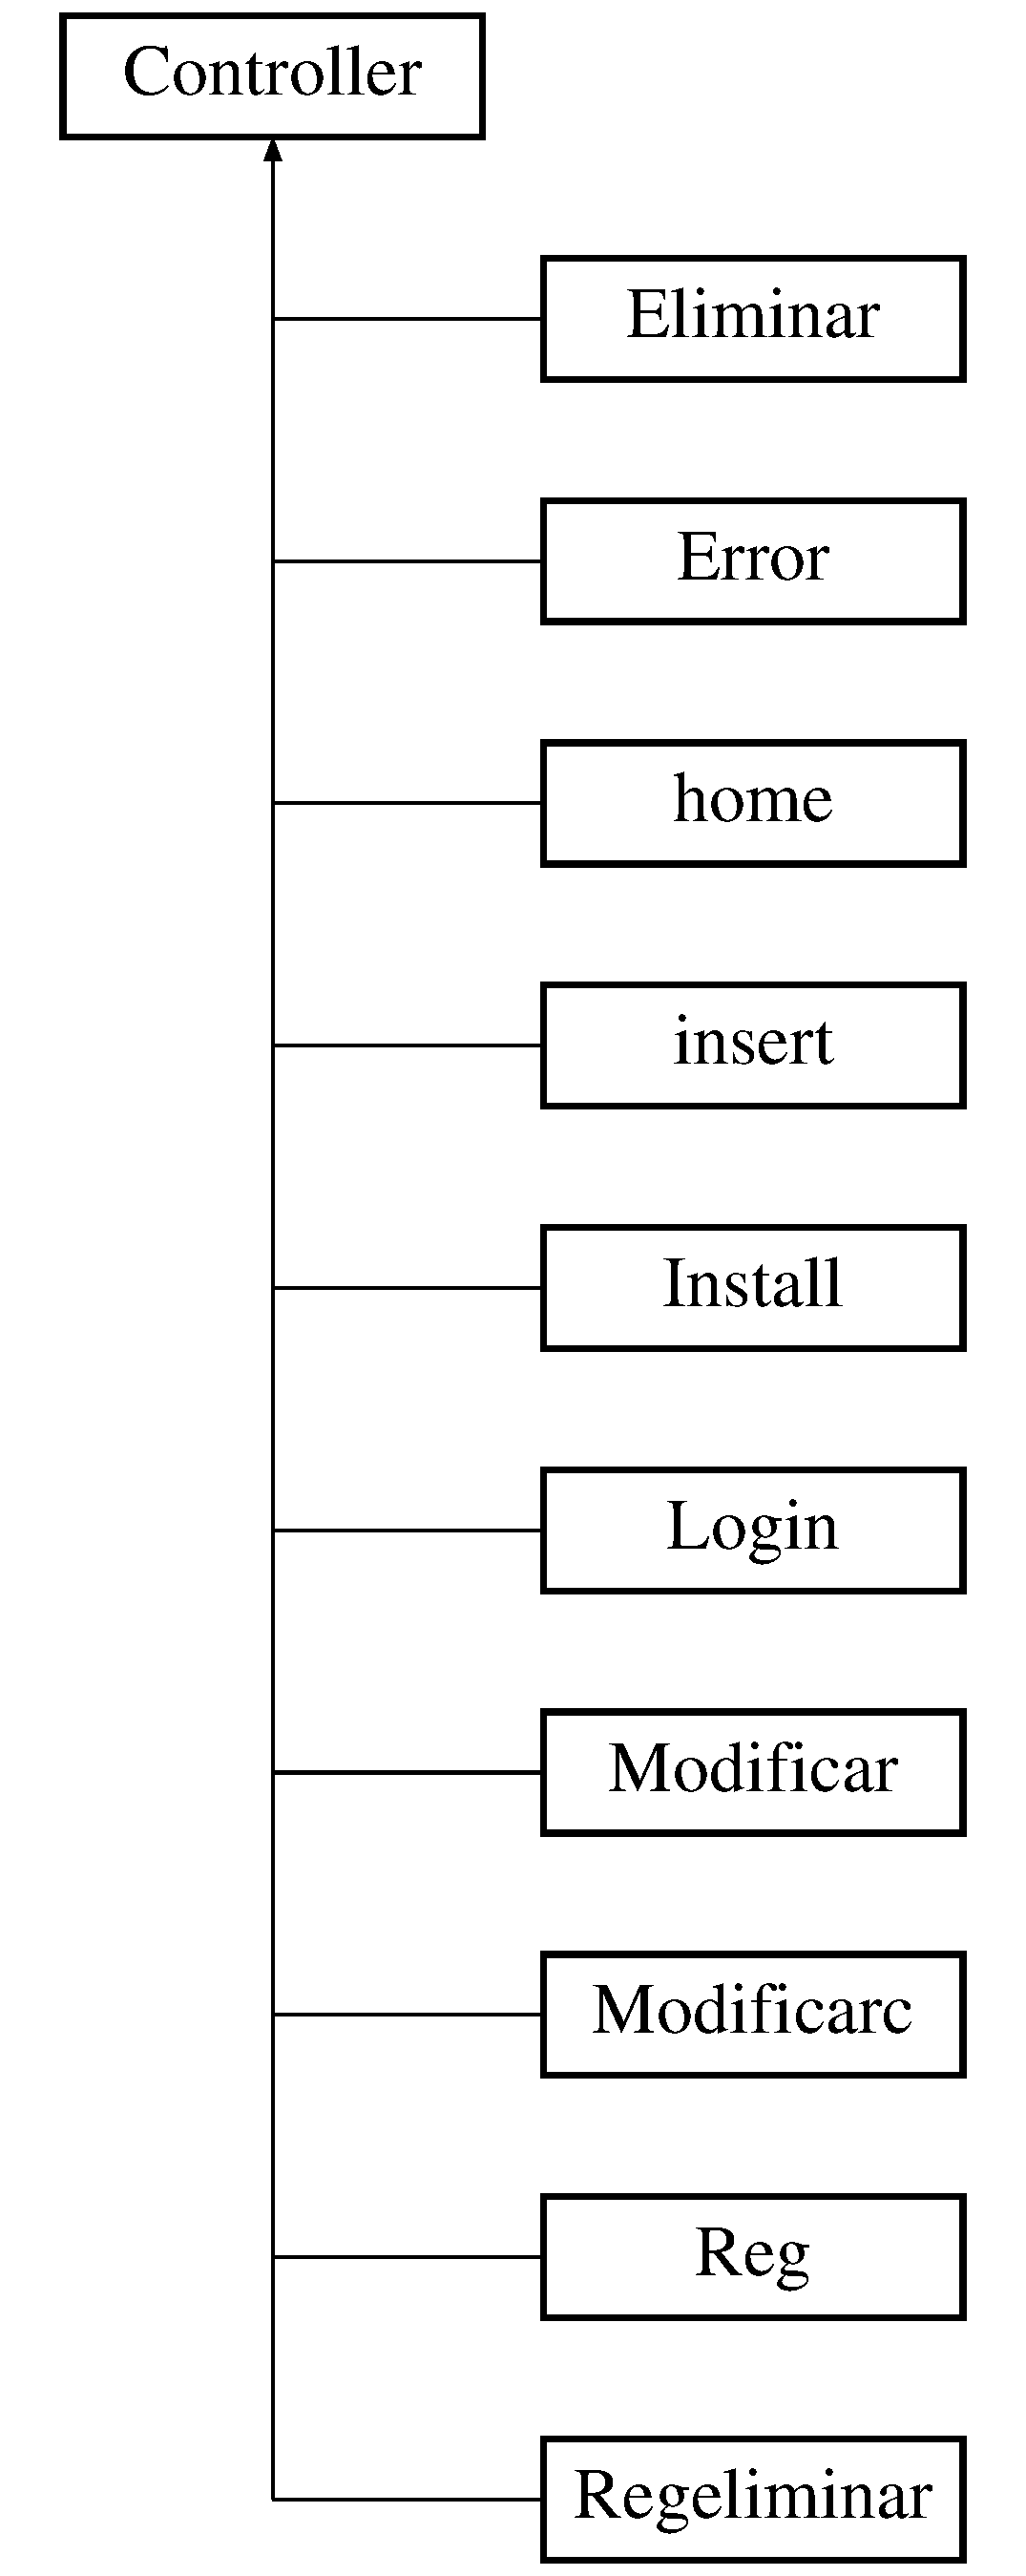
\includegraphics[height=11.000000cm]{class_controller}
\end{center}
\end{figure}
\subsection*{Métodos públicos}
\begin{DoxyCompactItemize}
\item 
\hypertarget{class_controller_a9162320adff1a1a4afd7f2372f753a3e}{}{\bfseries \+\_\+\+\_\+construct} (\$params)\label{class_controller_a9162320adff1a1a4afd7f2372f753a3e}

\item 
\hypertarget{class_controller_a185653cac2d8a82b6eb5aff50834e49d}{}{\bfseries ajax\+\_\+set} (\$output)\label{class_controller_a185653cac2d8a82b6eb5aff50834e49d}

\end{DoxyCompactItemize}
\subsection*{Atributos protegidos}
\begin{DoxyCompactItemize}
\item 
\hypertarget{class_controller_a08fdd91bde255dbe3e2d15a22d9663e8}{}{\bfseries \$model}\label{class_controller_a08fdd91bde255dbe3e2d15a22d9663e8}

\item 
\hypertarget{class_controller_acccf2eac8663e0cebe8101e90fbab089}{}{\bfseries \$view}\label{class_controller_acccf2eac8663e0cebe8101e90fbab089}

\item 
\hypertarget{class_controller_afe68e6fbe7acfbffc0af0c84a1996466}{}{\bfseries \$params}\label{class_controller_afe68e6fbe7acfbffc0af0c84a1996466}

\item 
\hypertarget{class_controller_ae4901046cc3e1deebf77ccc785384a78}{}{\bfseries \$conf}\label{class_controller_ae4901046cc3e1deebf77ccc785384a78}

\end{DoxyCompactItemize}


La documentación para esta clase fue generada a partir del siguiente fichero\+:\begin{DoxyCompactItemize}
\item 
sys/controller.\+php\end{DoxyCompactItemize}

\hypertarget{class_core}{}\section{Referencia de la Clase Core}
\label{class_core}\index{Core@{Core}}
\subsection*{Métodos públicos estáticos}
\begin{DoxyCompactItemize}
\item 
\hypertarget{class_core_a9f0be6ae273d3669e11c29910a0be338}{}static {\bfseries init} ()\label{class_core_a9f0be6ae273d3669e11c29910a0be338}

\item 
\hypertarget{class_core_a172c2b8bbed5f8e23ea32e08b665b59b}{}static {\bfseries router} ()\label{class_core_a172c2b8bbed5f8e23ea32e08b665b59b}

\end{DoxyCompactItemize}


La documentación para esta clase fue generada a partir del siguiente fichero\+:\begin{DoxyCompactItemize}
\item 
sys/core.\+php\end{DoxyCompactItemize}

\hypertarget{class_d_b}{}\section{Referencia de la Clase D\+B}
\label{class_d_b}\index{D\+B@{D\+B}}
Diagrama de herencias de D\+B\begin{figure}[H]
\begin{center}
\leavevmode
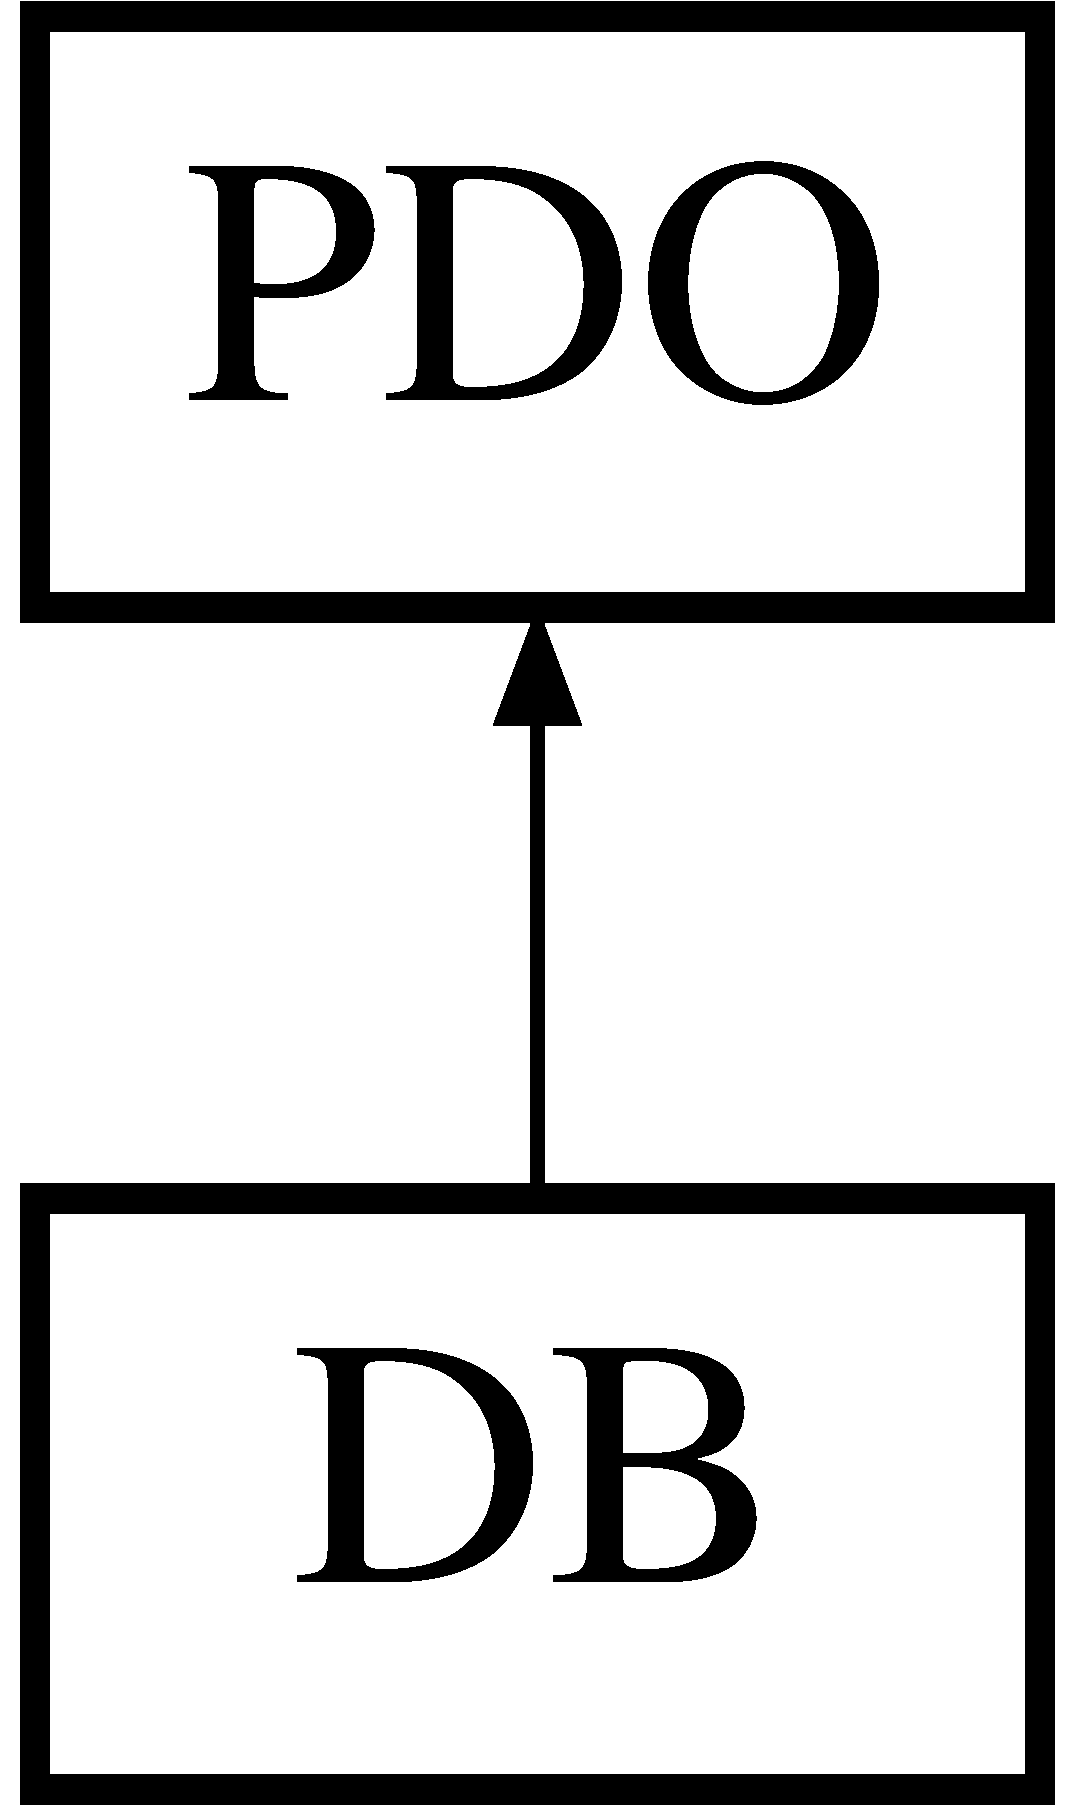
\includegraphics[height=2.000000cm]{class_d_b}
\end{center}
\end{figure}
\subsection*{Métodos públicos estáticos}
\begin{DoxyCompactItemize}
\item 
\hypertarget{class_d_b_af527068985bac6010736b5959643eda7}{}static {\bfseries singleton} ()\label{class_d_b_af527068985bac6010736b5959643eda7}

\end{DoxyCompactItemize}
\subsection*{Atributos públicos estáticos}
\begin{DoxyCompactItemize}
\item 
\hypertarget{class_d_b_ac350be23da328a6f5429313efc9b96e4}{}static {\bfseries \$\+\_\+instance}\label{class_d_b_ac350be23da328a6f5429313efc9b96e4}

\end{DoxyCompactItemize}


La documentación para esta clase fue generada a partir del siguiente fichero\+:\begin{DoxyCompactItemize}
\item 
sys/db.\+php\end{DoxyCompactItemize}

\hypertarget{class_eliminar}{}\section{Referencia de la Clase Eliminar}
\label{class_eliminar}\index{Eliminar@{Eliminar}}
Diagrama de herencias de Eliminar\begin{figure}[H]
\begin{center}
\leavevmode
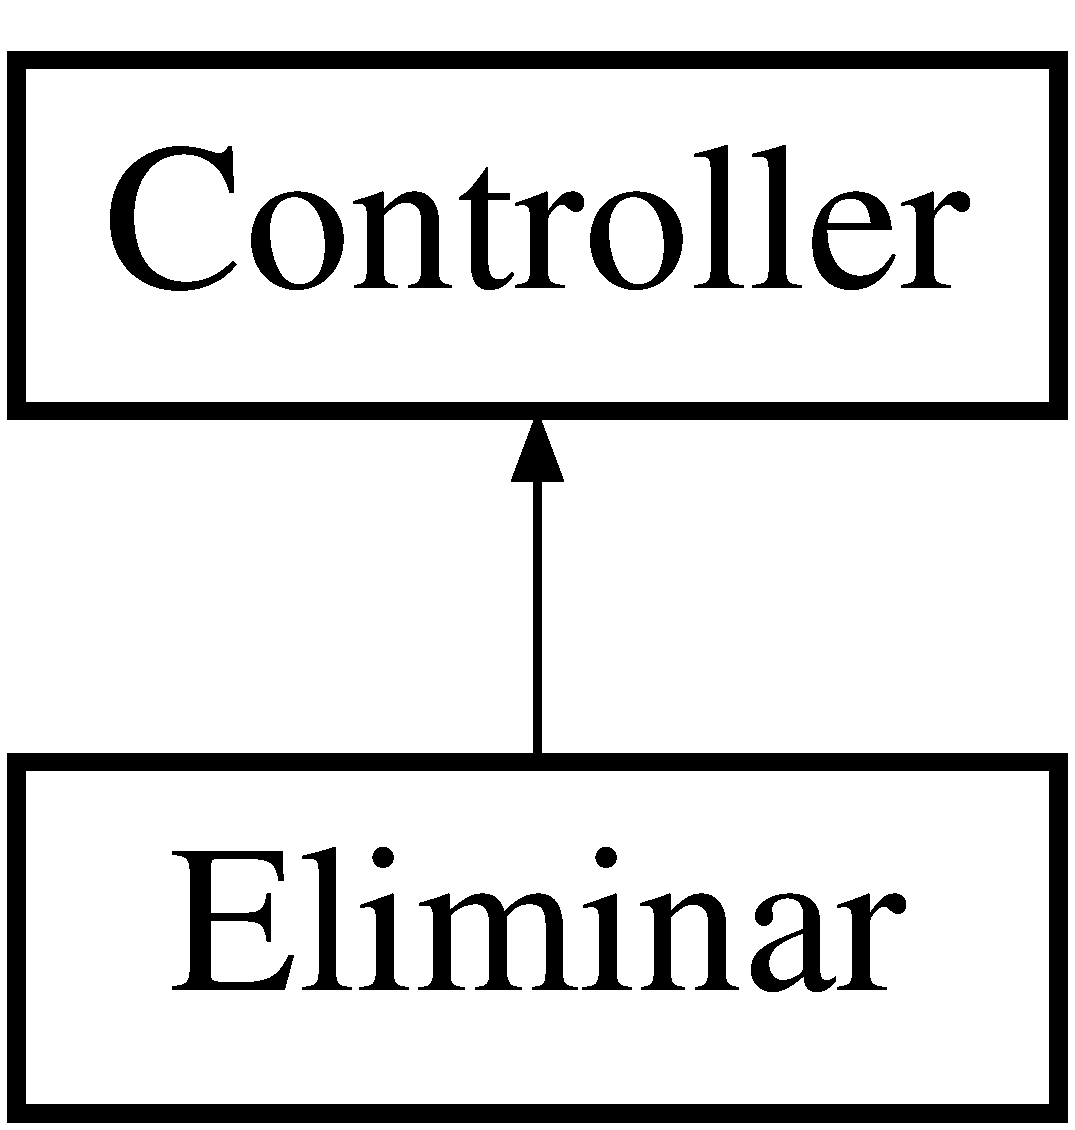
\includegraphics[height=2.000000cm]{class_eliminar}
\end{center}
\end{figure}
\subsection*{Métodos públicos}
\begin{DoxyCompactItemize}
\item 
\hypertarget{class_eliminar_a174b8e4c7d4d7363c6f773671defdeff}{}{\bfseries home} ()\label{class_eliminar_a174b8e4c7d4d7363c6f773671defdeff}

\item 
\hypertarget{class_eliminar_ae05738af445a2eb4f3456604f1b9be8f}{}{\bfseries eliminar} ()\label{class_eliminar_ae05738af445a2eb4f3456604f1b9be8f}

\end{DoxyCompactItemize}
\subsection*{Otros miembros heredados}


La documentación para esta clase fue generada a partir del siguiente fichero\+:\begin{DoxyCompactItemize}
\item 
app/controllers/eliminar.\+php\end{DoxyCompactItemize}

\hypertarget{class_error}{}\section{Referencia de la Clase Error}
\label{class_error}\index{Error@{Error}}
Diagrama de herencias de Error\begin{figure}[H]
\begin{center}
\leavevmode
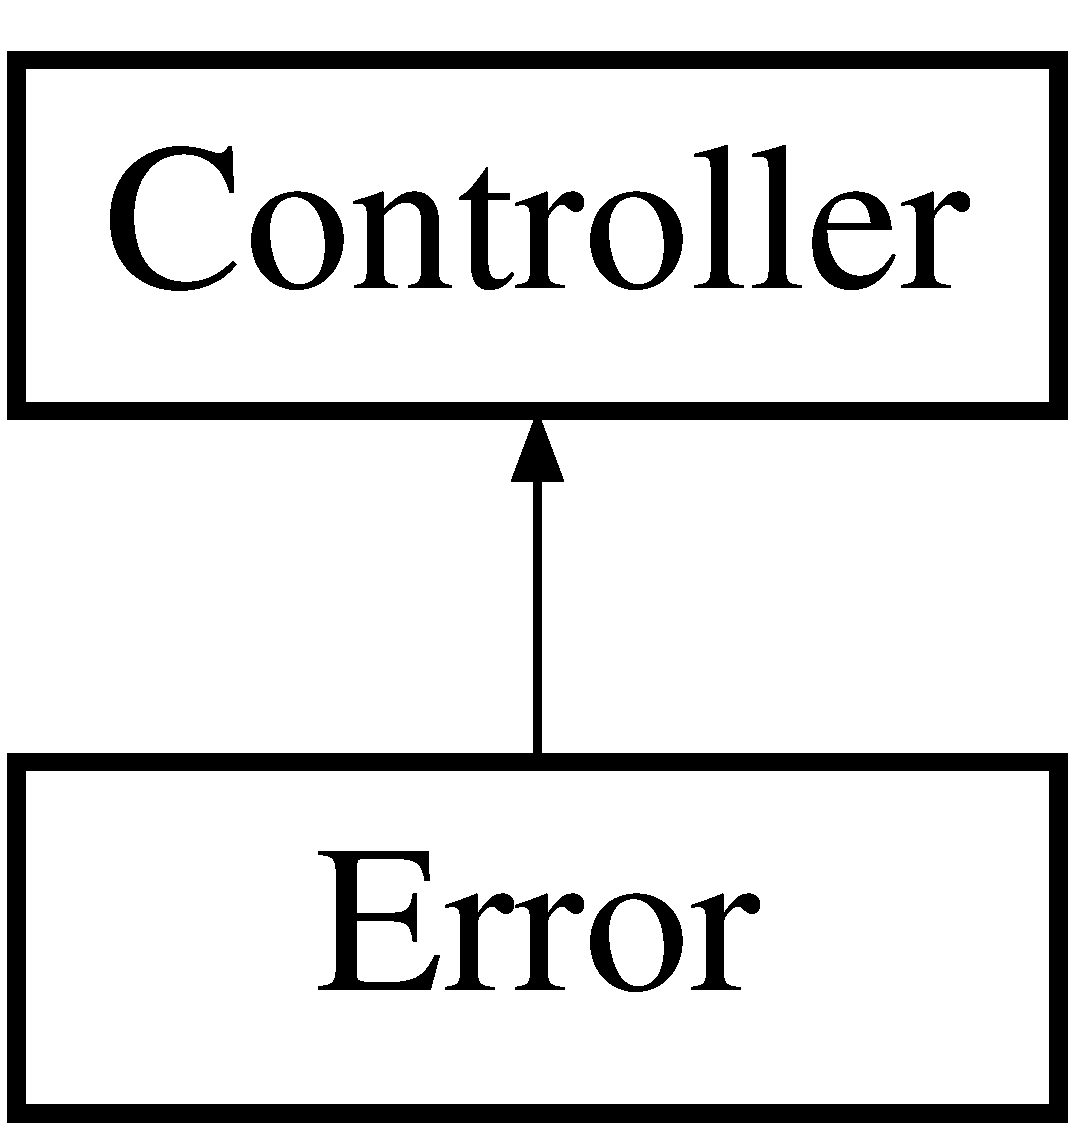
\includegraphics[height=2.000000cm]{class_error}
\end{center}
\end{figure}
\subsection*{Métodos públicos}
\begin{DoxyCompactItemize}
\item 
\hypertarget{class_error_a05014738840640fff5d40cc0604cb5c9}{}{\bfseries \+\_\+\+\_\+construct} (\$params=null)\label{class_error_a05014738840640fff5d40cc0604cb5c9}

\item 
\hypertarget{class_error_a174b8e4c7d4d7363c6f773671defdeff}{}{\bfseries home} ()\label{class_error_a174b8e4c7d4d7363c6f773671defdeff}

\end{DoxyCompactItemize}
\subsection*{Otros miembros heredados}


La documentación para esta clase fue generada a partir del siguiente fichero\+:\begin{DoxyCompactItemize}
\item 
app/controllers/error.\+php\end{DoxyCompactItemize}

\hypertarget{classhome}{}\section{Referencia de la Clase home}
\label{classhome}\index{home@{home}}
Diagrama de herencias de home\begin{figure}[H]
\begin{center}
\leavevmode
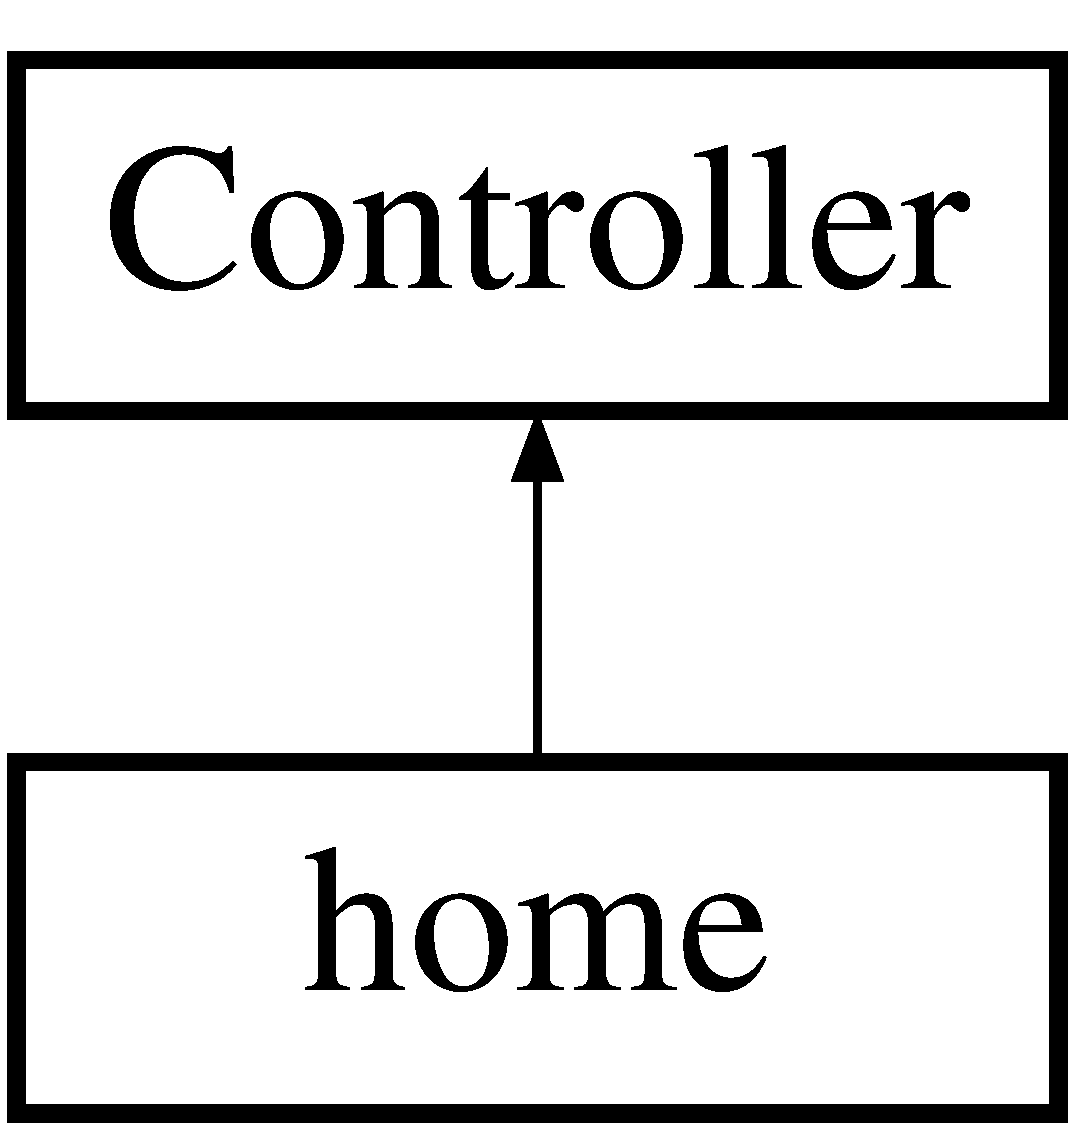
\includegraphics[height=2.000000cm]{classhome}
\end{center}
\end{figure}
\subsection*{Métodos públicos}
\begin{DoxyCompactItemize}
\item 
\hyperlink{classhome_a9162320adff1a1a4afd7f2372f753a3e}{\+\_\+\+\_\+construct} (\$params)
\item 
\hypertarget{classhome_a174b8e4c7d4d7363c6f773671defdeff}{}{\bfseries home} ()\label{classhome_a174b8e4c7d4d7363c6f773671defdeff}

\item 
\hyperlink{classhome_aa311da27ba5706f5710cea7706c8eae1}{login} ()
\item 
\hypertarget{classhome_ae640d82759dd7439b2d6611c41f6478b}{}{\bfseries salir} ()\label{classhome_ae640d82759dd7439b2d6611c41f6478b}

\end{DoxyCompactItemize}
\subsection*{Otros miembros heredados}


\subsection{Documentación del constructor y destructor}
\hypertarget{classhome_a9162320adff1a1a4afd7f2372f753a3e}{}\index{home@{home}!\+\_\+\+\_\+construct@{\+\_\+\+\_\+construct}}
\index{\+\_\+\+\_\+construct@{\+\_\+\+\_\+construct}!home@{home}}
\subsubsection[{\+\_\+\+\_\+construct}]{\setlength{\rightskip}{0pt plus 5cm}\+\_\+\+\_\+construct (
\begin{DoxyParamCaption}
\item[{}]{\$params}
\end{DoxyParamCaption}
)}\label{classhome_a9162320adff1a1a4afd7f2372f753a3e}
Constructor

\subsection{Documentación de las funciones miembro}
\hypertarget{classhome_aa311da27ba5706f5710cea7706c8eae1}{}\index{home@{home}!login@{login}}
\index{login@{login}!home@{home}}
\subsubsection[{login}]{\setlength{\rightskip}{0pt plus 5cm}login (
\begin{DoxyParamCaption}
{}
\end{DoxyParamCaption}
)}\label{classhome_aa311da27ba5706f5710cea7706c8eae1}
Hace el login


\begin{DoxyParams}{Parámetros}
{\em nada} & \\
\hline
\end{DoxyParams}
\begin{DoxyReturn}{Devuelve}
login/home
\end{DoxyReturn}


La documentación para esta clase fue generada a partir del siguiente fichero\+:\begin{DoxyCompactItemize}
\item 
app/controllers/home.\+php\end{DoxyCompactItemize}

\hypertarget{classinsert}{}\section{Referencia de la Clase insert}
\label{classinsert}\index{insert@{insert}}
Diagrama de herencias de insert\begin{figure}[H]
\begin{center}
\leavevmode
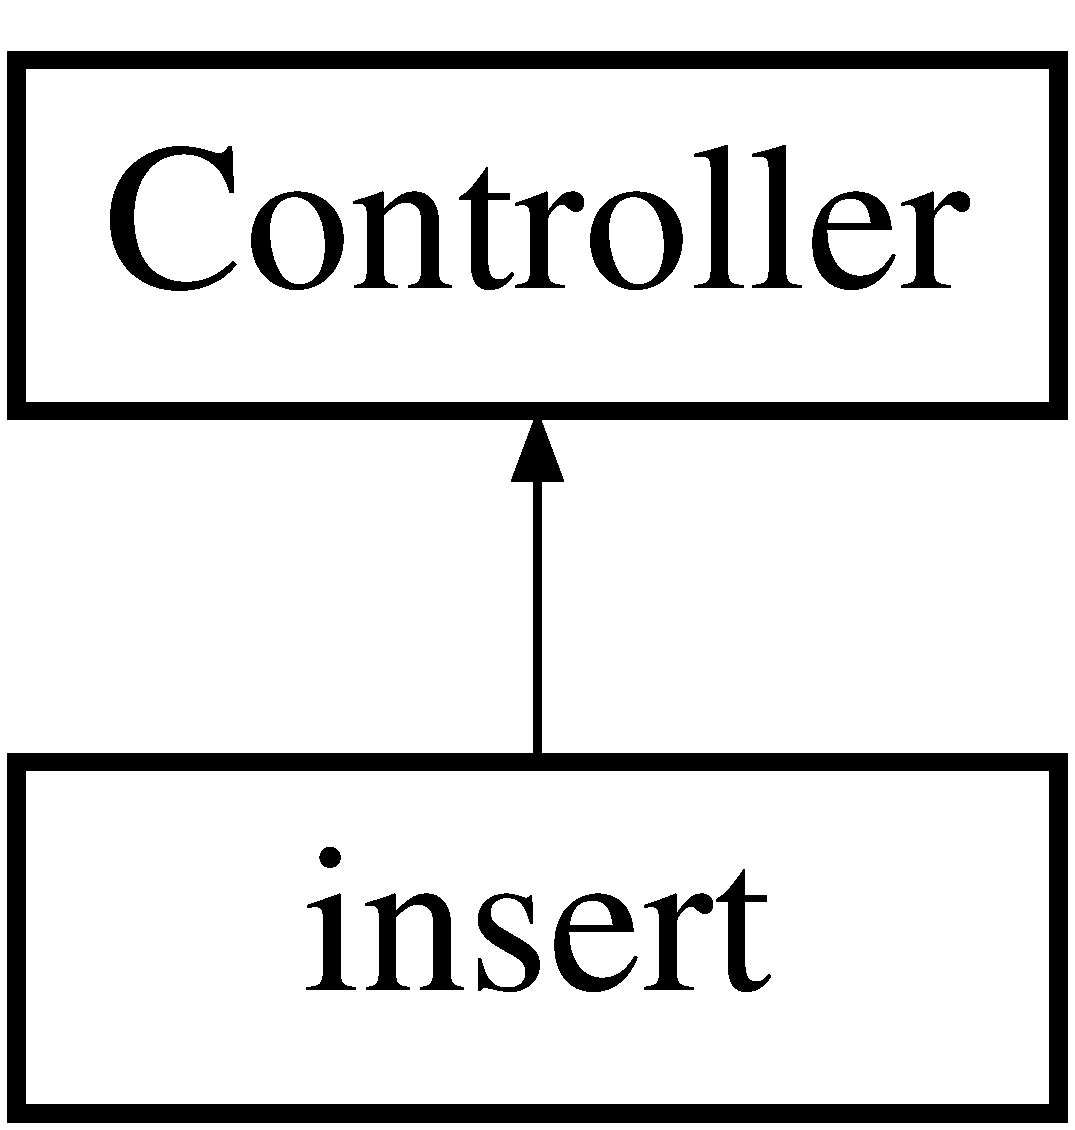
\includegraphics[height=2.000000cm]{classinsert}
\end{center}
\end{figure}
\subsection*{Métodos públicos}
\begin{DoxyCompactItemize}
\item 
\hypertarget{classinsert_a9162320adff1a1a4afd7f2372f753a3e}{}{\bfseries \+\_\+\+\_\+construct} (\$params)\label{classinsert_a9162320adff1a1a4afd7f2372f753a3e}

\item 
\hypertarget{classinsert_a174b8e4c7d4d7363c6f773671defdeff}{}{\bfseries home} ()\label{classinsert_a174b8e4c7d4d7363c6f773671defdeff}

\item 
\hypertarget{classinsert_a473241246338cfccc4709ba896749019}{}{\bfseries insert} ()\label{classinsert_a473241246338cfccc4709ba896749019}

\end{DoxyCompactItemize}
\subsection*{Otros miembros heredados}


La documentación para esta clase fue generada a partir del siguiente fichero\+:\begin{DoxyCompactItemize}
\item 
app/controllers/insert.\+php\end{DoxyCompactItemize}

\hypertarget{class_install}{}\section{Referencia de la Clase Install}
\label{class_install}\index{Install@{Install}}
Diagrama de herencias de Install\begin{figure}[H]
\begin{center}
\leavevmode
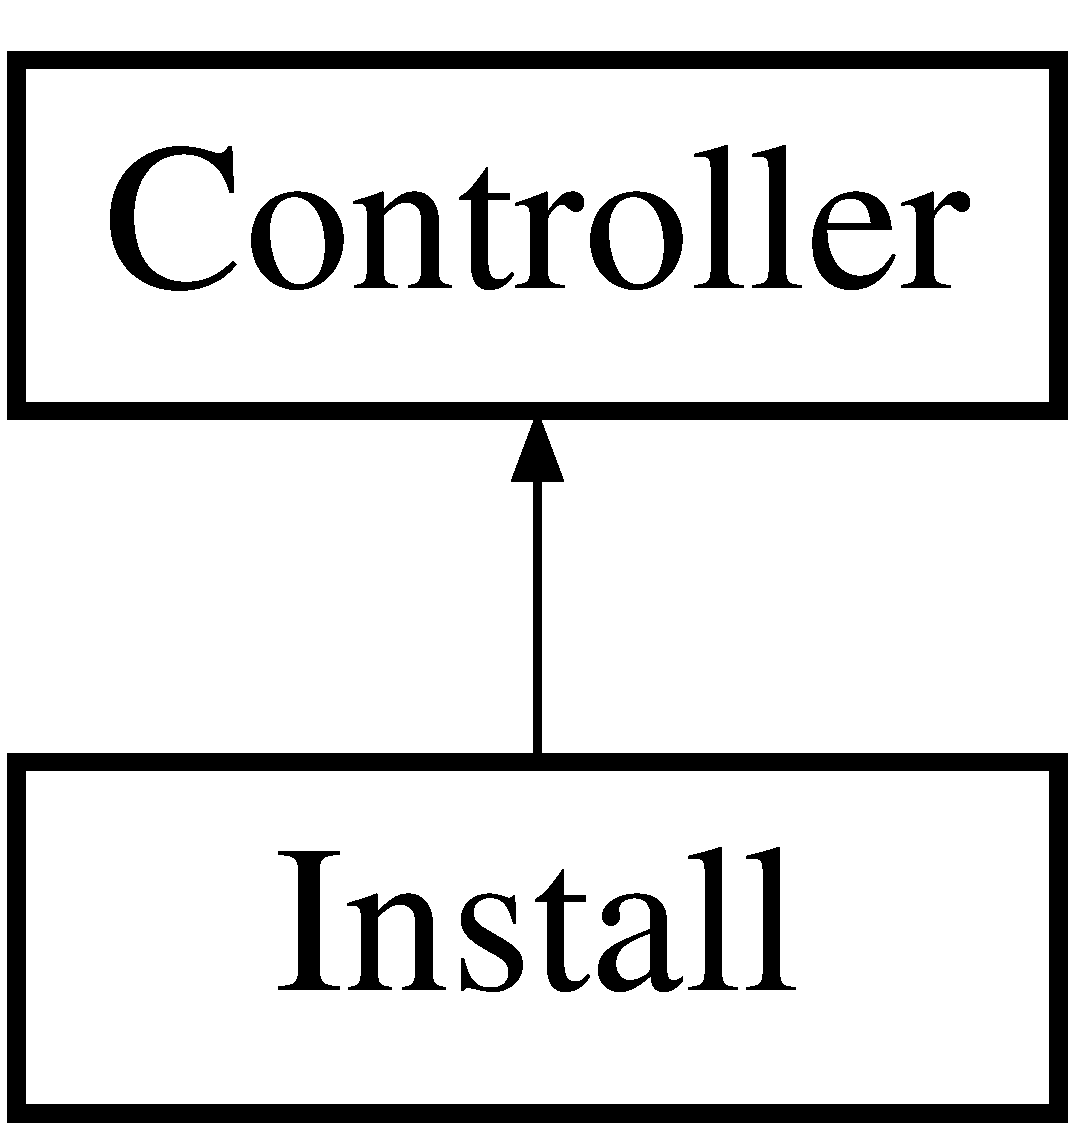
\includegraphics[height=2.000000cm]{class_install}
\end{center}
\end{figure}
\subsection*{Métodos públicos}
\begin{DoxyCompactItemize}
\item 
\hypertarget{class_install_a9162320adff1a1a4afd7f2372f753a3e}{}{\bfseries \+\_\+\+\_\+construct} (\$params)\label{class_install_a9162320adff1a1a4afd7f2372f753a3e}

\item 
\hypertarget{class_install_a174b8e4c7d4d7363c6f773671defdeff}{}{\bfseries home} ()\label{class_install_a174b8e4c7d4d7363c6f773671defdeff}

\item 
\hypertarget{class_install_a435e7d7525d4bcd0ed5e34a469f3adf6}{}{\bfseries create} ()\label{class_install_a435e7d7525d4bcd0ed5e34a469f3adf6}

\end{DoxyCompactItemize}
\subsection*{Otros miembros heredados}


La documentación para esta clase fue generada a partir del siguiente fichero\+:\begin{DoxyCompactItemize}
\item 
app/controllers/install.\+php\end{DoxyCompactItemize}

\hypertarget{class_k_autoloader}{}\section{Referencia de la Clase K\+Autoloader}
\label{class_k_autoloader}\index{K\+Autoloader@{K\+Autoloader}}
\subsection*{Métodos públicos estáticos}
\begin{DoxyCompactItemize}
\item 
\hypertarget{class_k_autoloader_a9c03232b28f4306eb55e5ae48d9b5a57}{}static {\bfseries Sys\+Loader} (\$class)\label{class_k_autoloader_a9c03232b28f4306eb55e5ae48d9b5a57}

\item 
\hypertarget{class_k_autoloader_ae9c99c78ae285712998aab4fcc0777bc}{}static {\bfseries App\+Cont\+Loader} (\$class)\label{class_k_autoloader_ae9c99c78ae285712998aab4fcc0777bc}

\item 
\hypertarget{class_k_autoloader_aa1675c8b9b03dc3c377ddfdbfef11b84}{}static {\bfseries App\+Mod\+Loader} (\$class)\label{class_k_autoloader_aa1675c8b9b03dc3c377ddfdbfef11b84}

\item 
\hypertarget{class_k_autoloader_a6a413fe01a5949ed9048dd7f50132488}{}static {\bfseries App\+Vie\+Loader} (\$class)\label{class_k_autoloader_a6a413fe01a5949ed9048dd7f50132488}

\end{DoxyCompactItemize}


La documentación para esta clase fue generada a partir del siguiente fichero\+:\begin{DoxyCompactItemize}
\item 
sys/helper.\+php\end{DoxyCompactItemize}

\hypertarget{class_login}{}\section{Referencia de la Clase Login}
\label{class_login}\index{Login@{Login}}
Diagrama de herencias de Login\begin{figure}[H]
\begin{center}
\leavevmode
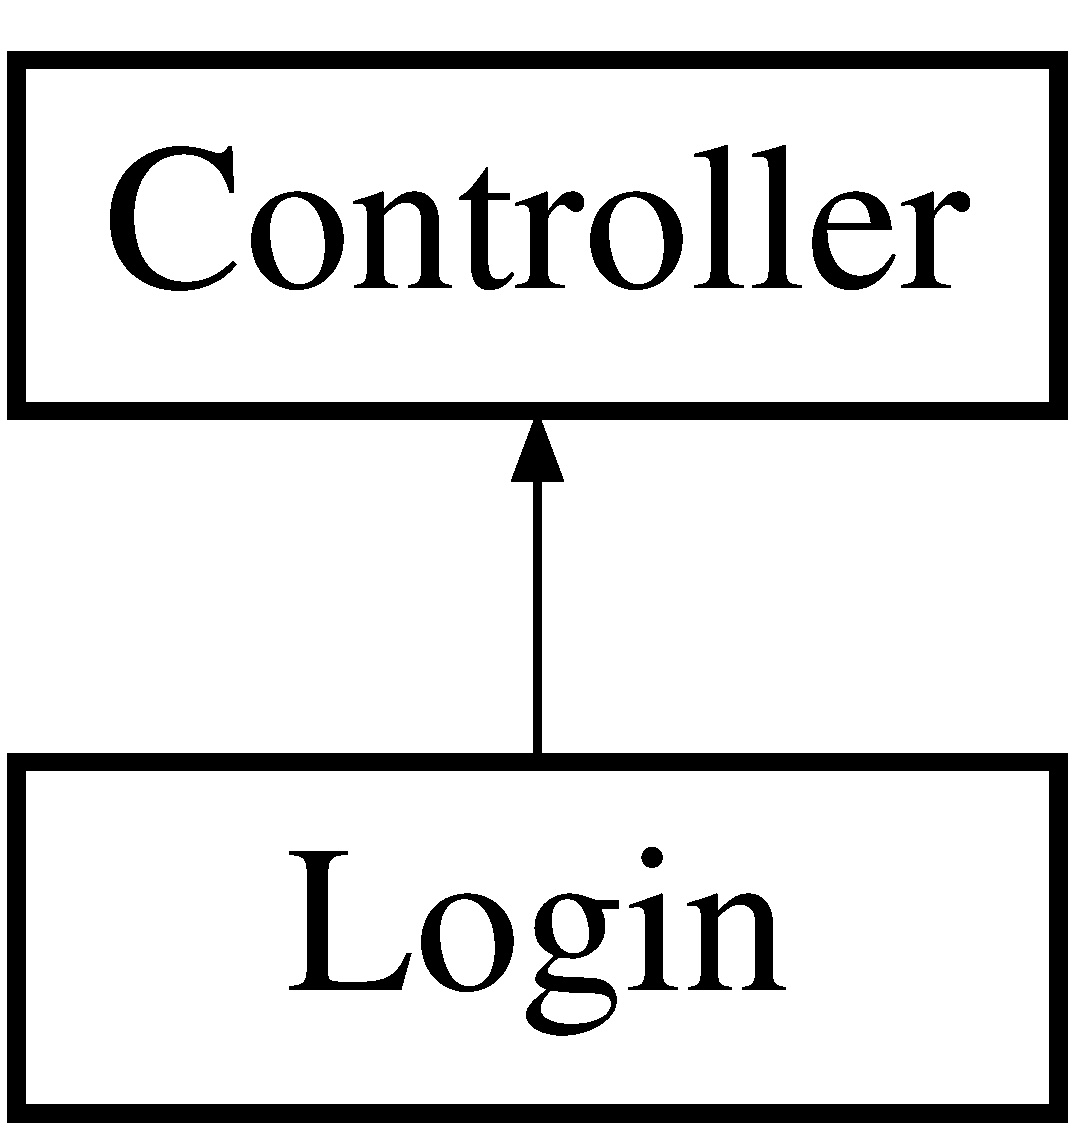
\includegraphics[height=2.000000cm]{class_login}
\end{center}
\end{figure}
\subsection*{Métodos públicos}
\begin{DoxyCompactItemize}
\item 
\hypertarget{class_login_a174b8e4c7d4d7363c6f773671defdeff}{}{\bfseries home} ()\label{class_login_a174b8e4c7d4d7363c6f773671defdeff}

\end{DoxyCompactItemize}
\subsection*{Otros miembros heredados}


La documentación para esta clase fue generada a partir del siguiente fichero\+:\begin{DoxyCompactItemize}
\item 
app/controllers/login.\+php\end{DoxyCompactItemize}

\hypertarget{classm_eliminar}{}\section{Referencia de la Clase m\+Eliminar}
\label{classm_eliminar}\index{m\+Eliminar@{m\+Eliminar}}
Diagrama de herencias de m\+Eliminar\begin{figure}[H]
\begin{center}
\leavevmode
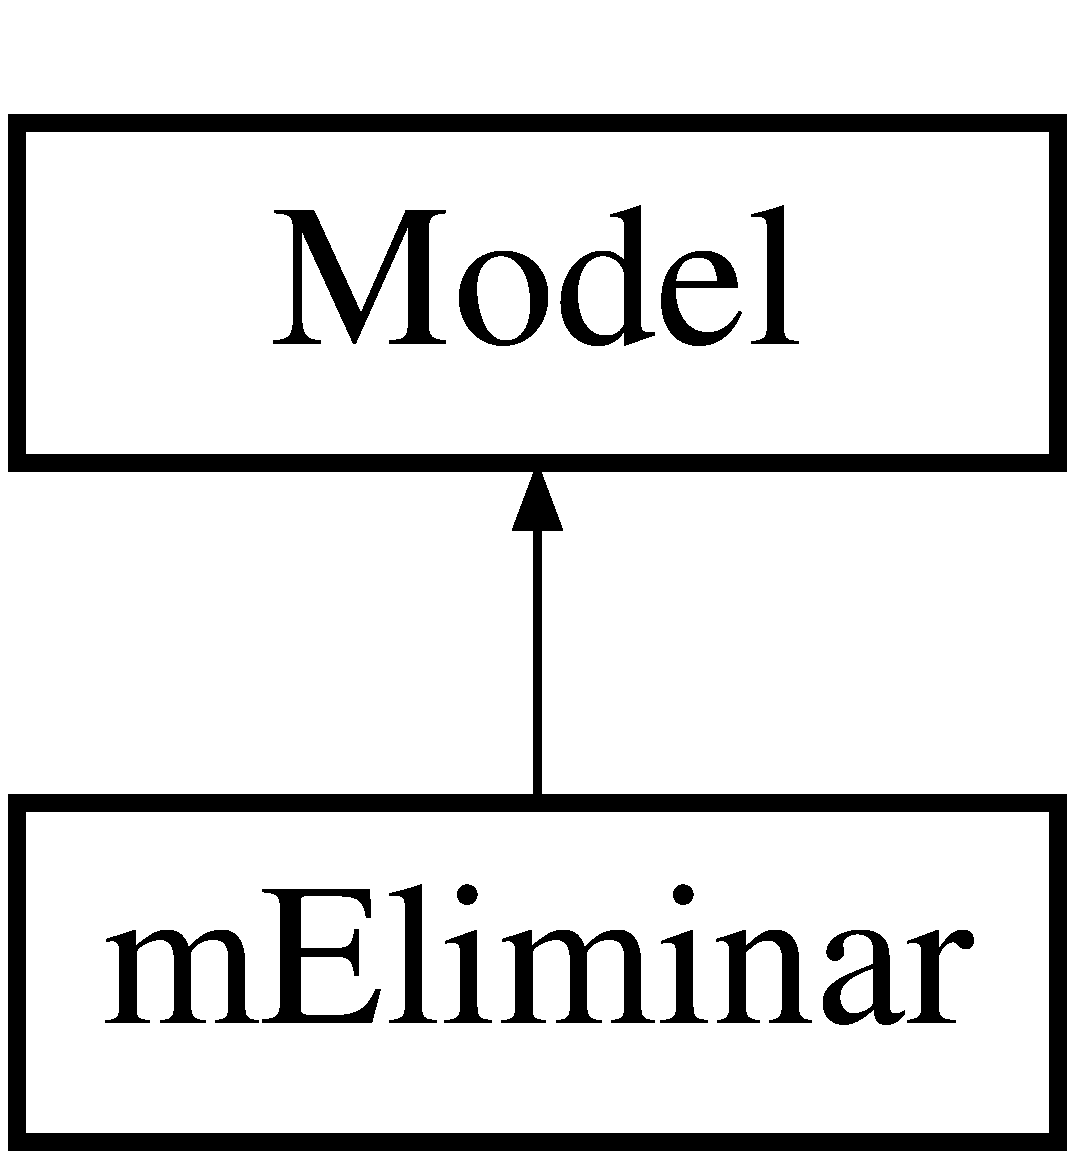
\includegraphics[height=2.000000cm]{classm_eliminar}
\end{center}
\end{figure}
\subsection*{Métodos públicos}
\begin{DoxyCompactItemize}
\item 
\hypertarget{classm_eliminar_ab934c86dd926a71481946464ce83c580}{}{\bfseries eliminar} (\$nusuario, \$password)\label{classm_eliminar_ab934c86dd926a71481946464ce83c580}

\end{DoxyCompactItemize}
\subsection*{Otros miembros heredados}


La documentación para esta clase fue generada a partir del siguiente fichero\+:\begin{DoxyCompactItemize}
\item 
app/models/meliminar.\+php\end{DoxyCompactItemize}

\hypertarget{classm_error}{}\section{Referencia de la Clase m\+Error}
\label{classm_error}\index{m\+Error@{m\+Error}}
Diagrama de herencias de m\+Error\begin{figure}[H]
\begin{center}
\leavevmode
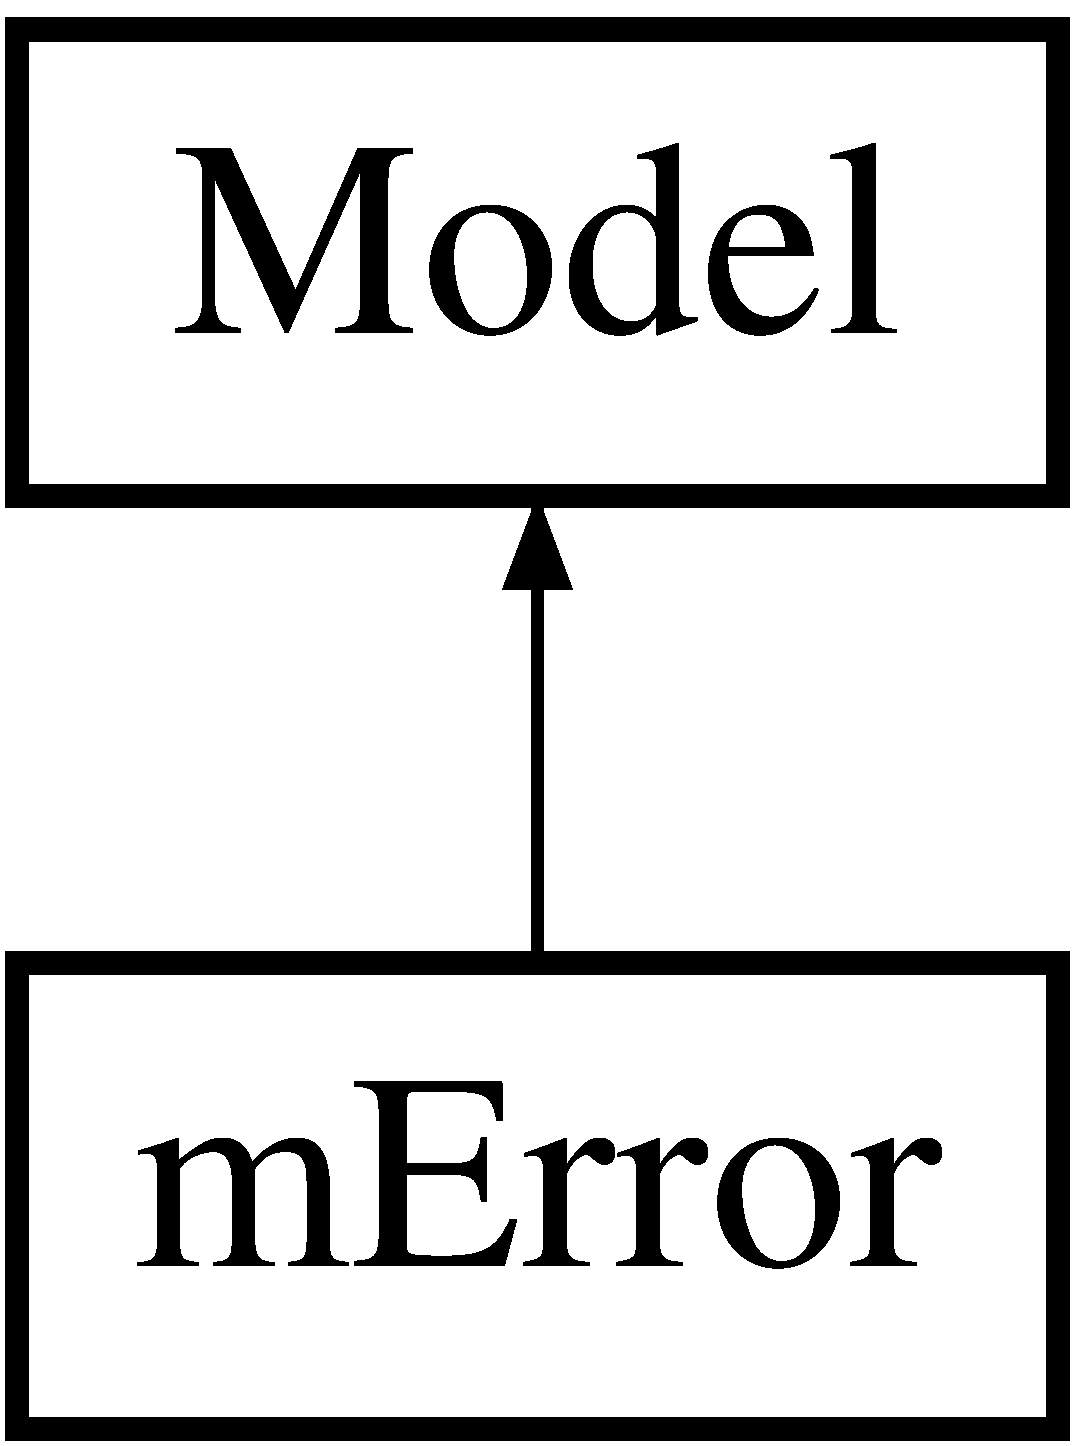
\includegraphics[height=2.000000cm]{classm_error}
\end{center}
\end{figure}
\subsection*{Otros miembros heredados}


La documentación para esta clase fue generada a partir del siguiente fichero\+:\begin{DoxyCompactItemize}
\item 
app/models/merror.\+php\end{DoxyCompactItemize}

\hypertarget{classm_home}{}\section{Referencia de la Clase m\+Home}
\label{classm_home}\index{m\+Home@{m\+Home}}
Diagrama de herencias de m\+Home\begin{figure}[H]
\begin{center}
\leavevmode
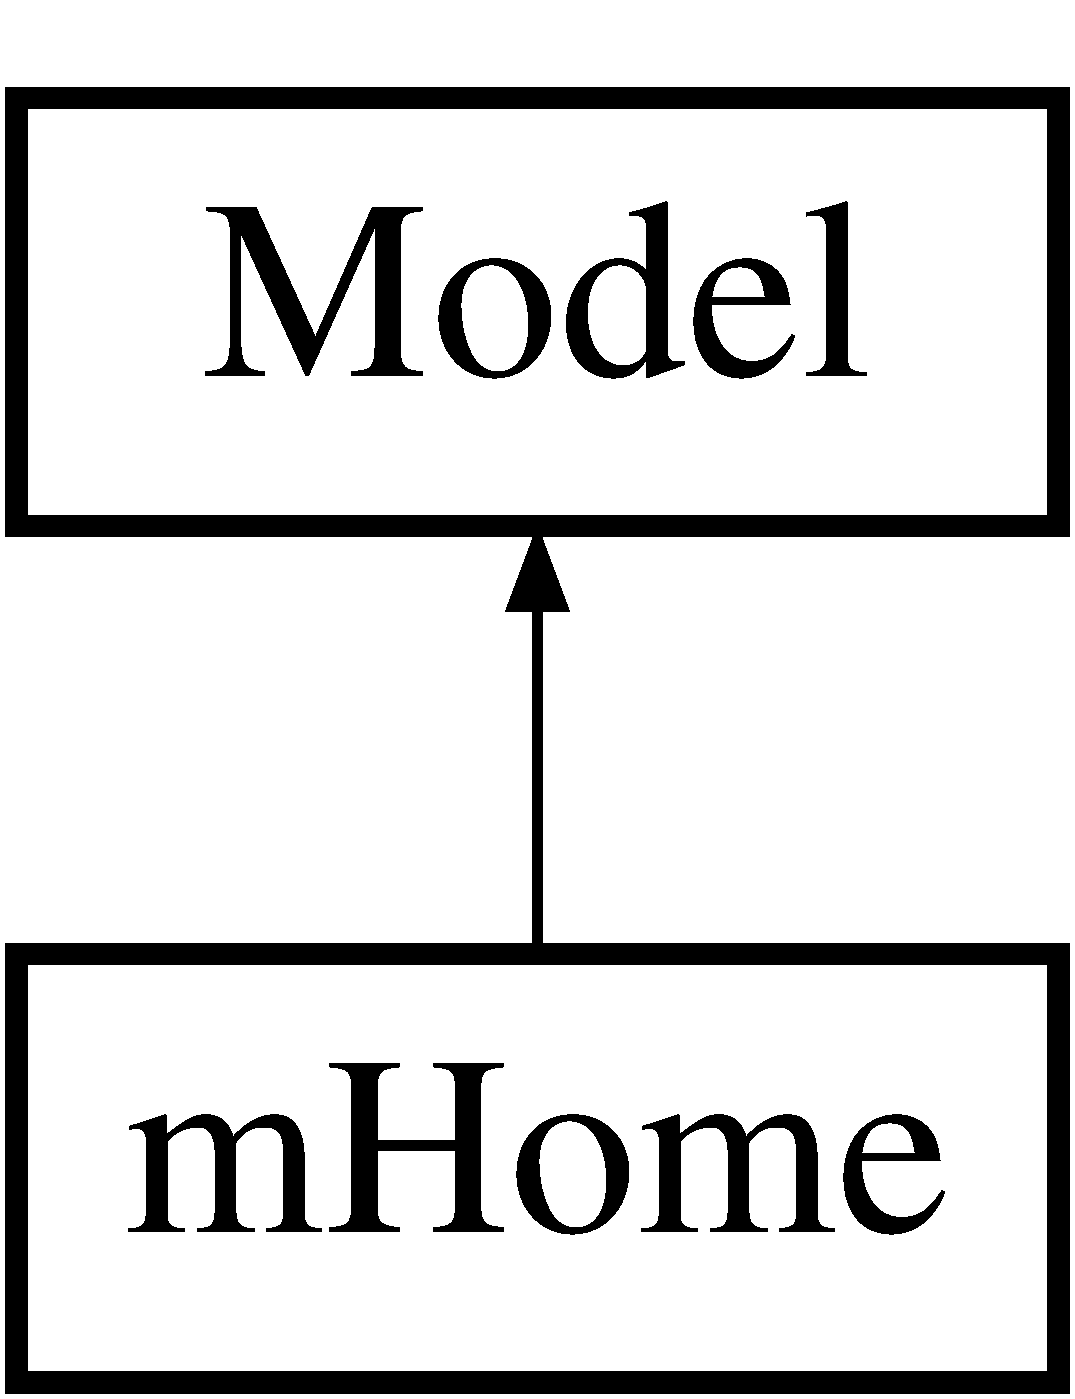
\includegraphics[height=2.000000cm]{classm_home}
\end{center}
\end{figure}
\subsection*{Métodos públicos}
\begin{DoxyCompactItemize}
\item 
\hypertarget{classm_home_a9162320adff1a1a4afd7f2372f753a3e}{}{\bfseries \+\_\+\+\_\+construct} (\$params)\label{classm_home_a9162320adff1a1a4afd7f2372f753a3e}

\item 
\hypertarget{classm_home_aa67567dc404200190a6abcae9262dba0}{}{\bfseries get\+\_\+out} ()\label{classm_home_aa67567dc404200190a6abcae9262dba0}

\item 
\hypertarget{classm_home_a3309f05cc3c0ac88c2ba466248d1d507}{}{\bfseries rol} (\$nusuario)\label{classm_home_a3309f05cc3c0ac88c2ba466248d1d507}

\item 
\hypertarget{classm_home_a1db2d12d379fffc4b5ae574167a1a799}{}{\bfseries login} (\$nusuario, \$password)\label{classm_home_a1db2d12d379fffc4b5ae574167a1a799}

\item 
\hypertarget{classm_home_a8fffd933aba0b9d7b1f927b2caca6966}{}{\bfseries insert} (\$idcliente, \$nusuario, \$password, \$rol)\label{classm_home_a8fffd933aba0b9d7b1f927b2caca6966}

\end{DoxyCompactItemize}
\subsection*{Otros miembros heredados}


La documentación para esta clase fue generada a partir del siguiente fichero\+:\begin{DoxyCompactItemize}
\item 
app/models/mhome.\+php\end{DoxyCompactItemize}

\hypertarget{classm_insert}{}\section{Referencia de la Clase m\+Insert}
\label{classm_insert}\index{m\+Insert@{m\+Insert}}
Diagrama de herencias de m\+Insert\begin{figure}[H]
\begin{center}
\leavevmode
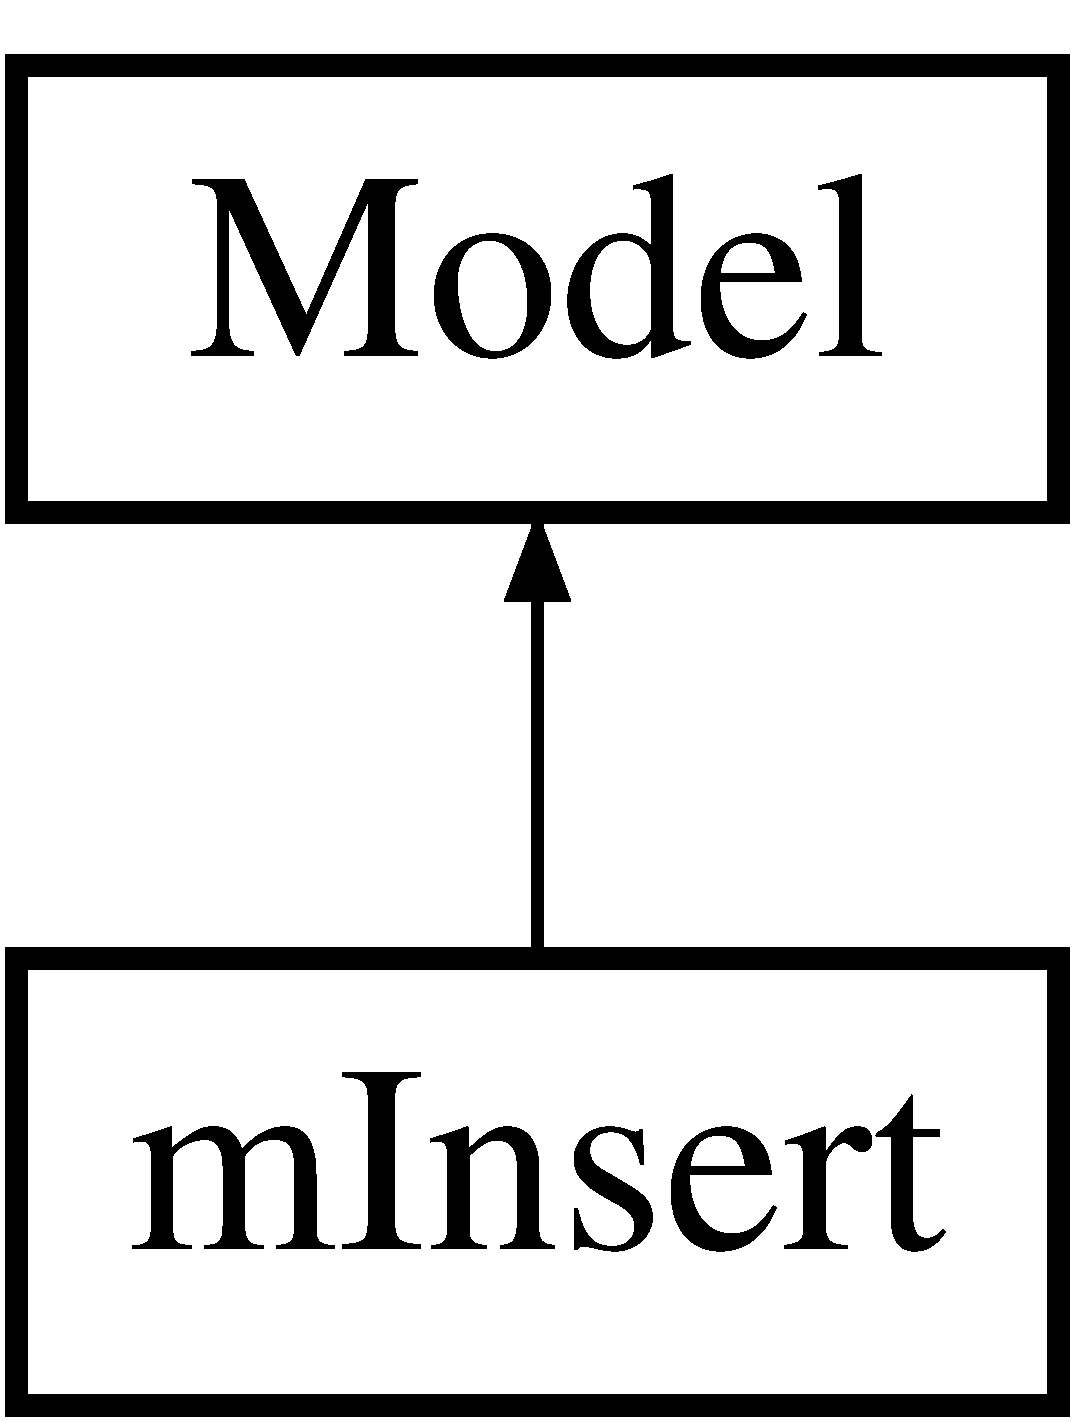
\includegraphics[height=2.000000cm]{classm_insert}
\end{center}
\end{figure}
\subsection*{Métodos públicos}
\begin{DoxyCompactItemize}
\item 
\hypertarget{classm_insert_a4294ecf2164cd0e0b13a7ec635f3cdd7}{}{\bfseries insert} (\$Nombre\+Compania, \$Nombre\+Contacto, \$D\+N\+I, \$Email, \$Cargo\+Contacto, \$Direccion, \$Ciudad, \$Region, \$Cod\+Postal, \$Pais, \$Telefono, \$Fax, \$Usuario, \$Password, \$Rol)\label{classm_insert_a4294ecf2164cd0e0b13a7ec635f3cdd7}

\end{DoxyCompactItemize}
\subsection*{Otros miembros heredados}


La documentación para esta clase fue generada a partir del siguiente fichero\+:\begin{DoxyCompactItemize}
\item 
app/models/minsert.\+php\end{DoxyCompactItemize}

\hypertarget{classm_install}{}\section{Referencia de la Clase m\+Install}
\label{classm_install}\index{m\+Install@{m\+Install}}
Diagrama de herencias de m\+Install\begin{figure}[H]
\begin{center}
\leavevmode
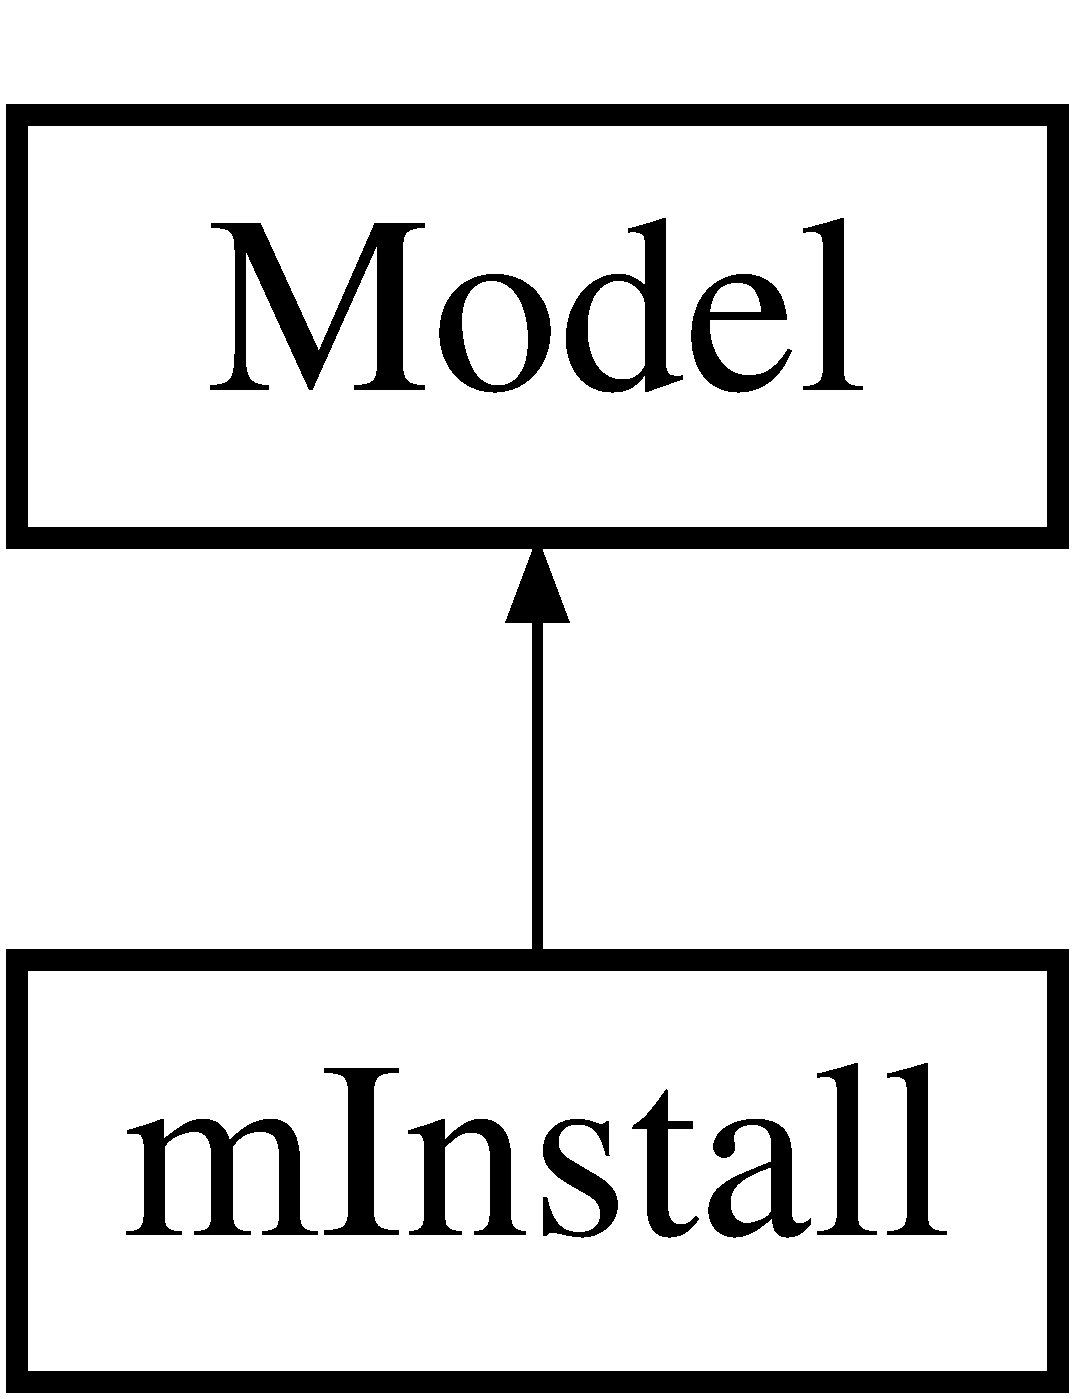
\includegraphics[height=2.000000cm]{classm_install}
\end{center}
\end{figure}
\subsection*{Métodos públicos}
\begin{DoxyCompactItemize}
\item 
\hypertarget{classm_install_a9162320adff1a1a4afd7f2372f753a3e}{}{\bfseries \+\_\+\+\_\+construct} (\$params)\label{classm_install_a9162320adff1a1a4afd7f2372f753a3e}

\item 
\hypertarget{classm_install_aa67567dc404200190a6abcae9262dba0}{}{\bfseries get\+\_\+out} ()\label{classm_install_aa67567dc404200190a6abcae9262dba0}

\item 
\hypertarget{classm_install_a730338378f77a6e490a10938166a6cc1}{}{\bfseries create} (\$dbname)\label{classm_install_a730338378f77a6e490a10938166a6cc1}

\item 
\hypertarget{classm_install_aa5e085eb04d3e6db625536f7e02a5d55}{}{\bfseries import} (\$mysql\+Host\+Name, \$mysql\+User\+Name, \$mysql\+Password, \$mysql\+Database\+Name, \$mysql\+Import\+Filename)\label{classm_install_aa5e085eb04d3e6db625536f7e02a5d55}

\end{DoxyCompactItemize}
\subsection*{Atributos protegidos}
\begin{DoxyCompactItemize}
\item 
\hypertarget{classm_install_ae4901046cc3e1deebf77ccc785384a78}{}{\bfseries \$conf}\label{classm_install_ae4901046cc3e1deebf77ccc785384a78}

\end{DoxyCompactItemize}


La documentación para esta clase fue generada a partir del siguiente fichero\+:\begin{DoxyCompactItemize}
\item 
app/models/minstall.\+php\end{DoxyCompactItemize}

\hypertarget{classm_login}{}\section{Referencia de la Clase m\+Login}
\label{classm_login}\index{m\+Login@{m\+Login}}
Diagrama de herencias de m\+Login\begin{figure}[H]
\begin{center}
\leavevmode
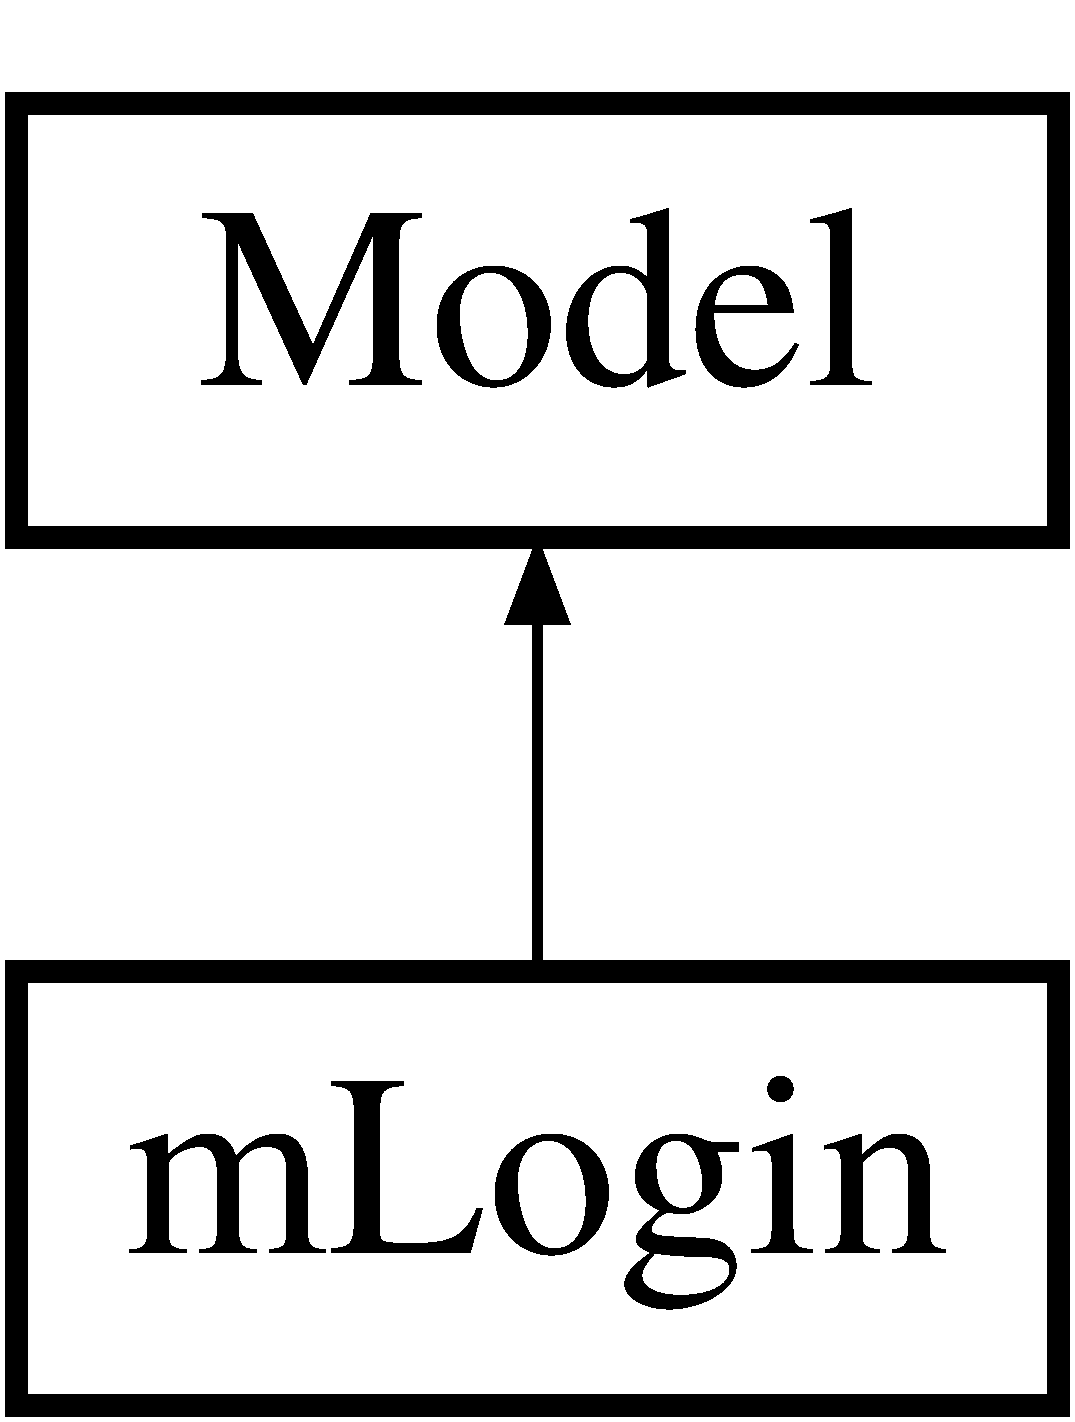
\includegraphics[height=2.000000cm]{classm_login}
\end{center}
\end{figure}
\subsection*{Otros miembros heredados}


La documentación para esta clase fue generada a partir del siguiente fichero\+:\begin{DoxyCompactItemize}
\item 
app/models/mlogin.\+php\end{DoxyCompactItemize}

\hypertarget{classm_modificar}{}\section{Referencia de la Clase m\+Modificar}
\label{classm_modificar}\index{m\+Modificar@{m\+Modificar}}
Diagrama de herencias de m\+Modificar\begin{figure}[H]
\begin{center}
\leavevmode
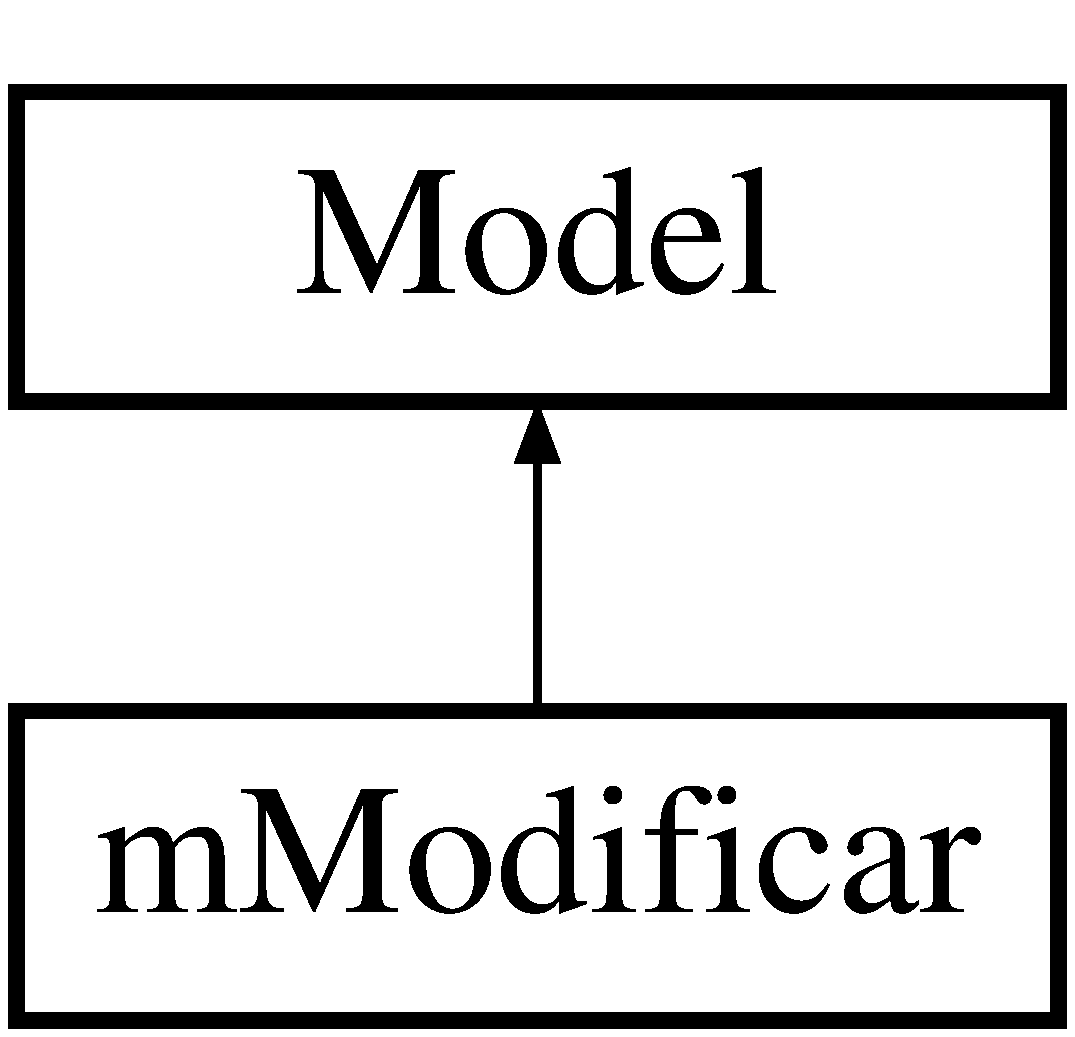
\includegraphics[height=2.000000cm]{classm_modificar}
\end{center}
\end{figure}
\subsection*{Métodos públicos}
\begin{DoxyCompactItemize}
\item 
\hypertarget{classm_modificar_a9162320adff1a1a4afd7f2372f753a3e}{}{\bfseries \+\_\+\+\_\+construct} (\$params)\label{classm_modificar_a9162320adff1a1a4afd7f2372f753a3e}

\item 
\hypertarget{classm_modificar_aa67567dc404200190a6abcae9262dba0}{}{\bfseries get\+\_\+out} ()\label{classm_modificar_aa67567dc404200190a6abcae9262dba0}

\item 
\hypertarget{classm_modificar_a3511064d552e515d53fbdf50fee29b6e}{}{\bfseries modificar} (\$Nombre\+Compania, \$Nombre\+Contacto, \$D\+N\+I, \$Email, \$Cargo\+Contacto, \$Direccion, \$Ciudad, \$Region, \$Cod\+Postal, \$Pais, \$Telefono, \$Fax, \$Usuario, \$Password, \$Rol)\label{classm_modificar_a3511064d552e515d53fbdf50fee29b6e}

\item 
\hypertarget{classm_modificar_a3f1df2d57246e91220a6a6e53c0f3e35}{}{\bfseries hola} ()\label{classm_modificar_a3f1df2d57246e91220a6a6e53c0f3e35}

\end{DoxyCompactItemize}
\subsection*{Otros miembros heredados}


La documentación para esta clase fue generada a partir del siguiente fichero\+:\begin{DoxyCompactItemize}
\item 
app/models/mmodificar.\+php\end{DoxyCompactItemize}

\hypertarget{classm_modificarc}{}\section{Referencia de la Clase m\+Modificarc}
\label{classm_modificarc}\index{m\+Modificarc@{m\+Modificarc}}
Diagrama de herencias de m\+Modificarc\begin{figure}[H]
\begin{center}
\leavevmode
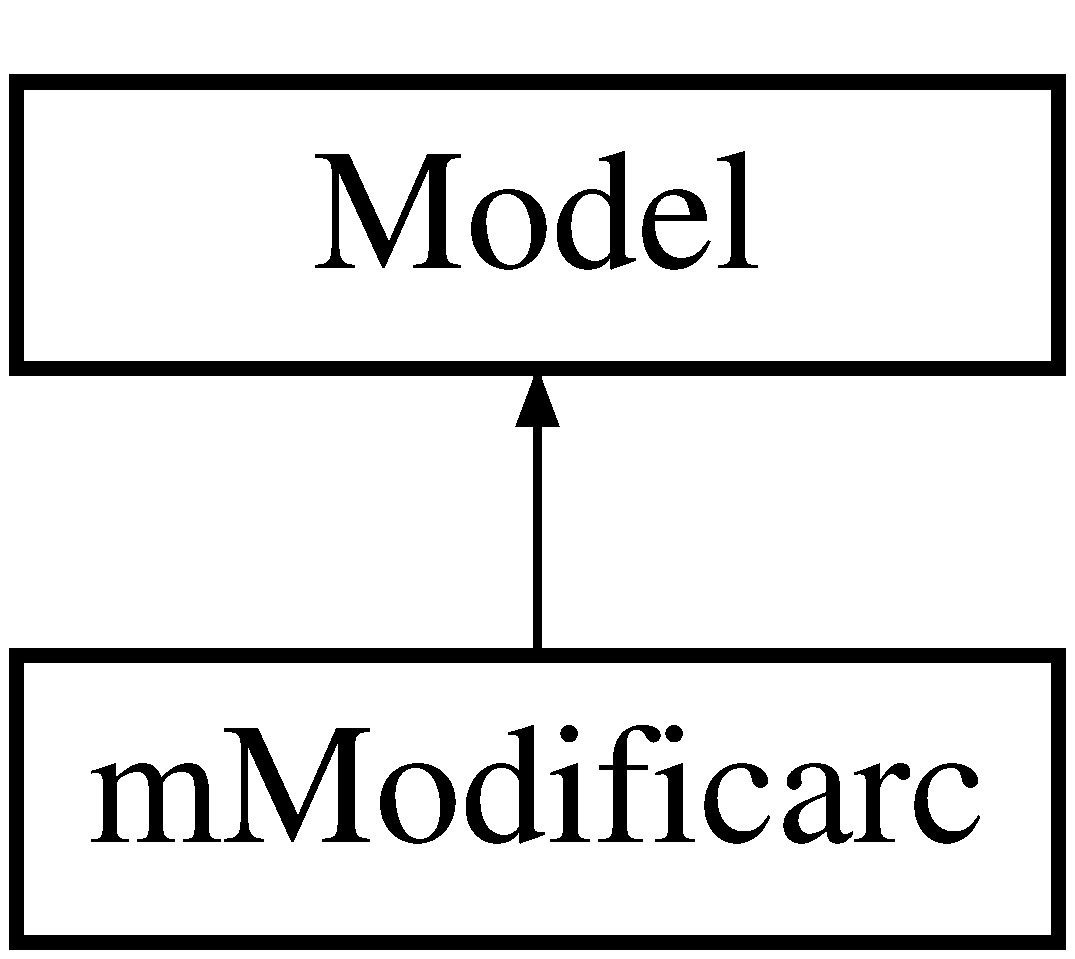
\includegraphics[height=2.000000cm]{classm_modificarc}
\end{center}
\end{figure}
\subsection*{Otros miembros heredados}


La documentación para esta clase fue generada a partir del siguiente fichero\+:\begin{DoxyCompactItemize}
\item 
app/models/mmodificarc.\+php\end{DoxyCompactItemize}

\hypertarget{class_model}{}\section{Referencia de la Clase Model}
\label{class_model}\index{Model@{Model}}
Diagrama de herencias de Model\begin{figure}[H]
\begin{center}
\leavevmode
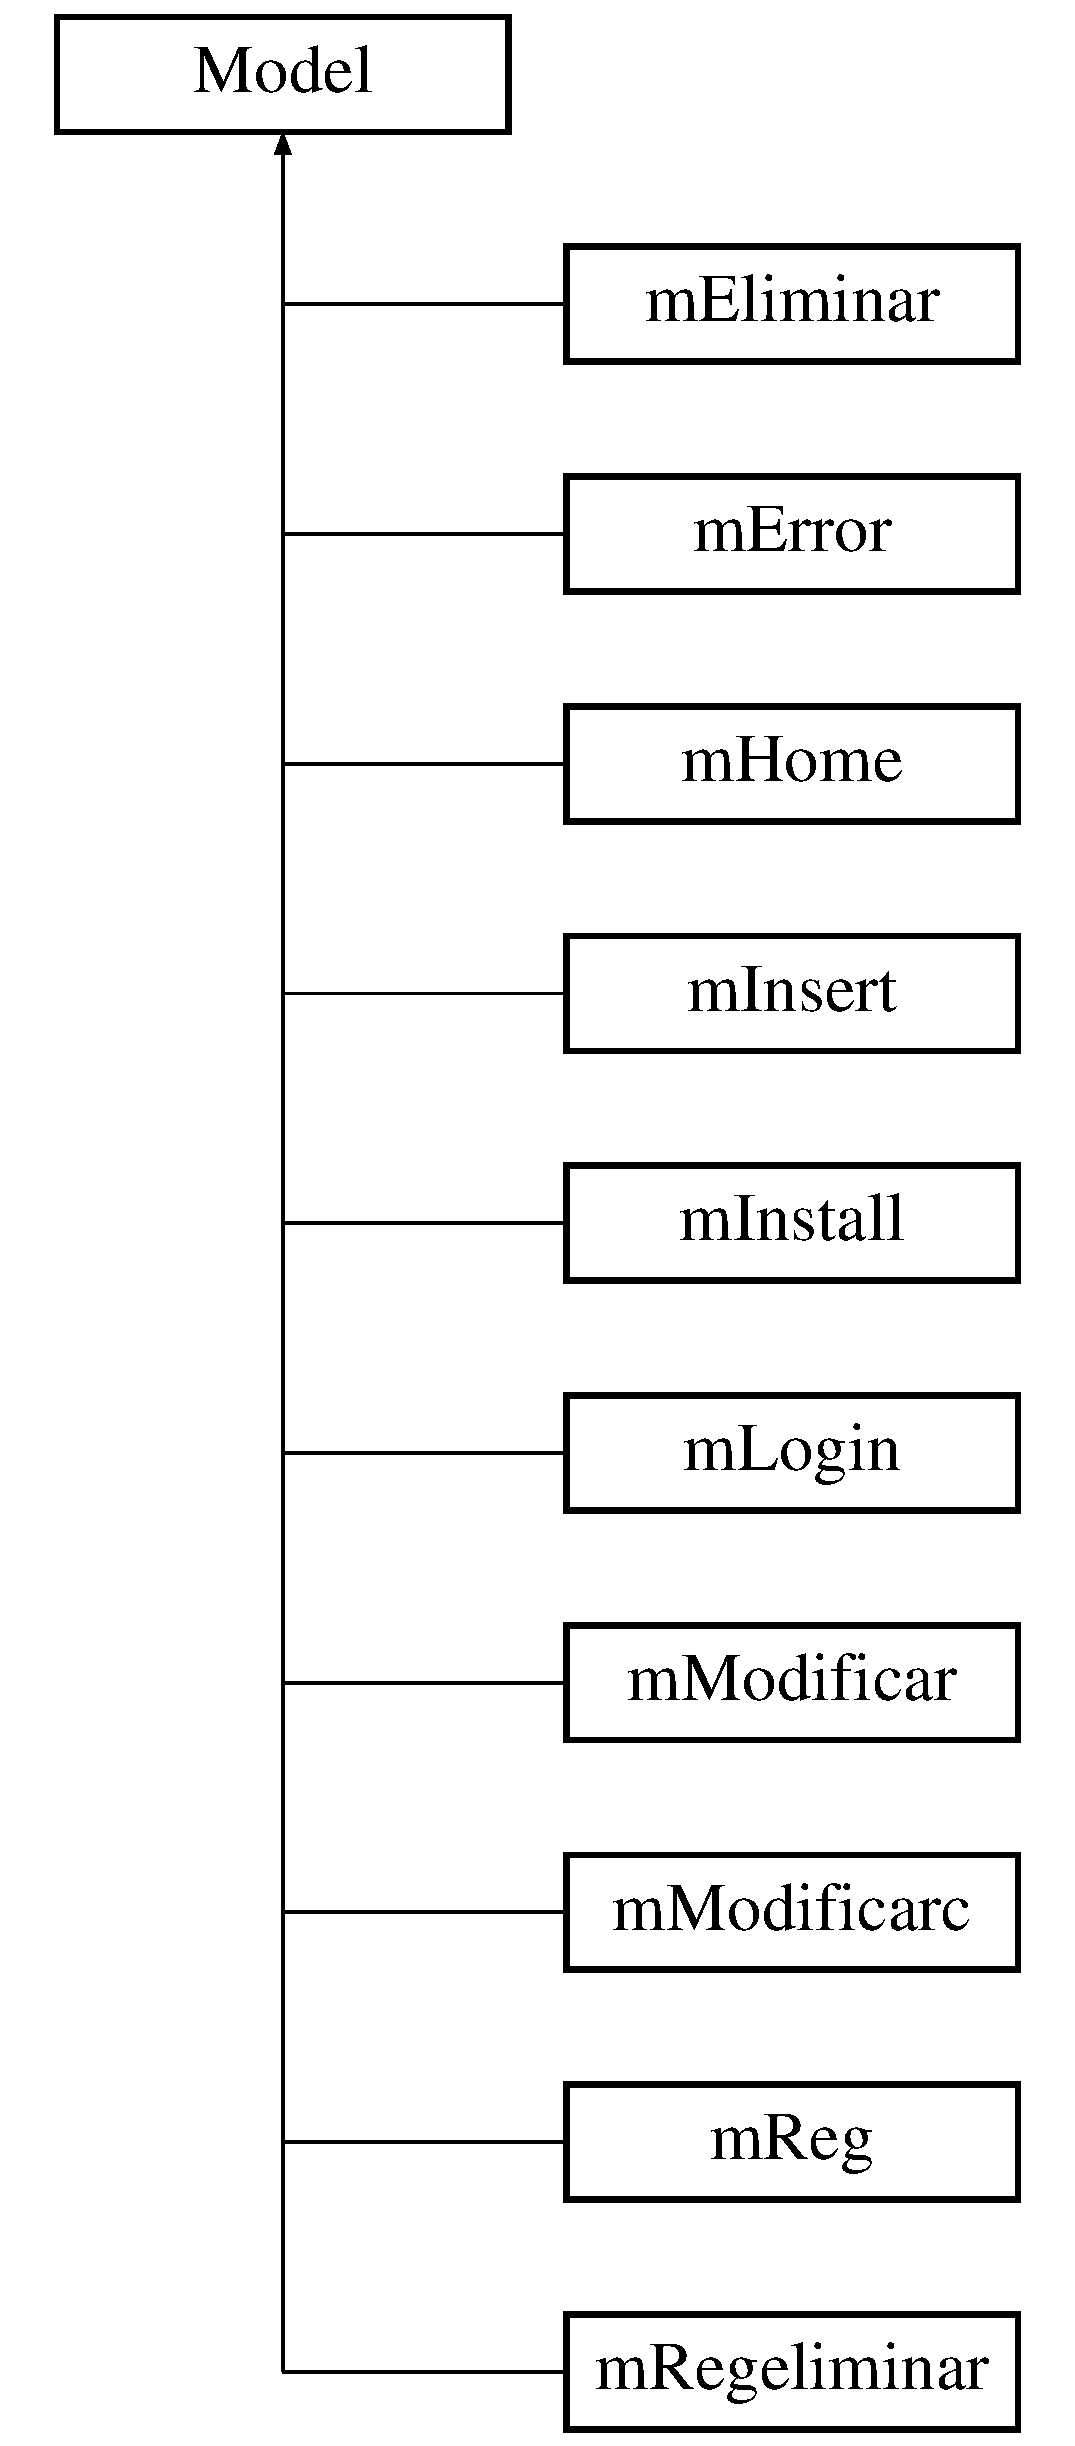
\includegraphics[height=11.000000cm]{class_model}
\end{center}
\end{figure}
\subsection*{Métodos públicos}
\begin{DoxyCompactItemize}
\item 
\hypertarget{class_model_a05014738840640fff5d40cc0604cb5c9}{}{\bfseries \+\_\+\+\_\+construct} (\$params=null)\label{class_model_a05014738840640fff5d40cc0604cb5c9}

\end{DoxyCompactItemize}
\subsection*{Atributos protegidos}
\begin{DoxyCompactItemize}
\item 
\hypertarget{class_model_a1fa3127fc82f96b1436d871ef02be319}{}{\bfseries \$db}\label{class_model_a1fa3127fc82f96b1436d871ef02be319}

\item 
\hypertarget{class_model_a8586c72f15bcedb0c9654f311323dde8}{}{\bfseries \$params\+\_\+in}\label{class_model_a8586c72f15bcedb0c9654f311323dde8}

\item 
\hypertarget{class_model_a25a8fffc5cc934f9cacb4f0aa27d5512}{}{\bfseries \$data\+\_\+out}\label{class_model_a25a8fffc5cc934f9cacb4f0aa27d5512}

\item 
\hypertarget{class_model_ae4901046cc3e1deebf77ccc785384a78}{}{\bfseries \$conf}\label{class_model_ae4901046cc3e1deebf77ccc785384a78}

\end{DoxyCompactItemize}


La documentación para esta clase fue generada a partir del siguiente fichero\+:\begin{DoxyCompactItemize}
\item 
sys/model.\+php\end{DoxyCompactItemize}

\hypertarget{class_modificar}{}\section{Referencia de la Clase Modificar}
\label{class_modificar}\index{Modificar@{Modificar}}
Diagrama de herencias de Modificar\begin{figure}[H]
\begin{center}
\leavevmode
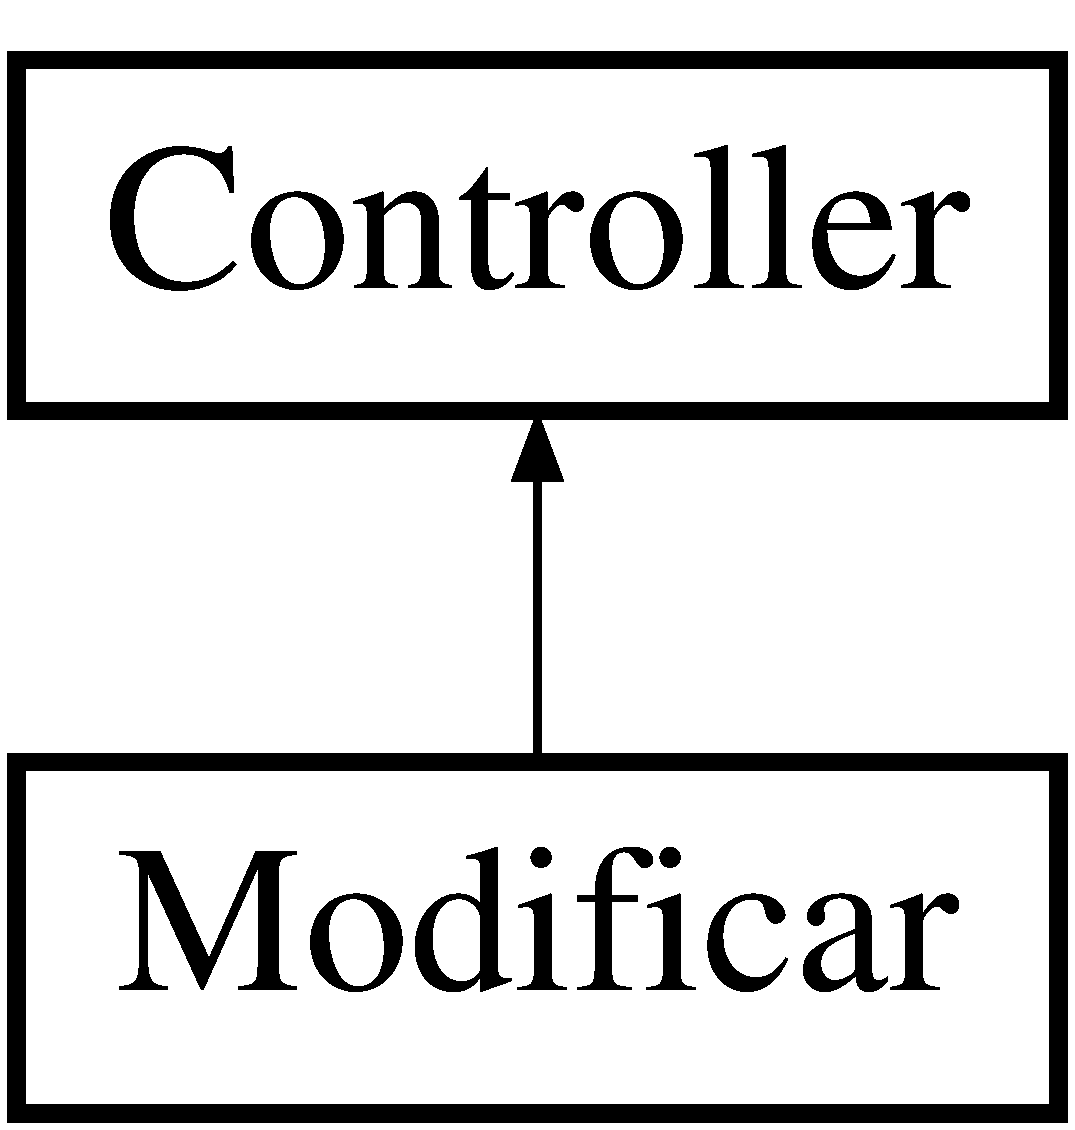
\includegraphics[height=2.000000cm]{class_modificar}
\end{center}
\end{figure}
\subsection*{Métodos públicos}
\begin{DoxyCompactItemize}
\item 
\hypertarget{class_modificar_a9162320adff1a1a4afd7f2372f753a3e}{}{\bfseries \+\_\+\+\_\+construct} (\$params)\label{class_modificar_a9162320adff1a1a4afd7f2372f753a3e}

\item 
\hypertarget{class_modificar_a174b8e4c7d4d7363c6f773671defdeff}{}{\bfseries home} ()\label{class_modificar_a174b8e4c7d4d7363c6f773671defdeff}

\item 
\hypertarget{class_modificar_aead84a6ded09739cf40826da2c341900}{}{\bfseries modificarusuario} ()\label{class_modificar_aead84a6ded09739cf40826da2c341900}

\item 
\hypertarget{class_modificar_aa744e58e4ea550a061a2e204f5126a71}{}{\bfseries modificar} ()\label{class_modificar_aa744e58e4ea550a061a2e204f5126a71}

\end{DoxyCompactItemize}
\subsection*{Otros miembros heredados}


La documentación para esta clase fue generada a partir del siguiente fichero\+:\begin{DoxyCompactItemize}
\item 
app/controllers/modificar.\+php\end{DoxyCompactItemize}

\hypertarget{class_modificarc}{}\section{Referencia de la Clase Modificarc}
\label{class_modificarc}\index{Modificarc@{Modificarc}}
Diagrama de herencias de Modificarc\begin{figure}[H]
\begin{center}
\leavevmode
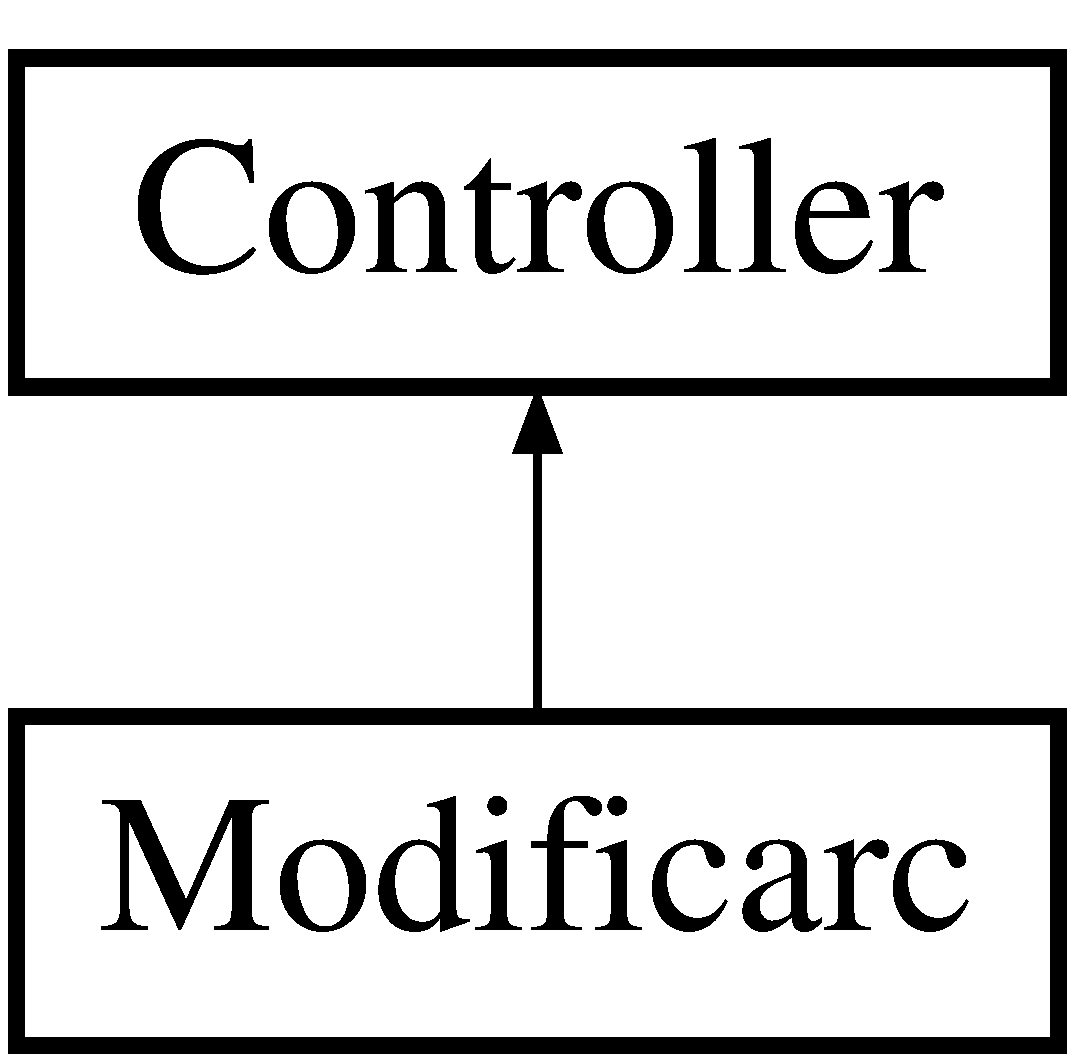
\includegraphics[height=2.000000cm]{class_modificarc}
\end{center}
\end{figure}
\subsection*{Métodos públicos}
\begin{DoxyCompactItemize}
\item 
\hypertarget{class_modificarc_a174b8e4c7d4d7363c6f773671defdeff}{}{\bfseries home} ()\label{class_modificarc_a174b8e4c7d4d7363c6f773671defdeff}

\end{DoxyCompactItemize}
\subsection*{Otros miembros heredados}


La documentación para esta clase fue generada a partir del siguiente fichero\+:\begin{DoxyCompactItemize}
\item 
app/controllers/modificarc.\+php\end{DoxyCompactItemize}

\hypertarget{classm_reg}{}\section{Referencia de la Clase m\+Reg}
\label{classm_reg}\index{m\+Reg@{m\+Reg}}
Diagrama de herencias de m\+Reg\begin{figure}[H]
\begin{center}
\leavevmode
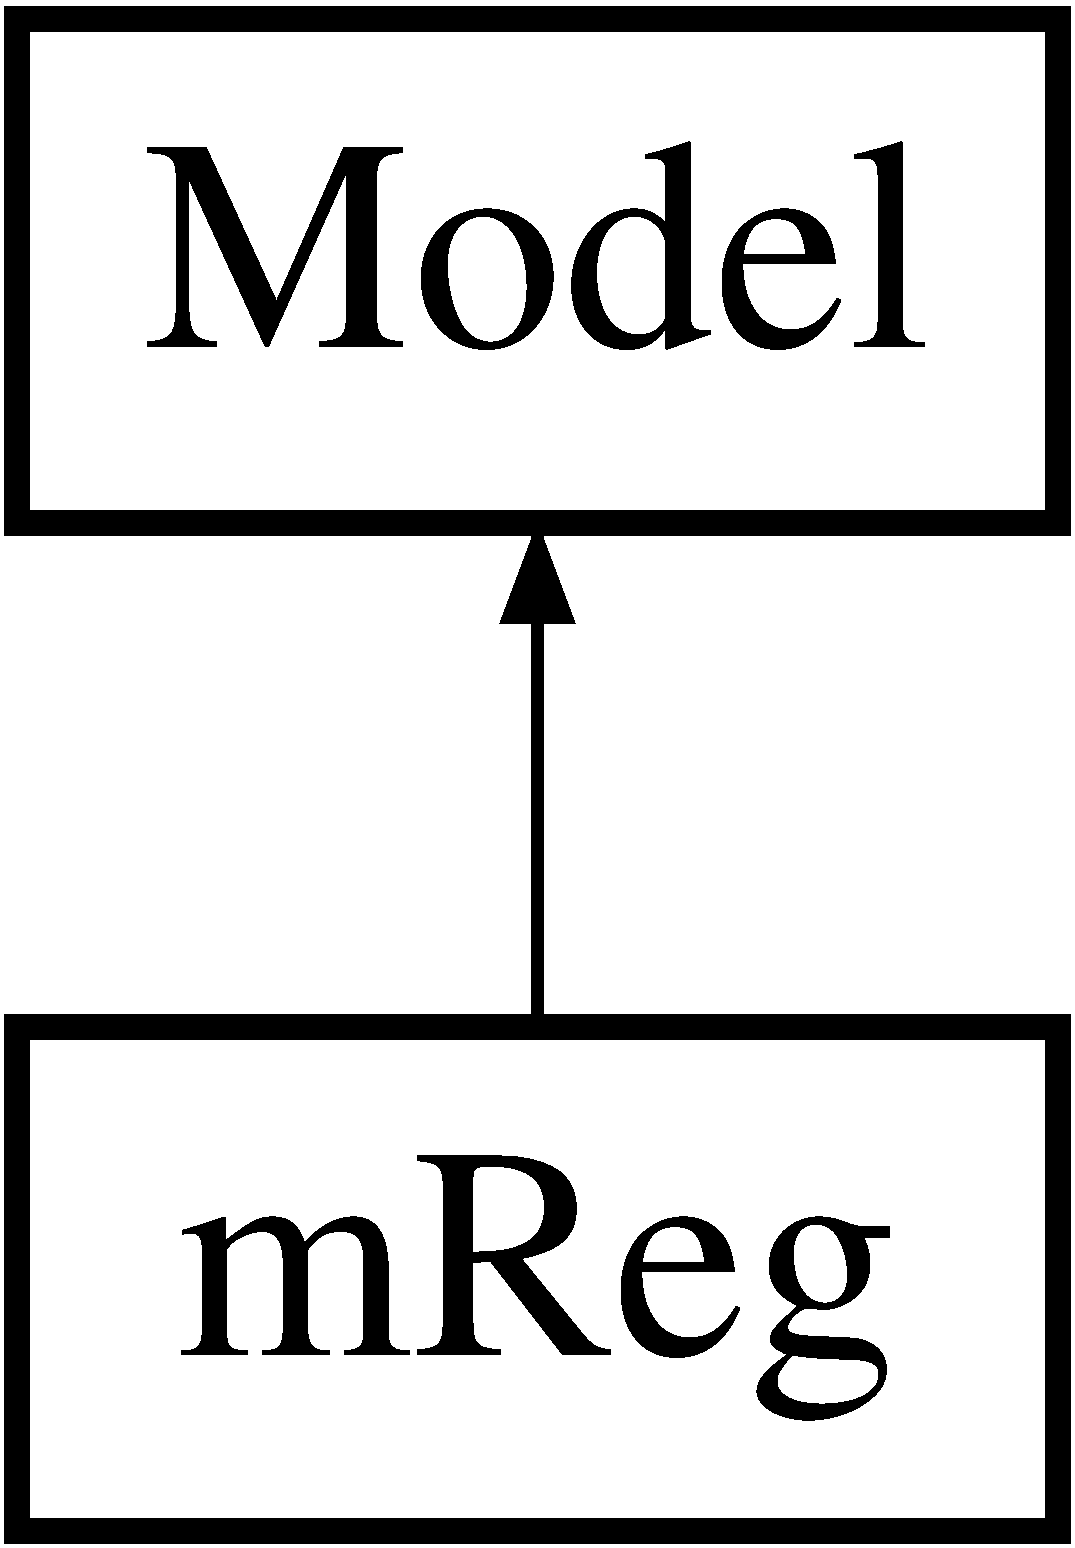
\includegraphics[height=2.000000cm]{classm_reg}
\end{center}
\end{figure}
\subsection*{Otros miembros heredados}


La documentación para esta clase fue generada a partir del siguiente fichero\+:\begin{DoxyCompactItemize}
\item 
app/models/mreg.\+php\end{DoxyCompactItemize}

\hypertarget{classm_regeliminar}{}\section{Referencia de la Clase m\+Regeliminar}
\label{classm_regeliminar}\index{m\+Regeliminar@{m\+Regeliminar}}
Diagrama de herencias de m\+Regeliminar\begin{figure}[H]
\begin{center}
\leavevmode
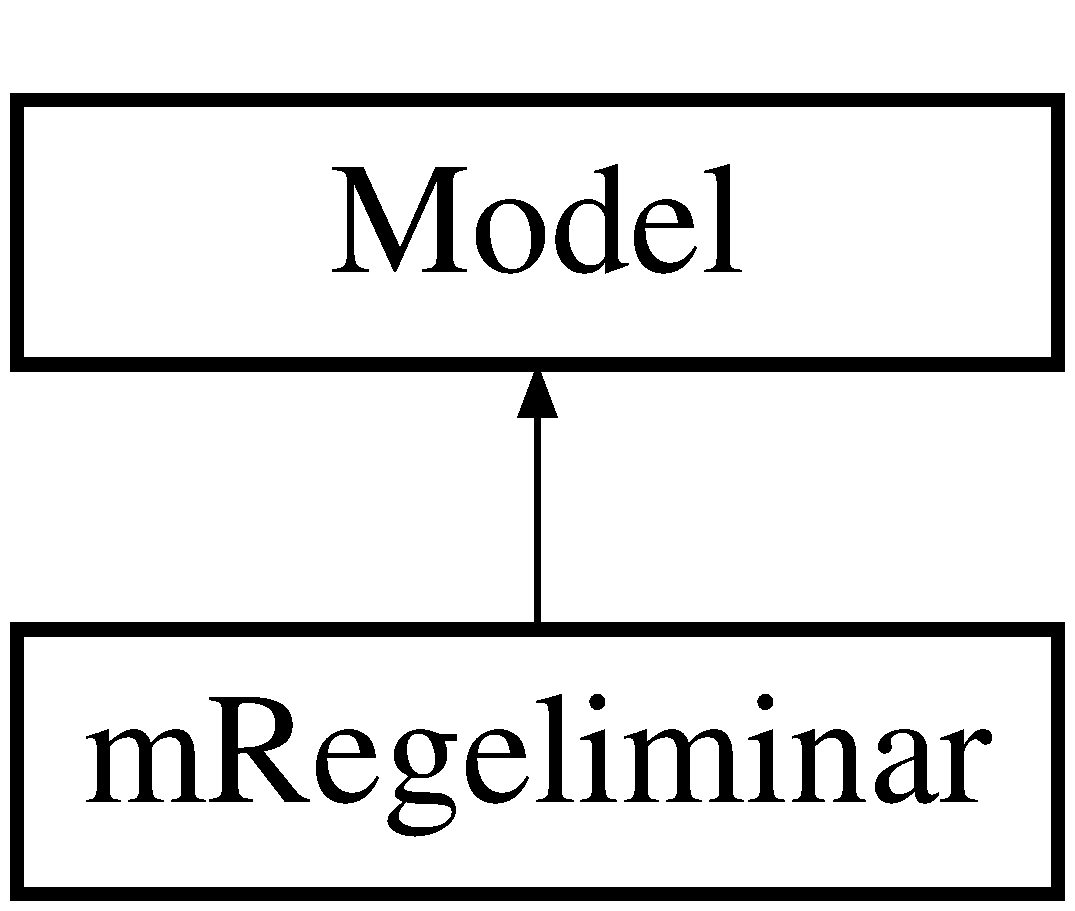
\includegraphics[height=2.000000cm]{classm_regeliminar}
\end{center}
\end{figure}
\subsection*{Otros miembros heredados}


La documentación para esta clase fue generada a partir del siguiente fichero\+:\begin{DoxyCompactItemize}
\item 
app/models/mregeliminar.\+php\end{DoxyCompactItemize}

\hypertarget{class_reg}{}\section{Referencia de la Clase Reg}
\label{class_reg}\index{Reg@{Reg}}
Diagrama de herencias de Reg\begin{figure}[H]
\begin{center}
\leavevmode
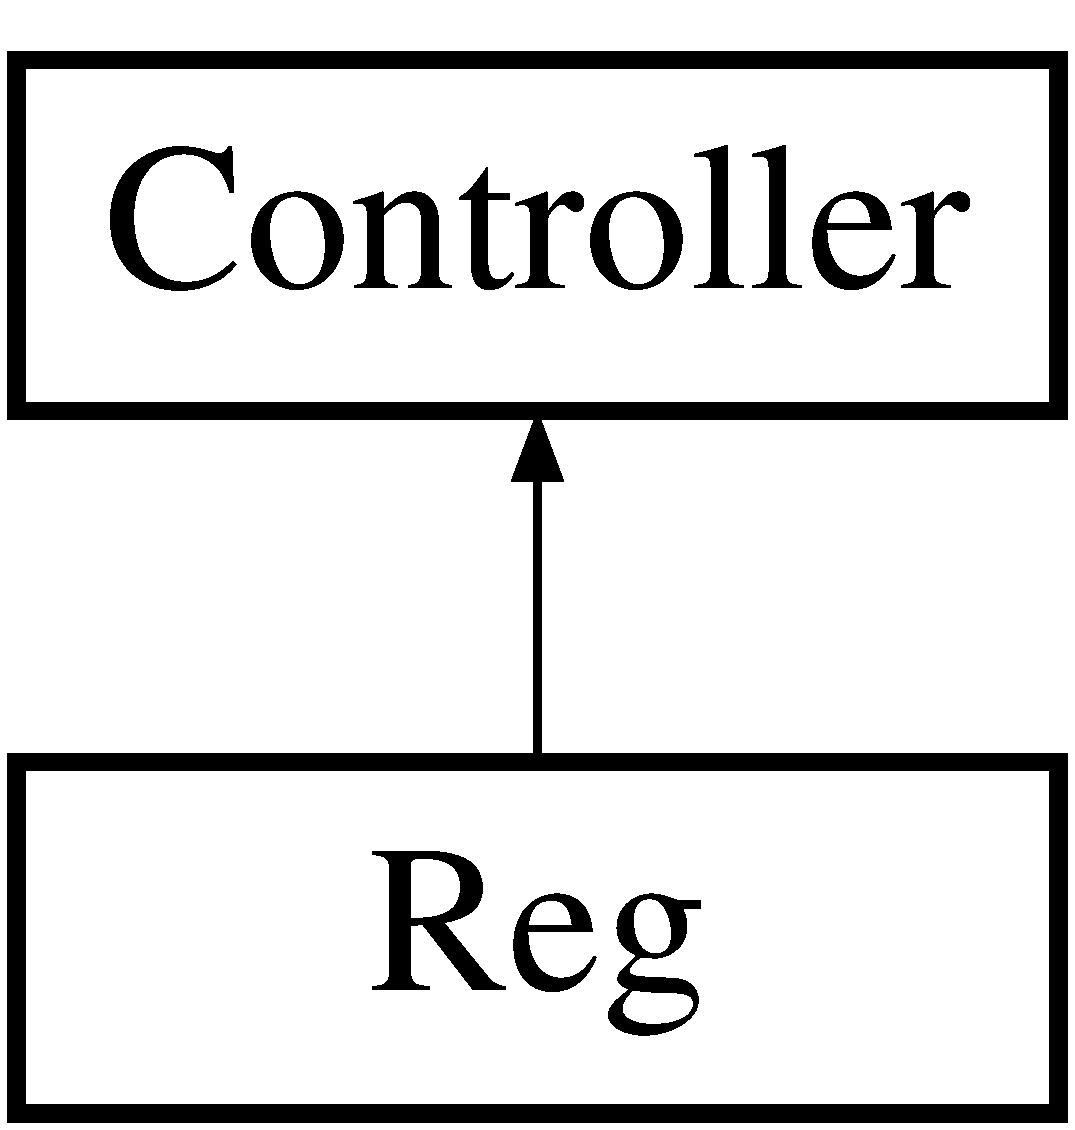
\includegraphics[height=2.000000cm]{class_reg}
\end{center}
\end{figure}
\subsection*{Métodos públicos}
\begin{DoxyCompactItemize}
\item 
\hypertarget{class_reg_a174b8e4c7d4d7363c6f773671defdeff}{}{\bfseries home} ()\label{class_reg_a174b8e4c7d4d7363c6f773671defdeff}

\end{DoxyCompactItemize}
\subsection*{Otros miembros heredados}


La documentación para esta clase fue generada a partir del siguiente fichero\+:\begin{DoxyCompactItemize}
\item 
app/controllers/reg.\+php\end{DoxyCompactItemize}

\hypertarget{class_regeliminar}{}\section{Referencia de la Clase Regeliminar}
\label{class_regeliminar}\index{Regeliminar@{Regeliminar}}
Diagrama de herencias de Regeliminar\begin{figure}[H]
\begin{center}
\leavevmode
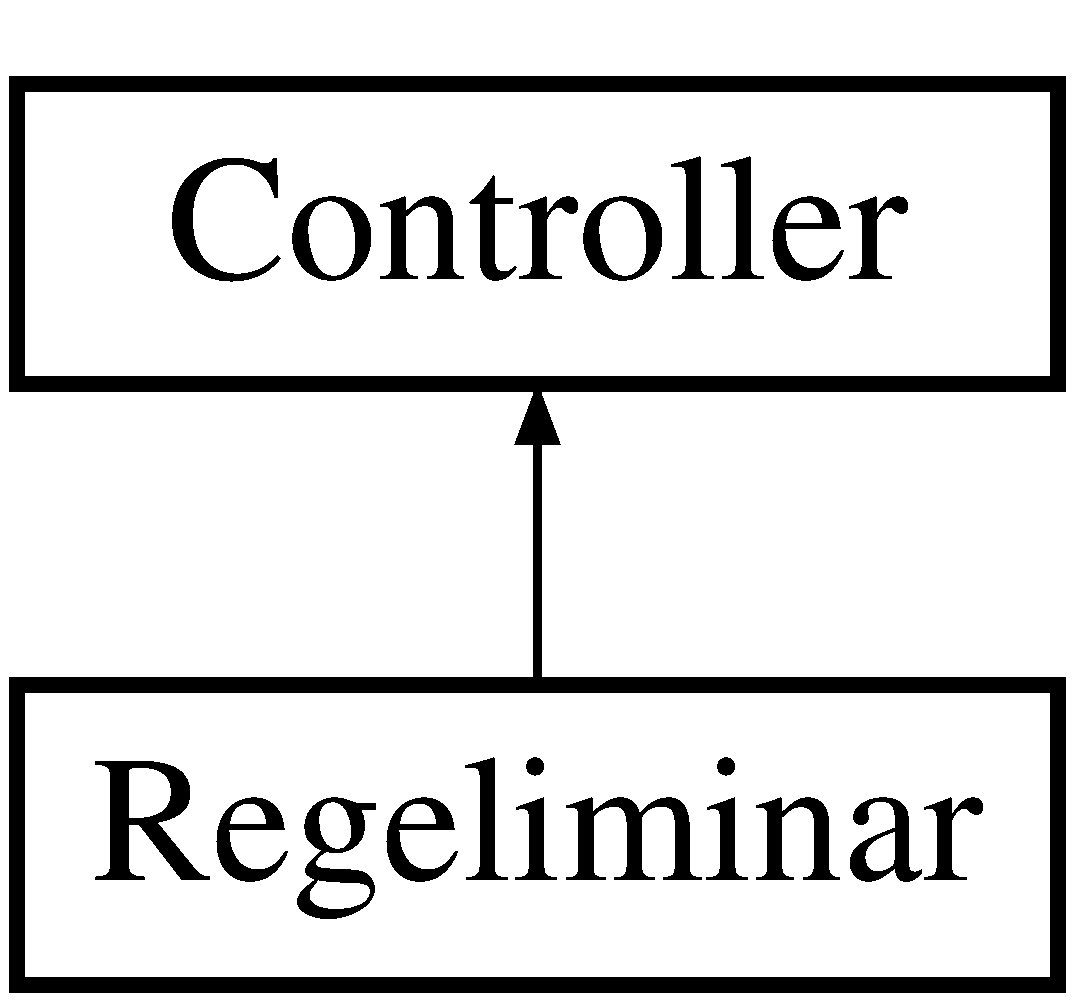
\includegraphics[height=2.000000cm]{class_regeliminar}
\end{center}
\end{figure}
\subsection*{Métodos públicos}
\begin{DoxyCompactItemize}
\item 
\hypertarget{class_regeliminar_a174b8e4c7d4d7363c6f773671defdeff}{}{\bfseries home} ()\label{class_regeliminar_a174b8e4c7d4d7363c6f773671defdeff}

\end{DoxyCompactItemize}
\subsection*{Otros miembros heredados}


La documentación para esta clase fue generada a partir del siguiente fichero\+:\begin{DoxyCompactItemize}
\item 
app/controllers/regeliminar.\+php\end{DoxyCompactItemize}

\hypertarget{class_registry}{}\section{Referencia de la Clase Registry}
\label{class_registry}\index{Registry@{Registry}}
\subsection*{Métodos públicos}
\begin{DoxyCompactItemize}
\item 
\hypertarget{class_registry_aa2c6e0f52eebf99a2bb4b6ba88d7b156}{}{\bfseries \+\_\+\+\_\+set} (\$key, \$var)\label{class_registry_aa2c6e0f52eebf99a2bb4b6ba88d7b156}

\item 
\hypertarget{class_registry_a4537dad3b44254124991341cc91b28fb}{}{\bfseries \+\_\+\+\_\+get} (\$key)\label{class_registry_a4537dad3b44254124991341cc91b28fb}

\item 
\hypertarget{class_registry_ab8c29e72070f8e32d1a5119fb708e5e3}{}{\bfseries \+\_\+\+\_\+unset} (\$data)\label{class_registry_ab8c29e72070f8e32d1a5119fb708e5e3}

\item 
\hypertarget{class_registry_a81a67162a6288d78fc4c55283325f0b4}{}{\bfseries get\+Data} ()\label{class_registry_a81a67162a6288d78fc4c55283325f0b4}

\item 
\hypertarget{class_registry_a4be4055f3361d4800e16bc2e2e38cda6}{}{\bfseries init} ()\label{class_registry_a4be4055f3361d4800e16bc2e2e38cda6}

\end{DoxyCompactItemize}
\subsection*{Métodos públicos estáticos}
\begin{DoxyCompactItemize}
\item 
\hypertarget{class_registry_ac93fbec81f07e5d15f80db907e63dc10}{}static {\bfseries get\+Instance} ()\label{class_registry_ac93fbec81f07e5d15f80db907e63dc10}

\end{DoxyCompactItemize}
\subsection*{Atributos públicos estáticos}
\begin{DoxyCompactItemize}
\item 
\hypertarget{class_registry_ad9d7ce33ebb142b70e58b68052ca0ea8}{}static {\bfseries \$instance}\label{class_registry_ad9d7ce33ebb142b70e58b68052ca0ea8}

\end{DoxyCompactItemize}


La documentación para esta clase fue generada a partir del siguiente fichero\+:\begin{DoxyCompactItemize}
\item 
sys/registry.\+php\end{DoxyCompactItemize}

\hypertarget{class_request}{}\section{Referencia de la Clase Request}
\label{class_request}\index{Request@{Request}}
\subsection*{Métodos públicos estáticos}
\begin{DoxyCompactItemize}
\item 
\hypertarget{class_request_ad7c00fdbba951c6f593e1e81f83a9324}{}static {\bfseries retrieve} ()\label{class_request_ad7c00fdbba951c6f593e1e81f83a9324}

\item 
\hypertarget{class_request_a757eb52465094807a57e1604193c3957}{}static {\bfseries get\+Cont} ()\label{class_request_a757eb52465094807a57e1604193c3957}

\item 
\hypertarget{class_request_aa6d9c2b196225e95b4142166b936ef12}{}static {\bfseries get\+Act} ()\label{class_request_aa6d9c2b196225e95b4142166b936ef12}

\item 
\hypertarget{class_request_aff93c1546ca6a0a3a86cb21fab0ce5a5}{}static {\bfseries get\+Param} ()\label{class_request_aff93c1546ca6a0a3a86cb21fab0ce5a5}

\end{DoxyCompactItemize}


La documentación para esta clase fue generada a partir del siguiente fichero\+:\begin{DoxyCompactItemize}
\item 
sys/request.\+php\end{DoxyCompactItemize}

\hypertarget{class_session}{}\section{Referencia de la Clase Session}
\label{class_session}\index{Session@{Session}}
\subsection*{Métodos públicos}
\begin{DoxyCompactItemize}
\item 
\hypertarget{class_session_a630ed254117528083a87c0e30f1e8eab}{}{\bfseries save\+\_\+session} (\$db)\label{class_session_a630ed254117528083a87c0e30f1e8eab}

\item 
\hypertarget{class_session_a79b36d71c6f1d4f9e6c4c3e34c081456}{}{\bfseries \+\_\+\+\_\+set} (\$key, \$value)\label{class_session_a79b36d71c6f1d4f9e6c4c3e34c081456}

\item 
\hypertarget{class_session_a4537dad3b44254124991341cc91b28fb}{}{\bfseries \+\_\+\+\_\+get} (\$key)\label{class_session_a4537dad3b44254124991341cc91b28fb}

\end{DoxyCompactItemize}
\subsection*{Métodos públicos estáticos}
\begin{DoxyCompactItemize}
\item 
\hypertarget{class_session_a9f0be6ae273d3669e11c29910a0be338}{}static {\bfseries init} ()\label{class_session_a9f0be6ae273d3669e11c29910a0be338}

\item 
\hypertarget{class_session_a606e29124233412b3db261bb6078d4a0}{}static {\bfseries destroy} (\$key=false)\label{class_session_a606e29124233412b3db261bb6078d4a0}

\end{DoxyCompactItemize}
\subsection*{Atributos protegidos}
\begin{DoxyCompactItemize}
\item 
\hypertarget{class_session_a1fa3127fc82f96b1436d871ef02be319}{}{\bfseries \$db}\label{class_session_a1fa3127fc82f96b1436d871ef02be319}

\end{DoxyCompactItemize}


La documentación para esta clase fue generada a partir del siguiente fichero\+:\begin{DoxyCompactItemize}
\item 
sys/session.\+php\end{DoxyCompactItemize}

\hypertarget{class_s_q_l_parser}{}\section{Referencia de la Clase S\+Q\+L\+Parser}
\label{class_s_q_l_parser}\index{S\+Q\+L\+Parser@{S\+Q\+L\+Parser}}
\subsection*{Métodos públicos estáticos}
\begin{DoxyCompactItemize}
\item 
\hypertarget{class_s_q_l_parser_acb297d08abcd4ac4fabe1fbe54042e3d}{}static {\bfseries out\+Comments} (\$query)\label{class_s_q_l_parser_acb297d08abcd4ac4fabe1fbe54042e3d}

\item 
\hypertarget{class_s_q_l_parser_a6185a1ba348b3b151ba1c9a12f553508}{}static {\bfseries parse} (\$content)\label{class_s_q_l_parser_a6185a1ba348b3b151ba1c9a12f553508}

\end{DoxyCompactItemize}


La documentación para esta clase fue generada a partir del siguiente fichero\+:\begin{DoxyCompactItemize}
\item 
sys/helper.\+php\end{DoxyCompactItemize}

\hypertarget{class_template}{}\section{Referencia de la Clase Template}
\label{class_template}\index{Template@{Template}}
\subsection*{Métodos públicos estáticos}
\begin{DoxyCompactItemize}
\item 
\hypertarget{class_template_a58fdd5b502414a7db42dddfb3e0a1a6f}{}static {\bfseries load} (\$contents, \$data=null)\label{class_template_a58fdd5b502414a7db42dddfb3e0a1a6f}

\end{DoxyCompactItemize}


La documentación para esta clase fue generada a partir del siguiente fichero\+:\begin{DoxyCompactItemize}
\item 
sys/template.\+php\end{DoxyCompactItemize}

\hypertarget{classv_create}{}\section{Referencia de la Clase v\+Create}
\label{classv_create}\index{v\+Create@{v\+Create}}
Diagrama de herencias de v\+Create\begin{figure}[H]
\begin{center}
\leavevmode
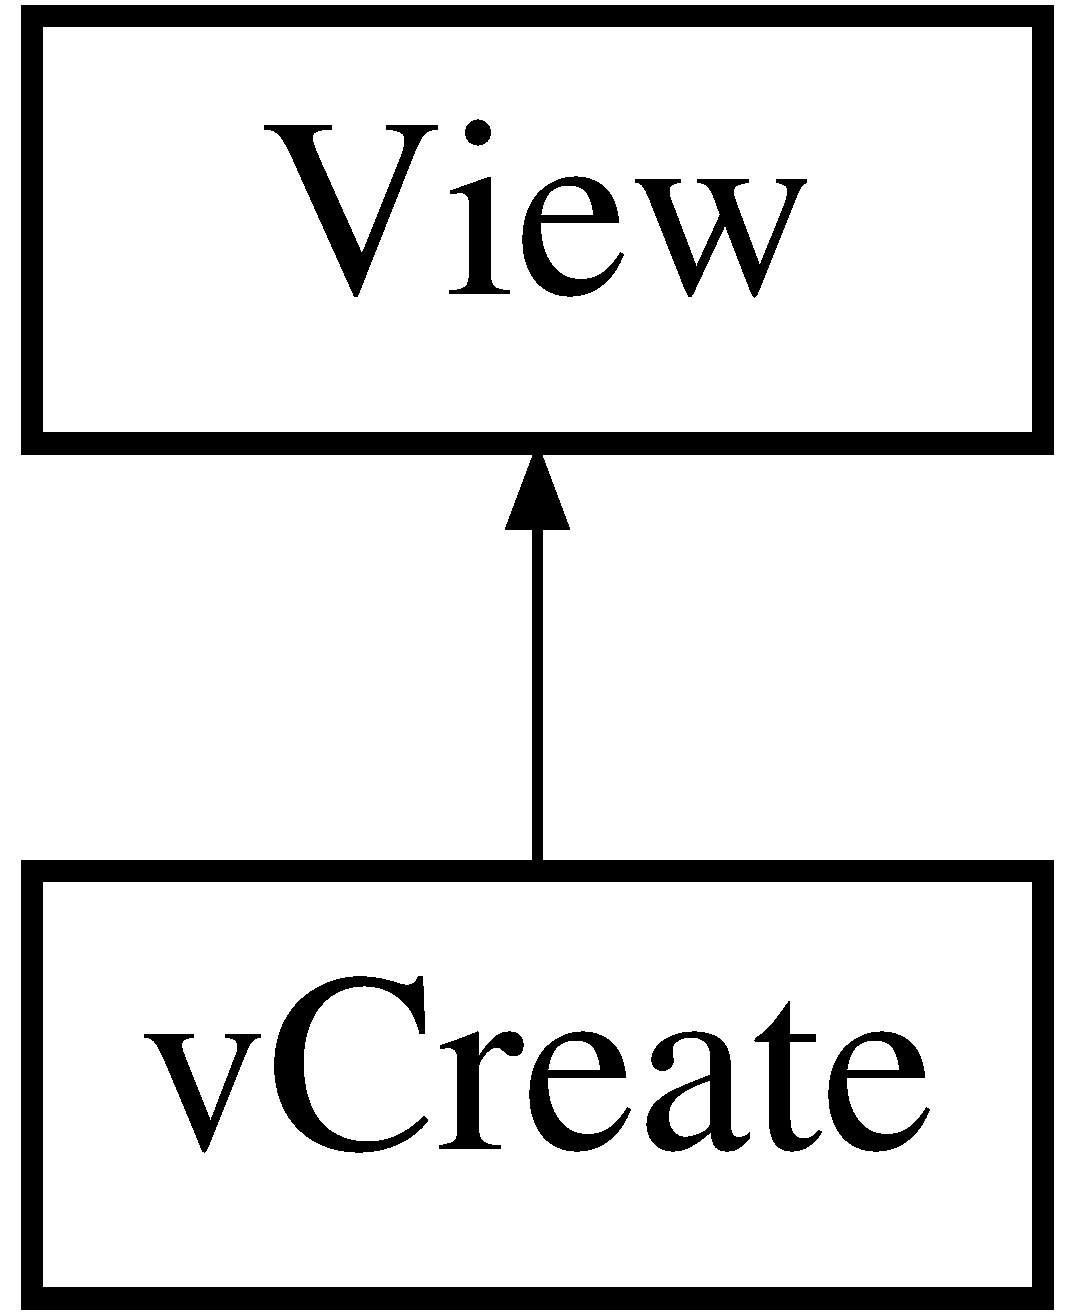
\includegraphics[height=2.000000cm]{classv_create}
\end{center}
\end{figure}
\subsection*{Otros miembros heredados}


La documentación para esta clase fue generada a partir del siguiente fichero\+:\begin{DoxyCompactItemize}
\item 
app/views/vcreate.\+php\end{DoxyCompactItemize}

\hypertarget{classv_eliminar}{}\section{Referencia de la Clase v\+Eliminar}
\label{classv_eliminar}\index{v\+Eliminar@{v\+Eliminar}}
Diagrama de herencias de v\+Eliminar\begin{figure}[H]
\begin{center}
\leavevmode
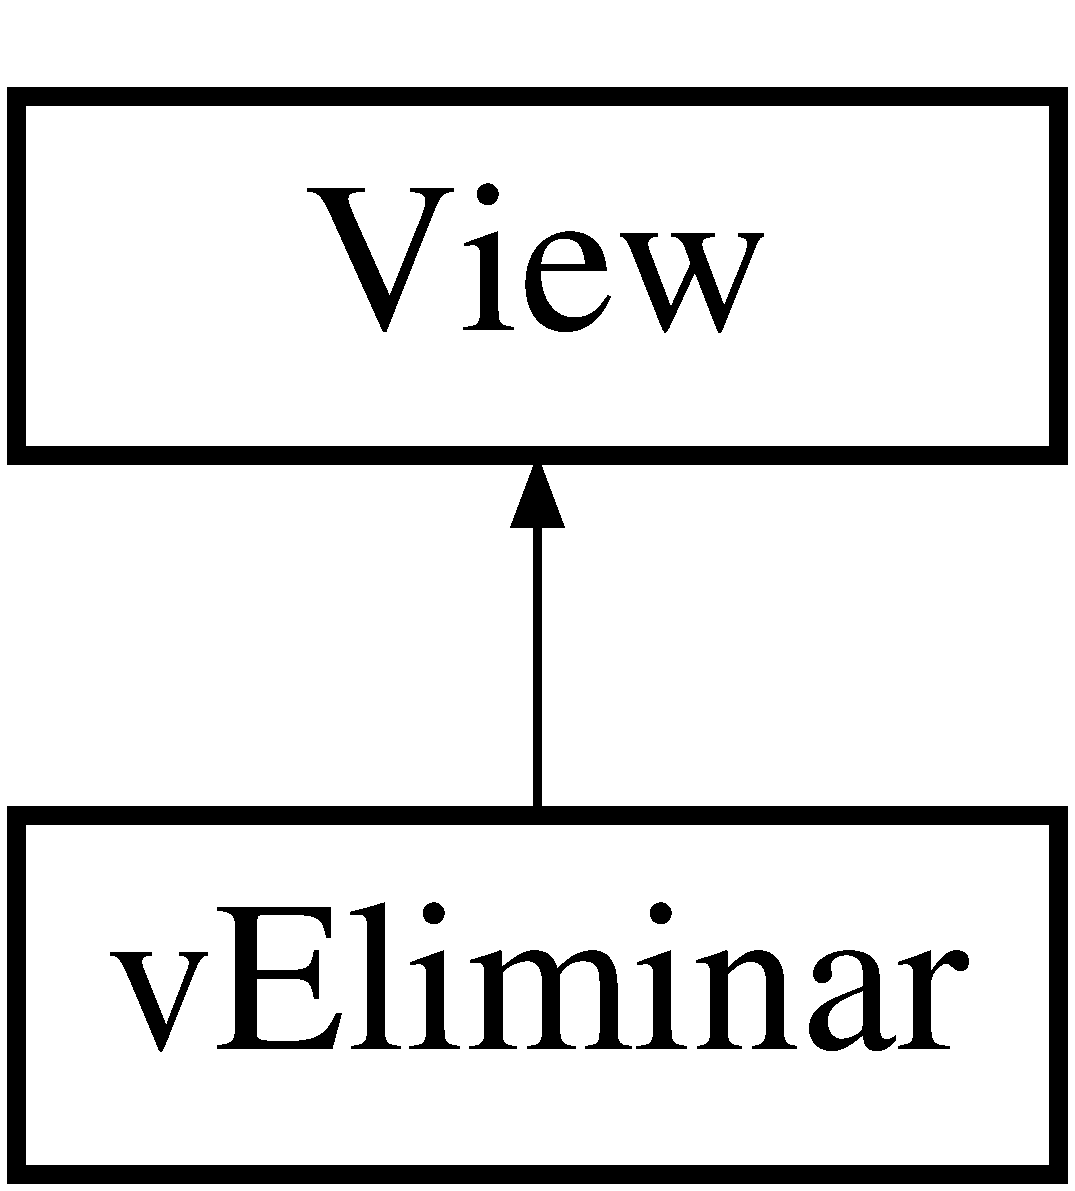
\includegraphics[height=2.000000cm]{classv_eliminar}
\end{center}
\end{figure}
\subsection*{Otros miembros heredados}


La documentación para esta clase fue generada a partir del siguiente fichero\+:\begin{DoxyCompactItemize}
\item 
app/views/veliminar.\+php\end{DoxyCompactItemize}

\hypertarget{classv_error}{}\section{Referencia de la Clase v\+Error}
\label{classv_error}\index{v\+Error@{v\+Error}}
Diagrama de herencias de v\+Error\begin{figure}[H]
\begin{center}
\leavevmode
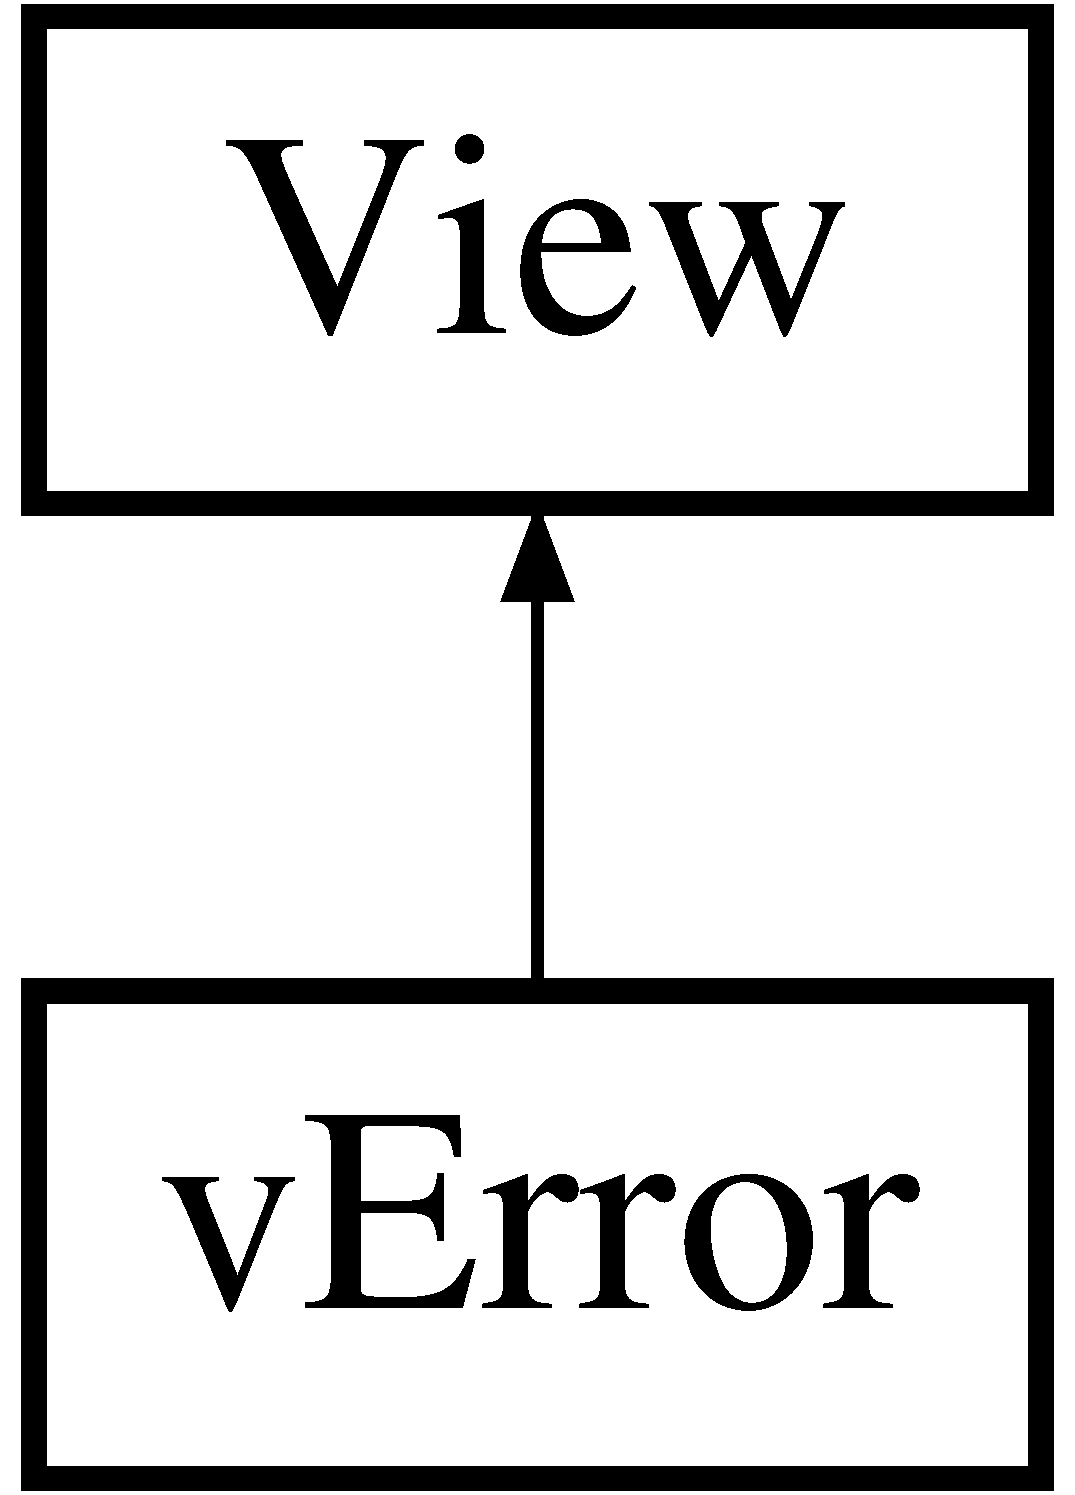
\includegraphics[height=2.000000cm]{classv_error}
\end{center}
\end{figure}
\subsection*{Otros miembros heredados}


La documentación para esta clase fue generada a partir del siguiente fichero\+:\begin{DoxyCompactItemize}
\item 
app/views/verror.\+php\end{DoxyCompactItemize}

\hypertarget{classv_errorcrear}{}\section{Referencia de la Clase v\+Errorcrear}
\label{classv_errorcrear}\index{v\+Errorcrear@{v\+Errorcrear}}
Diagrama de herencias de v\+Errorcrear\begin{figure}[H]
\begin{center}
\leavevmode
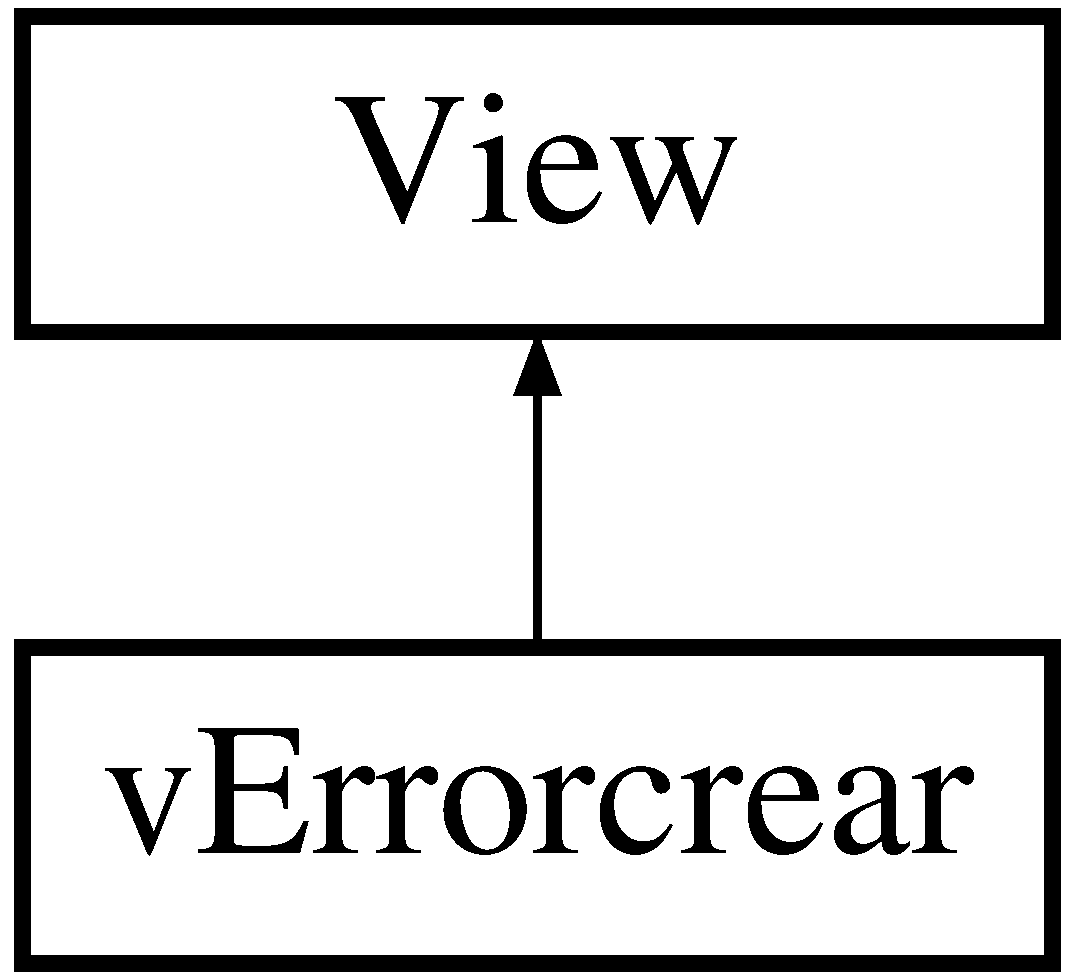
\includegraphics[height=2.000000cm]{classv_errorcrear}
\end{center}
\end{figure}
\subsection*{Otros miembros heredados}


La documentación para esta clase fue generada a partir del siguiente fichero\+:\begin{DoxyCompactItemize}
\item 
app/views/verrorcrear.\+php\end{DoxyCompactItemize}

\hypertarget{classv_erroreliminar}{}\section{Referencia de la Clase v\+Erroreliminar}
\label{classv_erroreliminar}\index{v\+Erroreliminar@{v\+Erroreliminar}}
Diagrama de herencias de v\+Erroreliminar\begin{figure}[H]
\begin{center}
\leavevmode
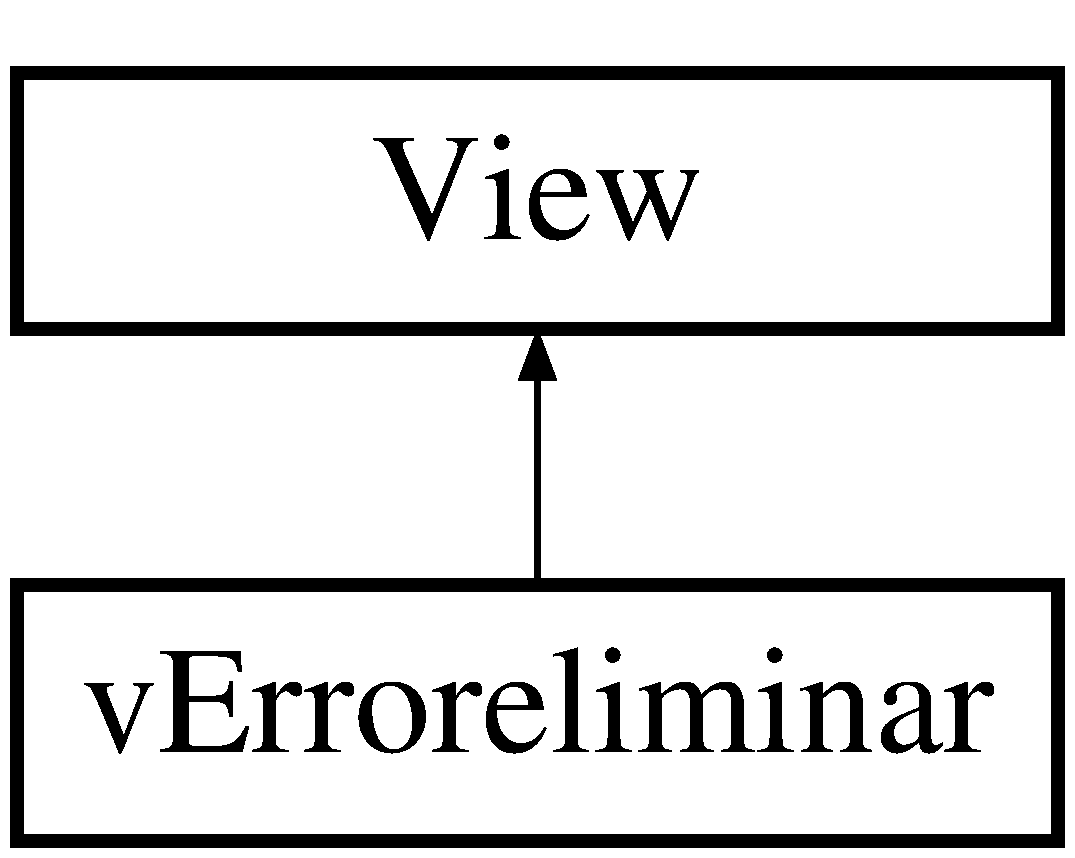
\includegraphics[height=2.000000cm]{classv_erroreliminar}
\end{center}
\end{figure}
\subsection*{Otros miembros heredados}


La documentación para esta clase fue generada a partir del siguiente fichero\+:\begin{DoxyCompactItemize}
\item 
app/views/verroreliminar.\+php\end{DoxyCompactItemize}

\hypertarget{classv_errorlogin}{}\section{Referencia de la Clase v\+Errorlogin}
\label{classv_errorlogin}\index{v\+Errorlogin@{v\+Errorlogin}}
Diagrama de herencias de v\+Errorlogin\begin{figure}[H]
\begin{center}
\leavevmode
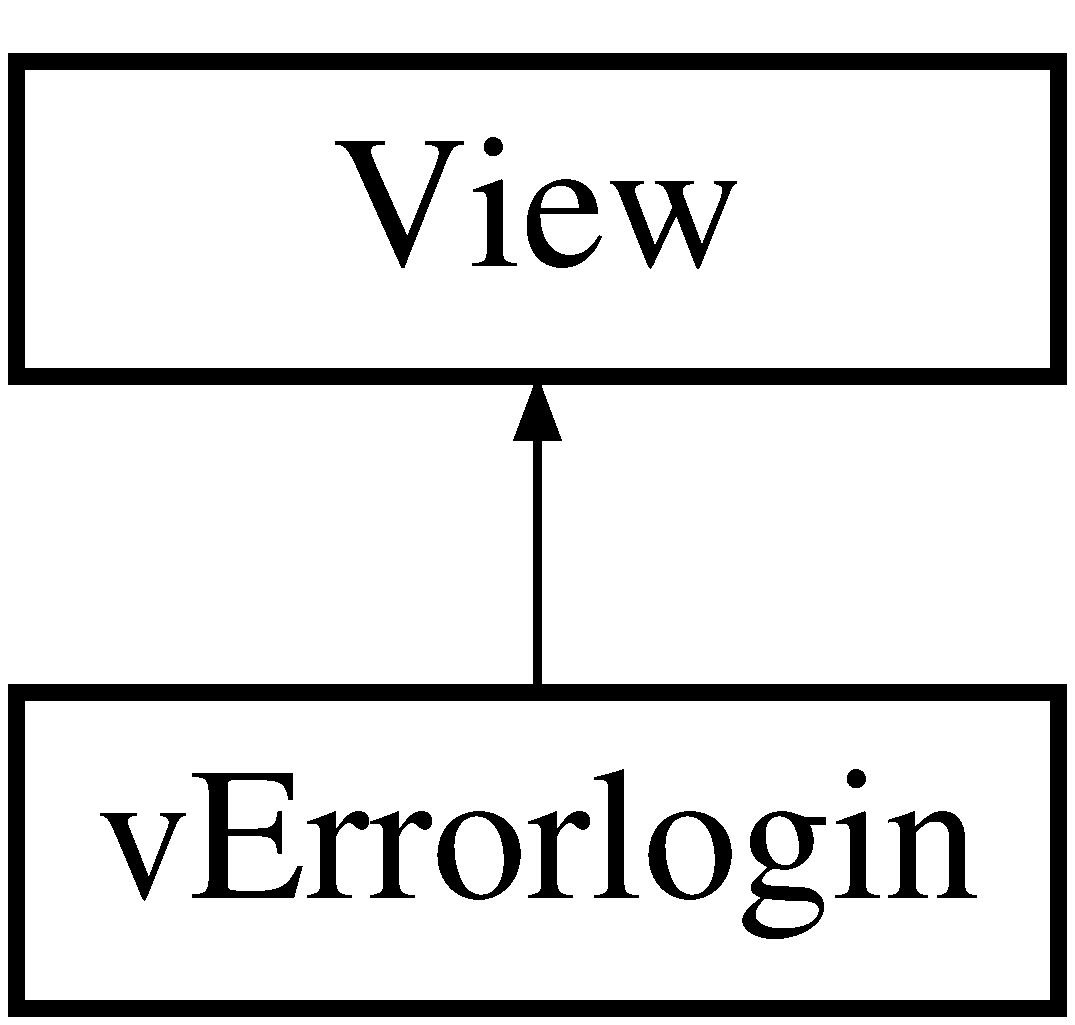
\includegraphics[height=2.000000cm]{classv_errorlogin}
\end{center}
\end{figure}
\subsection*{Otros miembros heredados}


La documentación para esta clase fue generada a partir del siguiente fichero\+:\begin{DoxyCompactItemize}
\item 
app/views/verrorlogin.\+php\end{DoxyCompactItemize}

\hypertarget{classv_errormodificar}{}\section{Referencia de la Clase v\+Errormodificar}
\label{classv_errormodificar}\index{v\+Errormodificar@{v\+Errormodificar}}
Diagrama de herencias de v\+Errormodificar\begin{figure}[H]
\begin{center}
\leavevmode
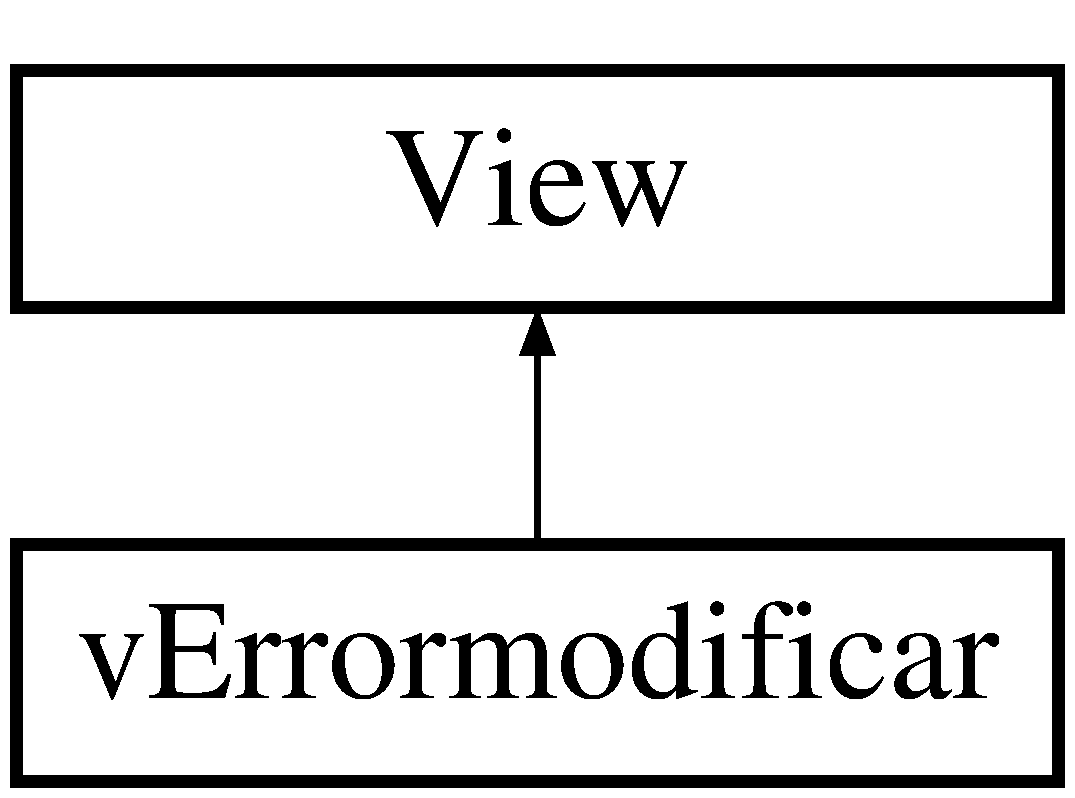
\includegraphics[height=2.000000cm]{classv_errormodificar}
\end{center}
\end{figure}
\subsection*{Otros miembros heredados}


La documentación para esta clase fue generada a partir del siguiente fichero\+:\begin{DoxyCompactItemize}
\item 
app/views/verrormodificar.\+php\end{DoxyCompactItemize}

\hypertarget{classv_home}{}\section{Referencia de la Clase v\+Home}
\label{classv_home}\index{v\+Home@{v\+Home}}
Diagrama de herencias de v\+Home\begin{figure}[H]
\begin{center}
\leavevmode
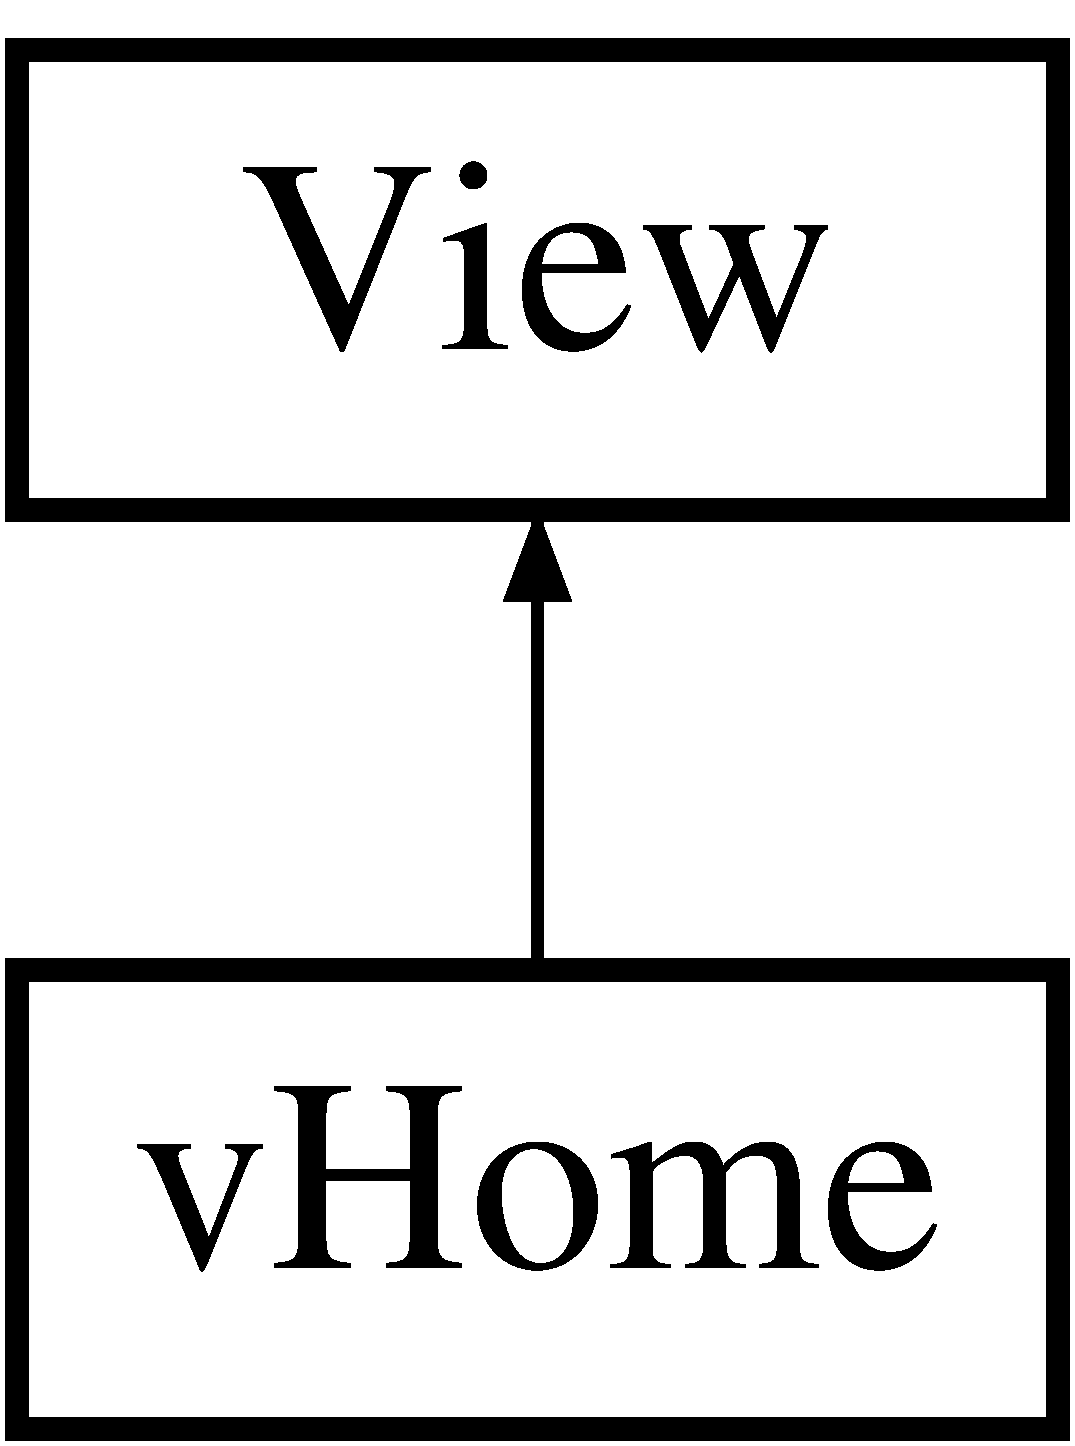
\includegraphics[height=2.000000cm]{classv_home}
\end{center}
\end{figure}
\subsection*{Otros miembros heredados}


La documentación para esta clase fue generada a partir del siguiente fichero\+:\begin{DoxyCompactItemize}
\item 
app/views/vhome.\+php\end{DoxyCompactItemize}

\hypertarget{class_view}{}\section{Referencia de la Clase View}
\label{class_view}\index{View@{View}}
Diagrama de herencias de View\begin{figure}[H]
\begin{center}
\leavevmode
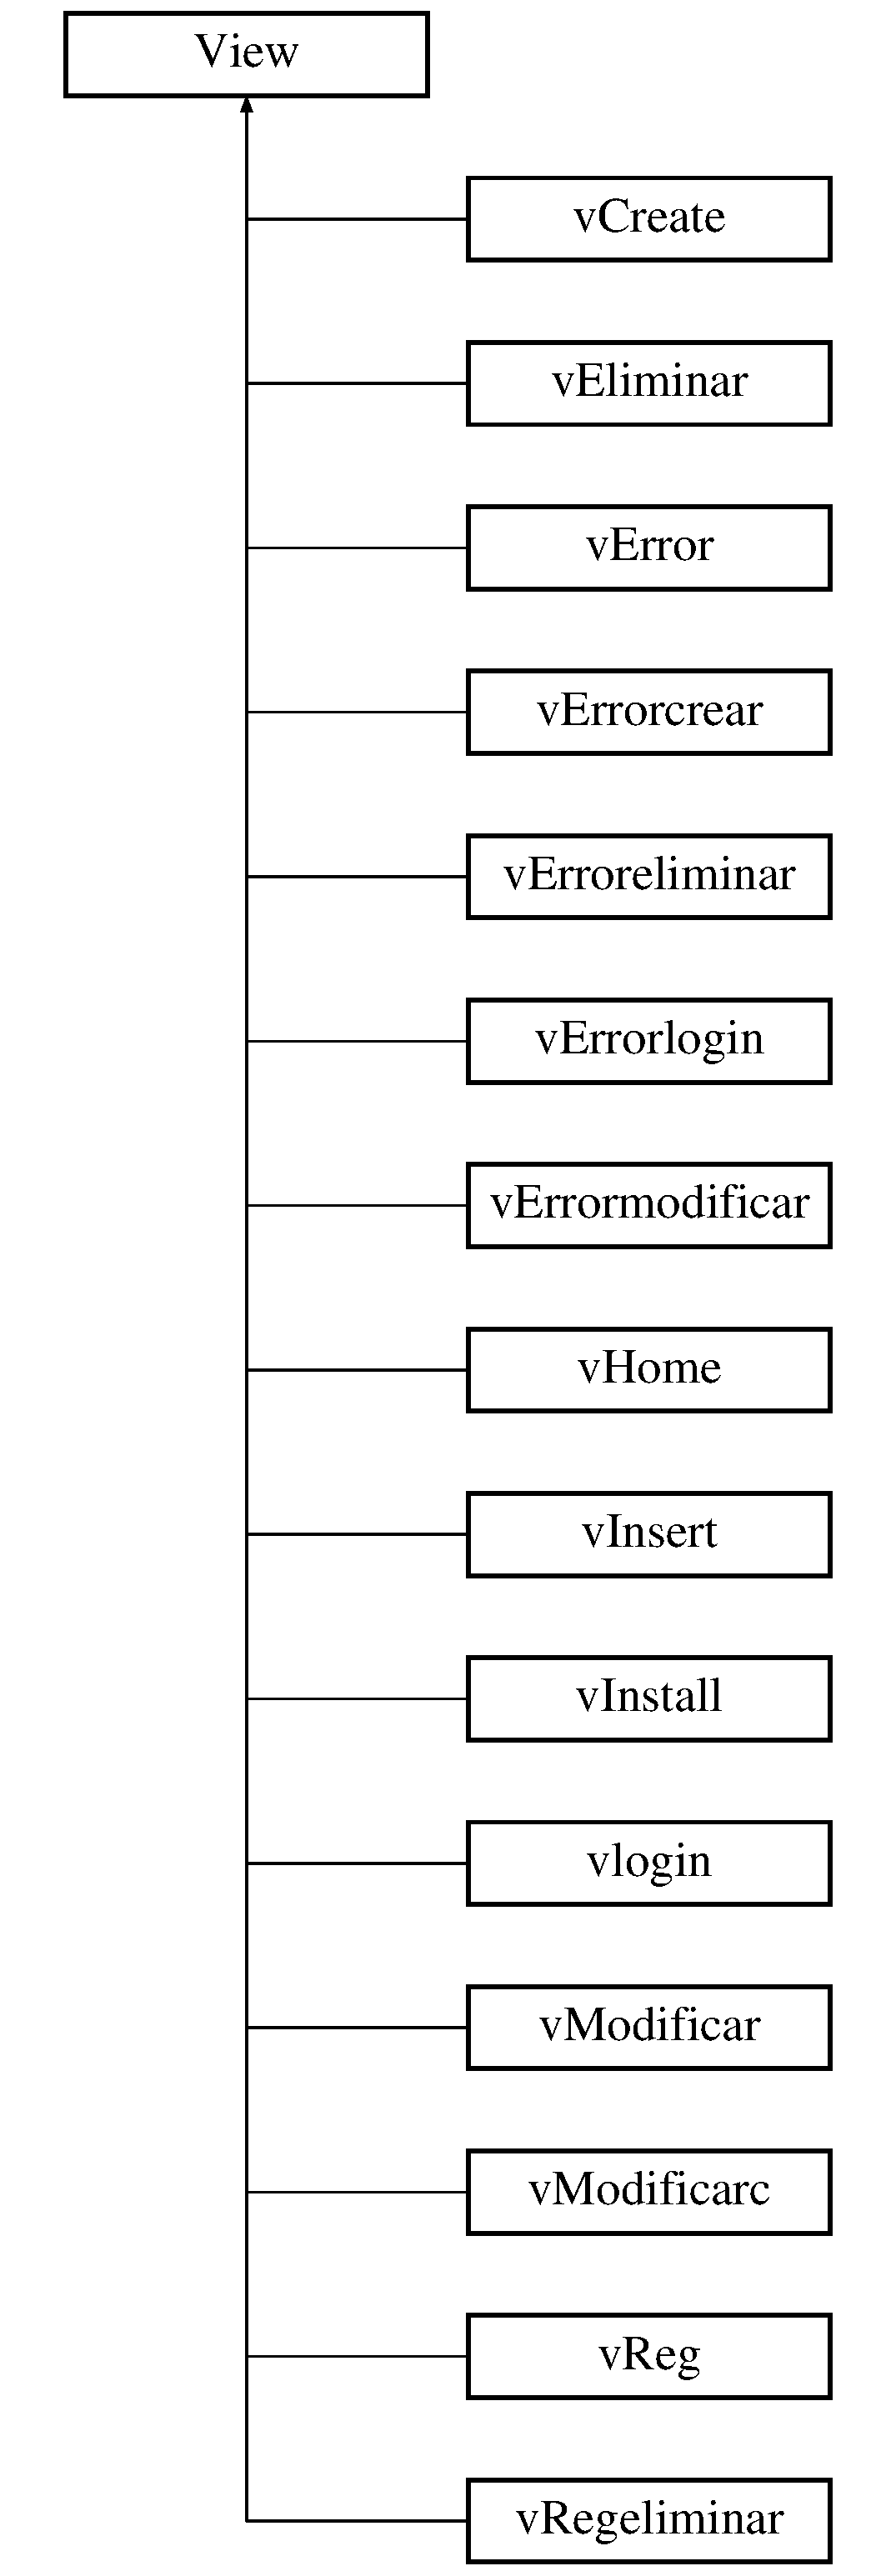
\includegraphics[height=12.000000cm]{class_view}
\end{center}
\end{figure}
\subsection*{Métodos públicos}
\begin{DoxyCompactItemize}
\item 
\hypertarget{class_view_a0566cdd65c004851d2ba7fb0b0fc19f6}{}{\bfseries \+\_\+\+\_\+construct} (\$contents)\label{class_view_a0566cdd65c004851d2ba7fb0b0fc19f6}

\end{DoxyCompactItemize}
\subsection*{Atributos protegidos}
\begin{DoxyCompactItemize}
\item 
\hypertarget{class_view_ab17fbe2ab68dbf274177a2b974b4eb23}{}{\bfseries \$reg}\label{class_view_ab17fbe2ab68dbf274177a2b974b4eb23}

\end{DoxyCompactItemize}


\subsection{Descripción detallada}
class \hyperlink{class_view}{View} access to registry and loads the corresponding template 

La documentación para esta clase fue generada a partir del siguiente fichero\+:\begin{DoxyCompactItemize}
\item 
sys/view.\+php\end{DoxyCompactItemize}

\hypertarget{classv_insert}{}\section{Referencia de la Clase v\+Insert}
\label{classv_insert}\index{v\+Insert@{v\+Insert}}
Diagrama de herencias de v\+Insert\begin{figure}[H]
\begin{center}
\leavevmode
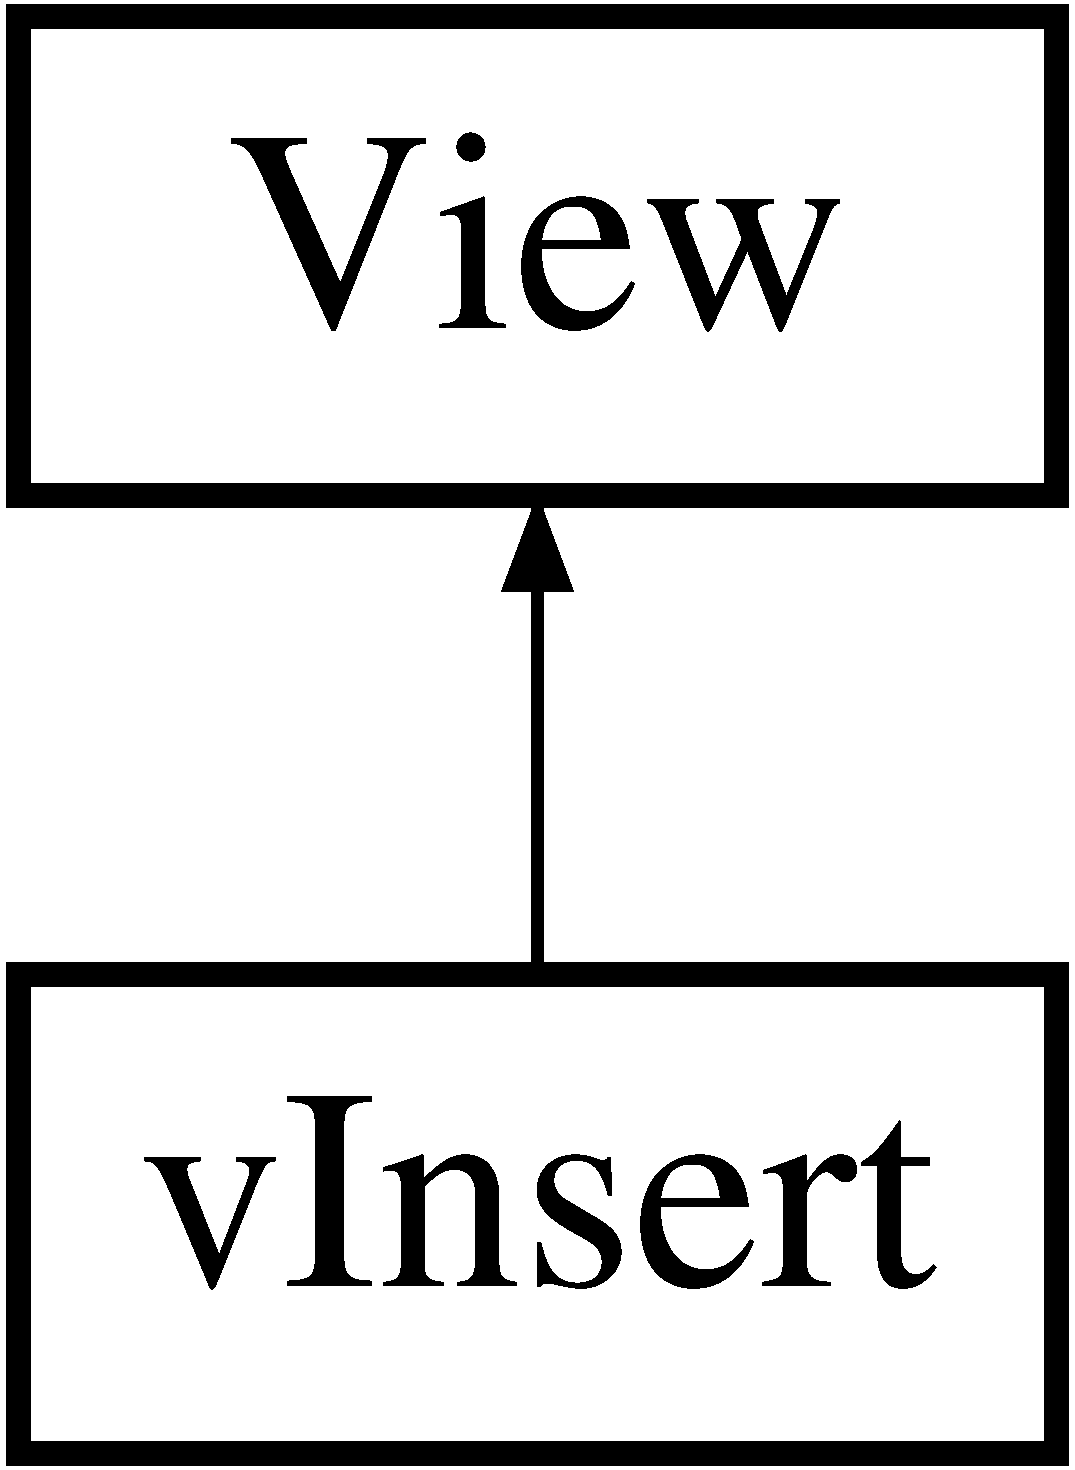
\includegraphics[height=2.000000cm]{classv_insert}
\end{center}
\end{figure}
\subsection*{Otros miembros heredados}


La documentación para esta clase fue generada a partir del siguiente fichero\+:\begin{DoxyCompactItemize}
\item 
app/views/vinsert.\+php\end{DoxyCompactItemize}

\hypertarget{classv_install}{}\section{Referencia de la Clase v\+Install}
\label{classv_install}\index{v\+Install@{v\+Install}}
Diagrama de herencias de v\+Install\begin{figure}[H]
\begin{center}
\leavevmode
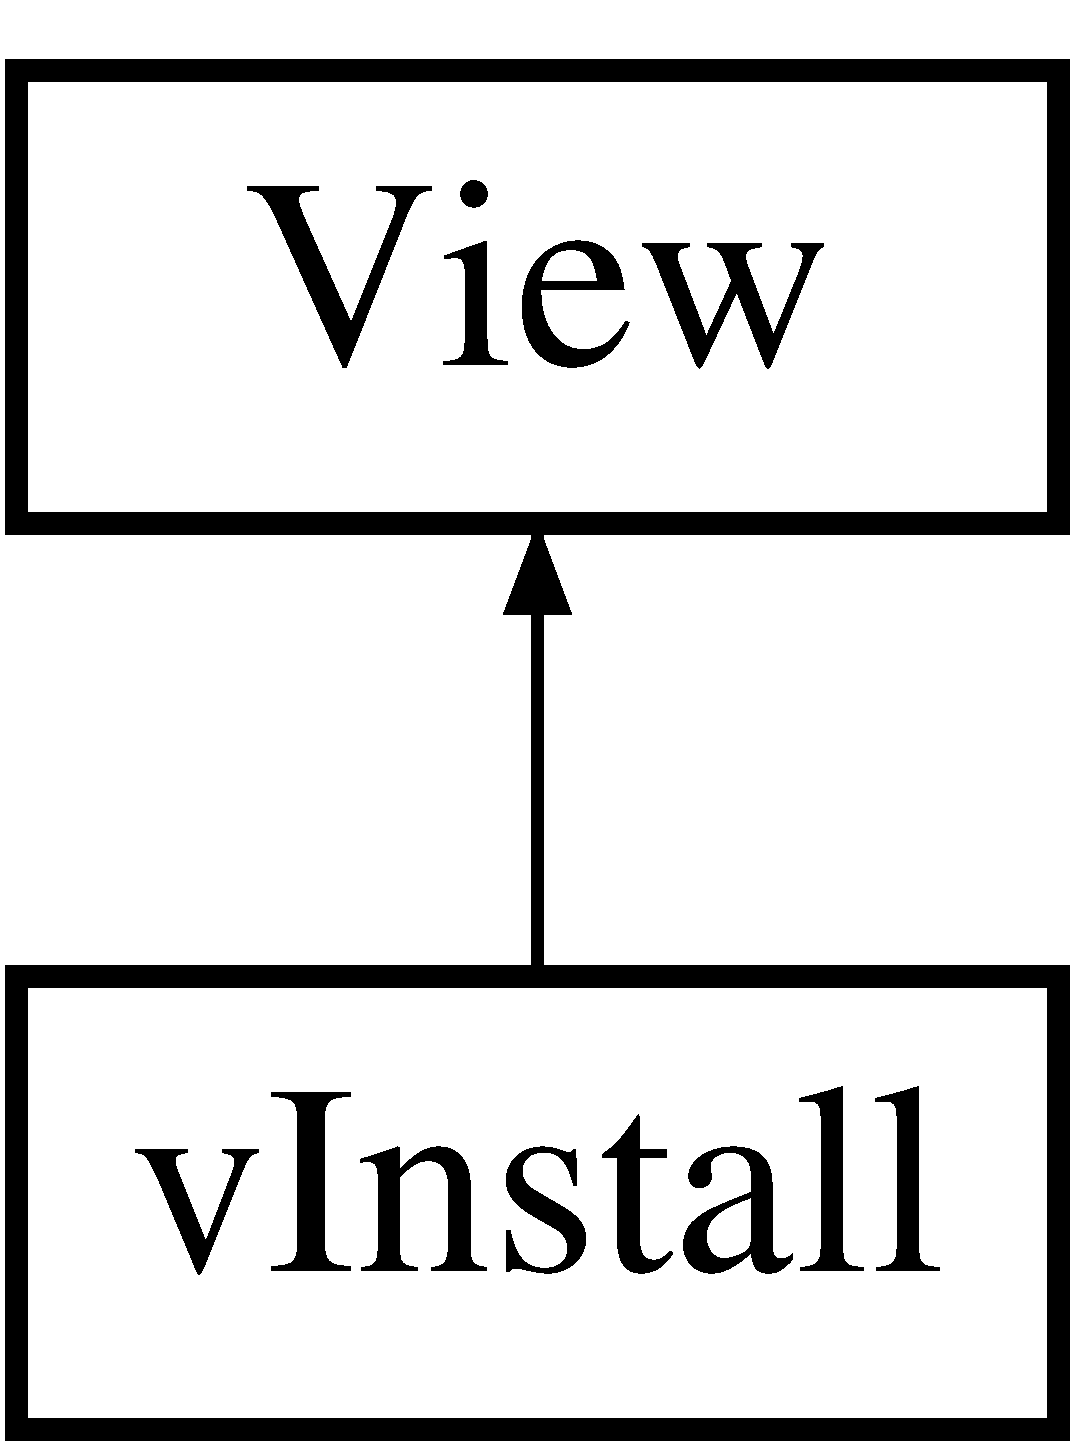
\includegraphics[height=2.000000cm]{classv_install}
\end{center}
\end{figure}
\subsection*{Otros miembros heredados}


La documentación para esta clase fue generada a partir del siguiente fichero\+:\begin{DoxyCompactItemize}
\item 
app/views/vinstall.\+php\end{DoxyCompactItemize}

\hypertarget{classvlogin}{}\section{Referencia de la Clase vlogin}
\label{classvlogin}\index{vlogin@{vlogin}}
Diagrama de herencias de vlogin\begin{figure}[H]
\begin{center}
\leavevmode
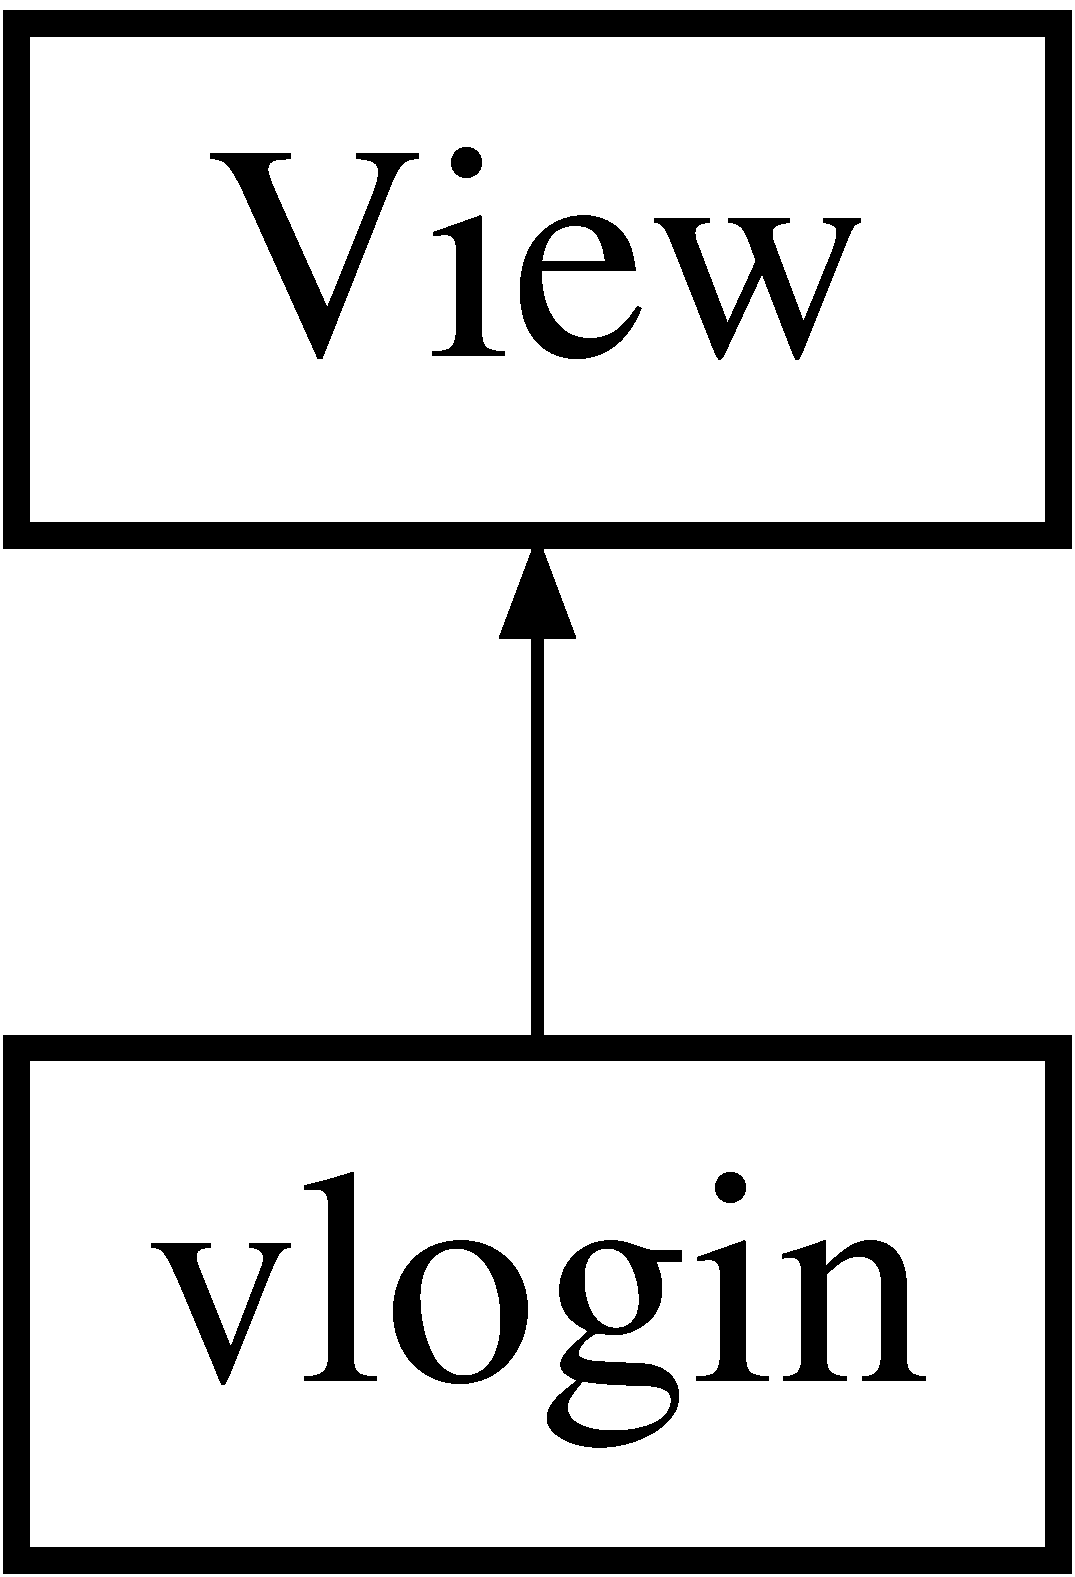
\includegraphics[height=2.000000cm]{classvlogin}
\end{center}
\end{figure}
\subsection*{Otros miembros heredados}


La documentación para esta clase fue generada a partir del siguiente fichero\+:\begin{DoxyCompactItemize}
\item 
app/views/vlogin.\+php\end{DoxyCompactItemize}

\hypertarget{classv_modificar}{}\section{Referencia de la Clase v\+Modificar}
\label{classv_modificar}\index{v\+Modificar@{v\+Modificar}}
Diagrama de herencias de v\+Modificar\begin{figure}[H]
\begin{center}
\leavevmode
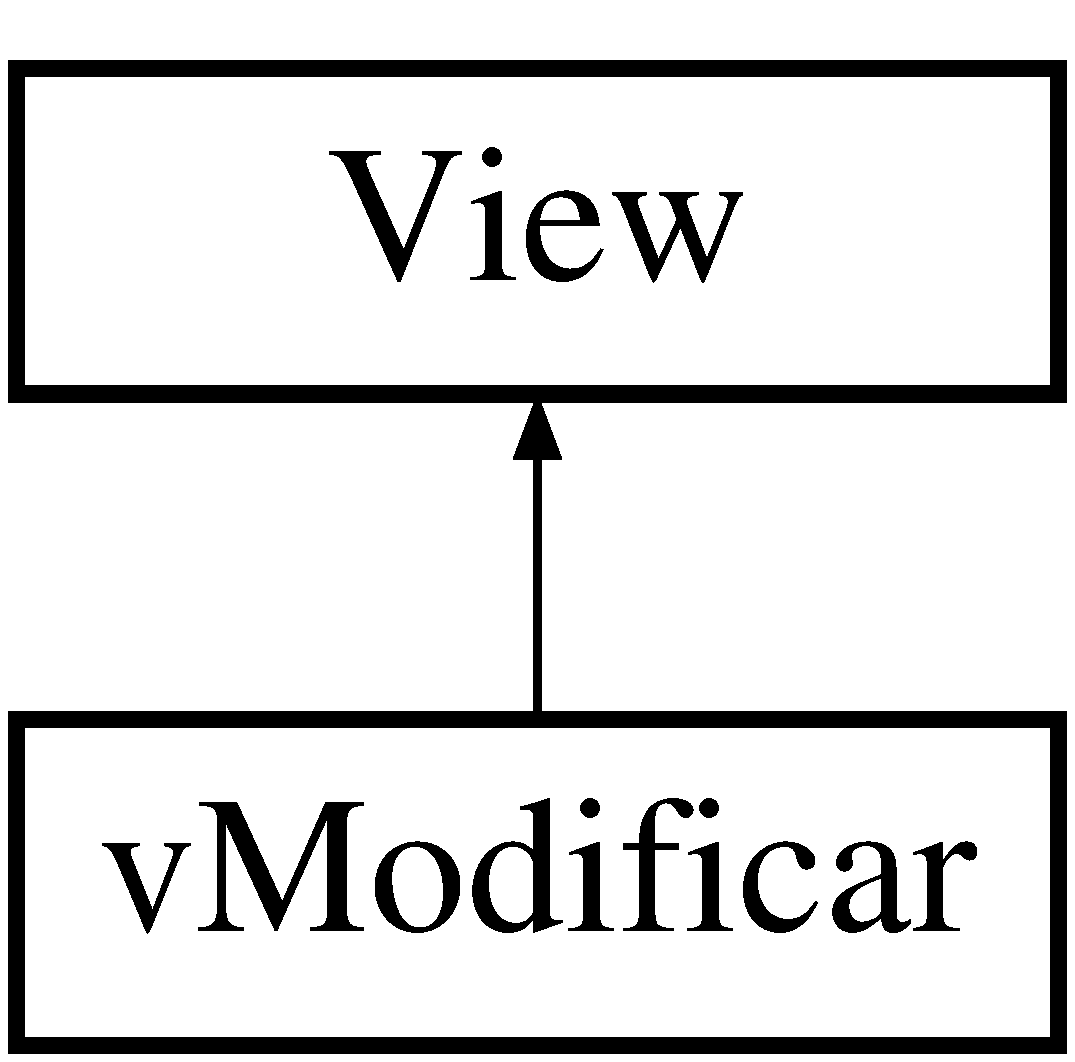
\includegraphics[height=2.000000cm]{classv_modificar}
\end{center}
\end{figure}
\subsection*{Otros miembros heredados}


La documentación para esta clase fue generada a partir del siguiente fichero\+:\begin{DoxyCompactItemize}
\item 
app/views/vmodificar.\+php\end{DoxyCompactItemize}

\hypertarget{classv_modificarc}{}\section{Referencia de la Clase v\+Modificarc}
\label{classv_modificarc}\index{v\+Modificarc@{v\+Modificarc}}
Diagrama de herencias de v\+Modificarc\begin{figure}[H]
\begin{center}
\leavevmode
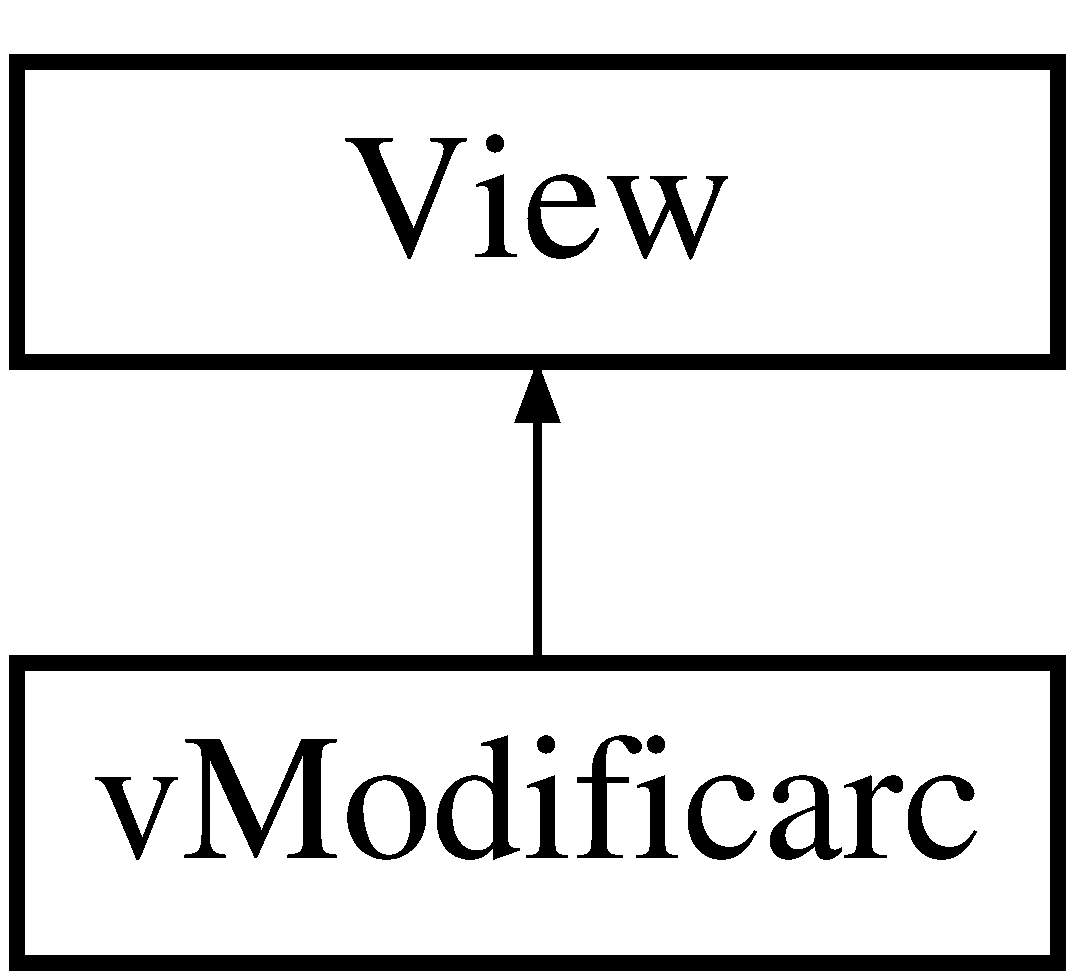
\includegraphics[height=2.000000cm]{classv_modificarc}
\end{center}
\end{figure}
\subsection*{Otros miembros heredados}


La documentación para esta clase fue generada a partir del siguiente fichero\+:\begin{DoxyCompactItemize}
\item 
app/views/vmodificarc.\+php\end{DoxyCompactItemize}

\hypertarget{classv_reg}{}\section{Referencia de la Clase v\+Reg}
\label{classv_reg}\index{v\+Reg@{v\+Reg}}
Diagrama de herencias de v\+Reg\begin{figure}[H]
\begin{center}
\leavevmode
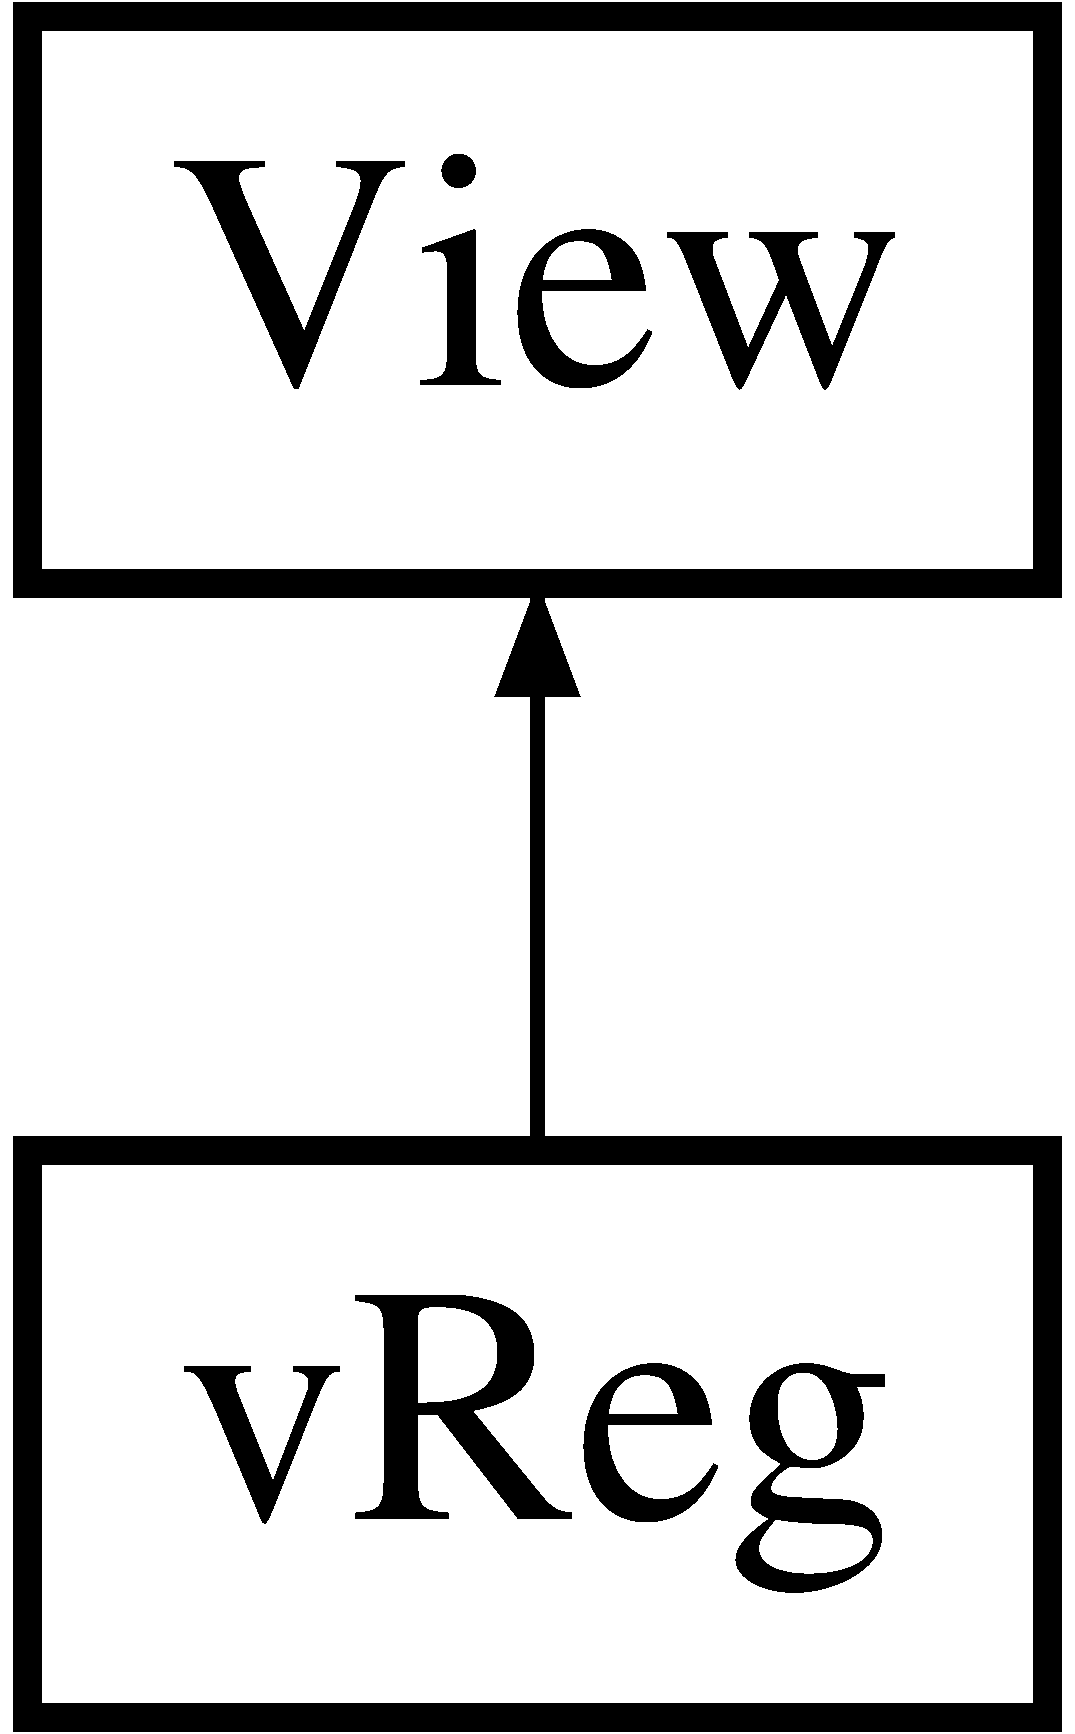
\includegraphics[height=2.000000cm]{classv_reg}
\end{center}
\end{figure}
\subsection*{Otros miembros heredados}


La documentación para esta clase fue generada a partir del siguiente fichero\+:\begin{DoxyCompactItemize}
\item 
app/views/vreg.\+php\end{DoxyCompactItemize}

\hypertarget{classv_regeliminar}{}\section{Referencia de la Clase v\+Regeliminar}
\label{classv_regeliminar}\index{v\+Regeliminar@{v\+Regeliminar}}
Diagrama de herencias de v\+Regeliminar\begin{figure}[H]
\begin{center}
\leavevmode
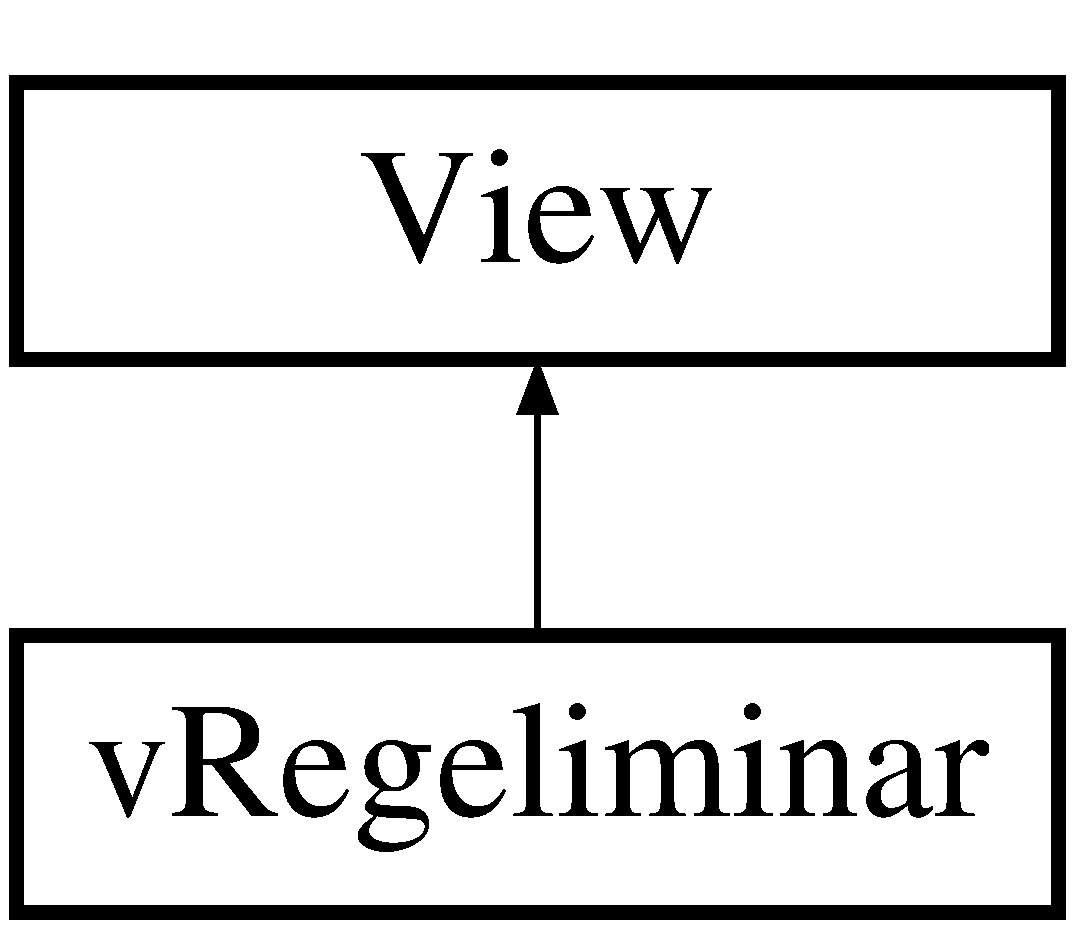
\includegraphics[height=2.000000cm]{classv_regeliminar}
\end{center}
\end{figure}
\subsection*{Otros miembros heredados}


La documentación para esta clase fue generada a partir del siguiente fichero\+:\begin{DoxyCompactItemize}
\item 
app/views/vregeliminar.\+php\end{DoxyCompactItemize}

%--- End generated contents ---

% Index
\backmatter
\newpage
\phantomsection
\clearemptydoublepage
\addcontentsline{toc}{chapter}{Índice}
\printindex

\end{document}
